\documentclass[a4paper,12pt]{book}[2004/02/16]
\usepackage{listings}
\usepackage{amsmath, amsthm}% Required
\usepackage{blindtext}
\usepackage{wrapfig}
\usepackage{amssymb}% Used for 3 symbols, lines below ensure file
% will compile without it.
\usepackage{tcolorbox}
\providecommand{\leqq}{\leq}
\providecommand{\geqq}{\geq}
\providecommand{\therefore}{\mathrel{{.}\kern-.05em\raise.40em\hbox{.}\kern-.05em{.}}}
\usepackage{mhchem}
\usepackage{stmaryrd}
\usepackage[export]{adjustbox}
\usepackage{a4wide}% Optional; chooses nicer margins for a4 paper
\usepackage{tcolorbox}
\usepackage{stmaryrd}% Used for \olessthan. 
\usepackage{fontspec}
\usepackage{parskip}
% Could substitute {txfonts/pxfonts} package and use \circledless.
% Line below ensures file will compile without it.
\providecommand{\olessthan}{(<)}

\usepackage{epic,eepicemu}% Required for figs 4, 5, 7, 12, 14, 16, 17, 18, 20
% If compiling via latex+dvips, put eepic in place of eepicemu.
\usepackage{graphics}
\usepackage{graphicx}

\usepackage{longtable}% Required for Wiley catalogue at back.
% If unavailable, remove this, or split into a number of shorter tables
% that fit on one page.

\usepackage{color}% If unavailable, the file will compile if the 2nd
% newcommand below is uncommented and the one above it commmented out.
% Textual corrections will be underlined instead of highlighted in grey.
\providecommand{\definecolor}[3]{}
\providecommand{\colorbox}[2]{#2}
\setlength{\fboxsep}{1pt}
\definecolor{corr}{rgb}{0.89,0.89,0.89}
\newcommand{\correction}[2]{\colorbox{corr}{#1}}
%\newcommand{\correction}[1]{\underline{#1}}

\usepackage[pdftex]{graphicx}% If unavailable, use "graphics" in place of
% "graphicx".  If both are unavailable or if pictures are absent,
% add the option "draft" into the documentclass.  Figures will not appear,
% but nor will hyperlin ks.  Or, don't use draft mode but manually remove all
% the figures; hyperlinks will still work.
% If compiling via dvips, change [pdftex] to [dvips] and convert images to
% Encapsulated Post Script.
\usepackage{makeidx}% If unavailable, the following line makes the file
% compile.  Do not run makeindex.  Document will have no index.
\providecommand{\printindex}{}

\usepackage[pdftex,plainpages=false,pdfpagelabels,colorlinks,linkcolor=blue]{hyperref}
% If unavailable, the following lines ensure the file compiles, but
% the document will not have hyperlinks.
\providecommand{\hyperlink}[2]{#2}
\providecommand{\hypertarget}[2]{#2}
\providecommand{\phantomsection}{}
\providecommand{\pdfbookmark}[3][0]{}
\providecommand{\hypersetup}[1]{}

%%%%%%%%%%%%%%%%%%%%%%%%%%%%% PREAMBLE %%%%%%%%%%%%%%%%%%%%%%%%%%%%%%%

%%%%%%%% Fix hyperref page links
\makeatletter
\AtBeginDocument{\def\pageref#1{%
  \expandafter\@pagesetref\csname r@#1\endcsname\@empty{#1}}}
\makeatother
%%%%%%%% Hyperref setup
\hypersetup{
pdfauthor = {Aitzaz Imtiaz},
pdftitle = {Research of The Century}
}

%%%%%%%% Special notation for intervals
\newlength{\intwidth}
\newcommand{\interval}[2]{\settowidth{\intwidth}{$#1\ #2$}\overset{|\!\rule[0.25ex]{\intwidth}{0.5pt}\!|}{#1\ #2}}
\newcommand{\linterval}[2]{\settowidth{\intwidth}{$#1\ #2$}\overset{|\!\rule[0.5ex]{\intwidth}{0.5pt}}{#1\ #2}}
\newcommand{\rinterval}[2]{\settowidth{\intwidth}{$#1\ #2$}\overset{\rule[0.5ex]{\intwidth}{0.5pt}\!|}{#1\ #2}}
% For more modern notation (as at 2006) remove the above four lines
% and uncomment the following three:
%\newcommand{\interval}[2]{[#1,#2]}
%\newcommand{\linterval}[2]{[#1,#2)}
%\newcommand{\rinterval}[2]{(#1,#2]}

%%%%%%%% Special inequality signs
\newlength{\chevron}
\settowidth{\chevron}{$<$}
\newlength{\equals}
\settowidth{\equals}{$=$}
\addtolength{\chevron}{\equals} % to get < and = centred wrt each other
\newcommand{\weirdineq}[1]{%
        \mathbin{\lower0.3ex\hbox{$#1$\kern-.5\chevron\raise1.25ex\hbox{$=$}}}
}
\newcommand{\qqle}{\weirdineq{<}}
\newcommand{\qqge}{\weirdineq{>}}

%%%%%%%% Sections formatting
\renewcommand{\thesection}{\S~\arabic{section}}
\renewcommand{\sectionmark}[1]{}
\renewcommand{\chaptermark}[1]{\markboth{THE PHILOSOPHY}{#1}}

%%%%%%%% Theorems formatting (book also used parindent but it's ugly!)
\newtheoremstyle{itheorem}{}{}{\itshape}{}{\bfseries}{.}{ }{#1\if!#3!\else\ \fi\thmnote{#3}}
\newtheoremstyle{icorollary}{}{}{}{}{\itshape}{.---}{0pt}{#1}
\newtheoremstyle{numcorollary}{}{}{}{}{\itshape}{.}{ }{#1\if!#3!\else\ \fi\thmnote{#3}}
\newtheoremstyle{idefinition}{}{}{}{}{\bfseries}{.---}{0pt}{}
\newtheoremstyle{ilemma}{}{}{\itshape}{}{\bfseries}{.---}{0pt}{#1\if!#3!\else\ \fi\thmnote{#3}}
\newtheoremstyle{iother}{}{}{\itshape}{}{\bfseries}{.---}{0pt}{\thmnote{#3}}
\theoremstyle{ilemma}
\newtheorem*{lemma}{Lemma}
\theoremstyle{itheorem}
\newtheorem{theorem}{Theorem}
\theoremstyle{iother}
\newtheorem{other}{}
\theoremstyle{icorollary}
\newtheorem{corollary}{Corollary}
\theoremstyle{numcorollary}
\newtheorem{ncorollary}{Corollary}
\theoremstyle{idefinition}
\newtheorem*{definition}{Definition}
\newtheorem*{definitions}{Definitions}
\newtheorem*{defnorder}{Definition of Order}


\renewcommand{\proofname}{\upshape\bfseries Proof}
\renewcommand{\qedsymbol}{}
%%%%%%%% Miscellaneous
\renewcommand{\dfrac}[2]{\frac{#1}{#2}}% Book always used displaystyle
% for fractions, but it makes text ugly!
\renewcommand{\indexname}{\protect\label{index}\protect\pdfbookmark[0]{INDEX.}{index}\protect\plainindexname{}INDEX.}
\newcommand{\plainindexname}{\gdef\indexname{INDEX.}}


\makeindex
\begin{document}
\normalsize
\frontmatter
\title{\label{titlepage}\pdfbookmark[0]{Title Page.}{titlepage}%
THE ESSAYS \\
{\small ON}\\
{\Huge SCIENTIFIC PHILOSOPHY\\[1ex]}
{\Large A BOOK ANALYZING THE GOOD AND EVIL}
}

\author{{\small BY}\\
Aitzaz Imtiaz\\
\textit{Beaconhouse School System, Senior Boys Branch BSTRB}\\
}
\date{%
\textit{FIRST EDITION}\\
{\small BELGIUM EXCLUSIVE}\\
\vspace{0.2\textheight}
RAWALPINDI\\
NEUROSTOL PAKISTAN \& AMAZON INTERNATIONAL\\
\textsc{FRANCE: NEUROSTOL FRANCE \& AMAZON FRANCE}\\
2022
}
\maketitle
%-----File: 006.png---Folio ii-------
\begin{center}
\vspace*{0.4\textheight}
Copyright, 2022\\
\textsc{by\\
Aitzaz Imtiaz\\}
\vfill
PRESENTED TO YOU BY NEUROSTOL PUBLISHING
\end{center}
\newpage
%-----File: 007.png---Folio iii------
\newpage
\begin{center}

In a reserved Dedication to:\\
\Huge
Ma'am Almas Wajid\\
\bigskip
\normalsize
for generally encouraging me to write this book, exploring Science and God as a philosopher is one of my greatest achievements now! \\
\bigskip
\bigskip
\bigskip
Never going to forget that one person, the one who helped me a lot with my emotional well-being, when the world closed its doors on me, and that person helped me with struggling endeavors, the heartiest dedication to,\\
\Huge
Yasmine Pijck\\
\bigskip
\normalsize
The time spent talking from two distant points from the planet is still memorable for me.\\
\end{center}
\newpage
\Huge
\begin{center}
Honorable Mentions  
\end{center}
\normalsize
Since it is one of the best books I am on record claiming to publish, I wish to give honorable mentions to people who actually made me happy and helped me with my old war with depression and hallucinations.
\newline
\newline
BE Yasmine Pijck  (linked to: Imtiaz Pijck Cubic Solution)
\newline
UA Dmytro Kolibabchuk (linked to: Katsman Table)
\newline
PK Maryam Taufiq
\newline
UK Sophie Fraser
\newline
UA Petro Olievsky (linked to: Olievsky Table)
\newline
UA Lavra Olievsky (linked to: Olievsky Table)
\newline
FR $\dagger$Sophie Germain (linked to: Imtiaz Germain Primes)
\newline
PK Sir Muhammad Ali
\newline
PK Sir Abid Hussain
\newline
PK Saad Muneer
\newline
PK Saad Nawaz
\newline
PK Ali Wajid (linked to: Imtiaz Wajid Genotype Formula)
\newline
PK Subhan Rafiq
\newline
PK Ahmed Sultan
\newline
PK Muhammad Dawood
\newline
PL Joanna Asia

\chapter*{ABSTRACT}
The following book was written, in the analysis of modern Physics, Mathematics and Sciences. With an artistic approach, carefully I assembled my thoughts on the philosophical nature of happenings around me. The following book was carefully written keeping in mind not only the opinions but on fact-based evaluations of modern philosophical improvements.

\bigskip
[signed]


\includegraphics[]{signature.png}

All yours!
% Generator pre-programmed
\chapter*{THE IWG FORMULA}
The Imtiaz-Wajid Genotype Formula has been written down in this book (does not links to though) and has been mentioned as my first research on Biology which keeps the record of my fastest research by time. The AG series took four years to make, Javed Effect took three months, Theory of Centrifugal Forces on Black Holes took a week, while the formation of IWG just took five minutes of a lecture I just breached!

Geneticists generally have an interest in Breeding experiments and use the idea of Test Cross. As we know the dominant homozygous group and the recessive homozygous group, the idea of Test Cross in the modeling seems like a failure. Basically, the test cross may be a lengthy process, and to shorten it, we might create some models\footnote{The one in O Levels Singapore Biology groups are far more crazy. Perhaps usually teachers show a combination table which can be considered such a process.}.

On a usually normal Thursday, when studying Galois Theory, I saw Ma'am Almas teaching the concept of Genotypes to one of her students\footnote{I actually do not know Biology really well seriously}. Here is what I noted from that lecture outside the bench going on:

    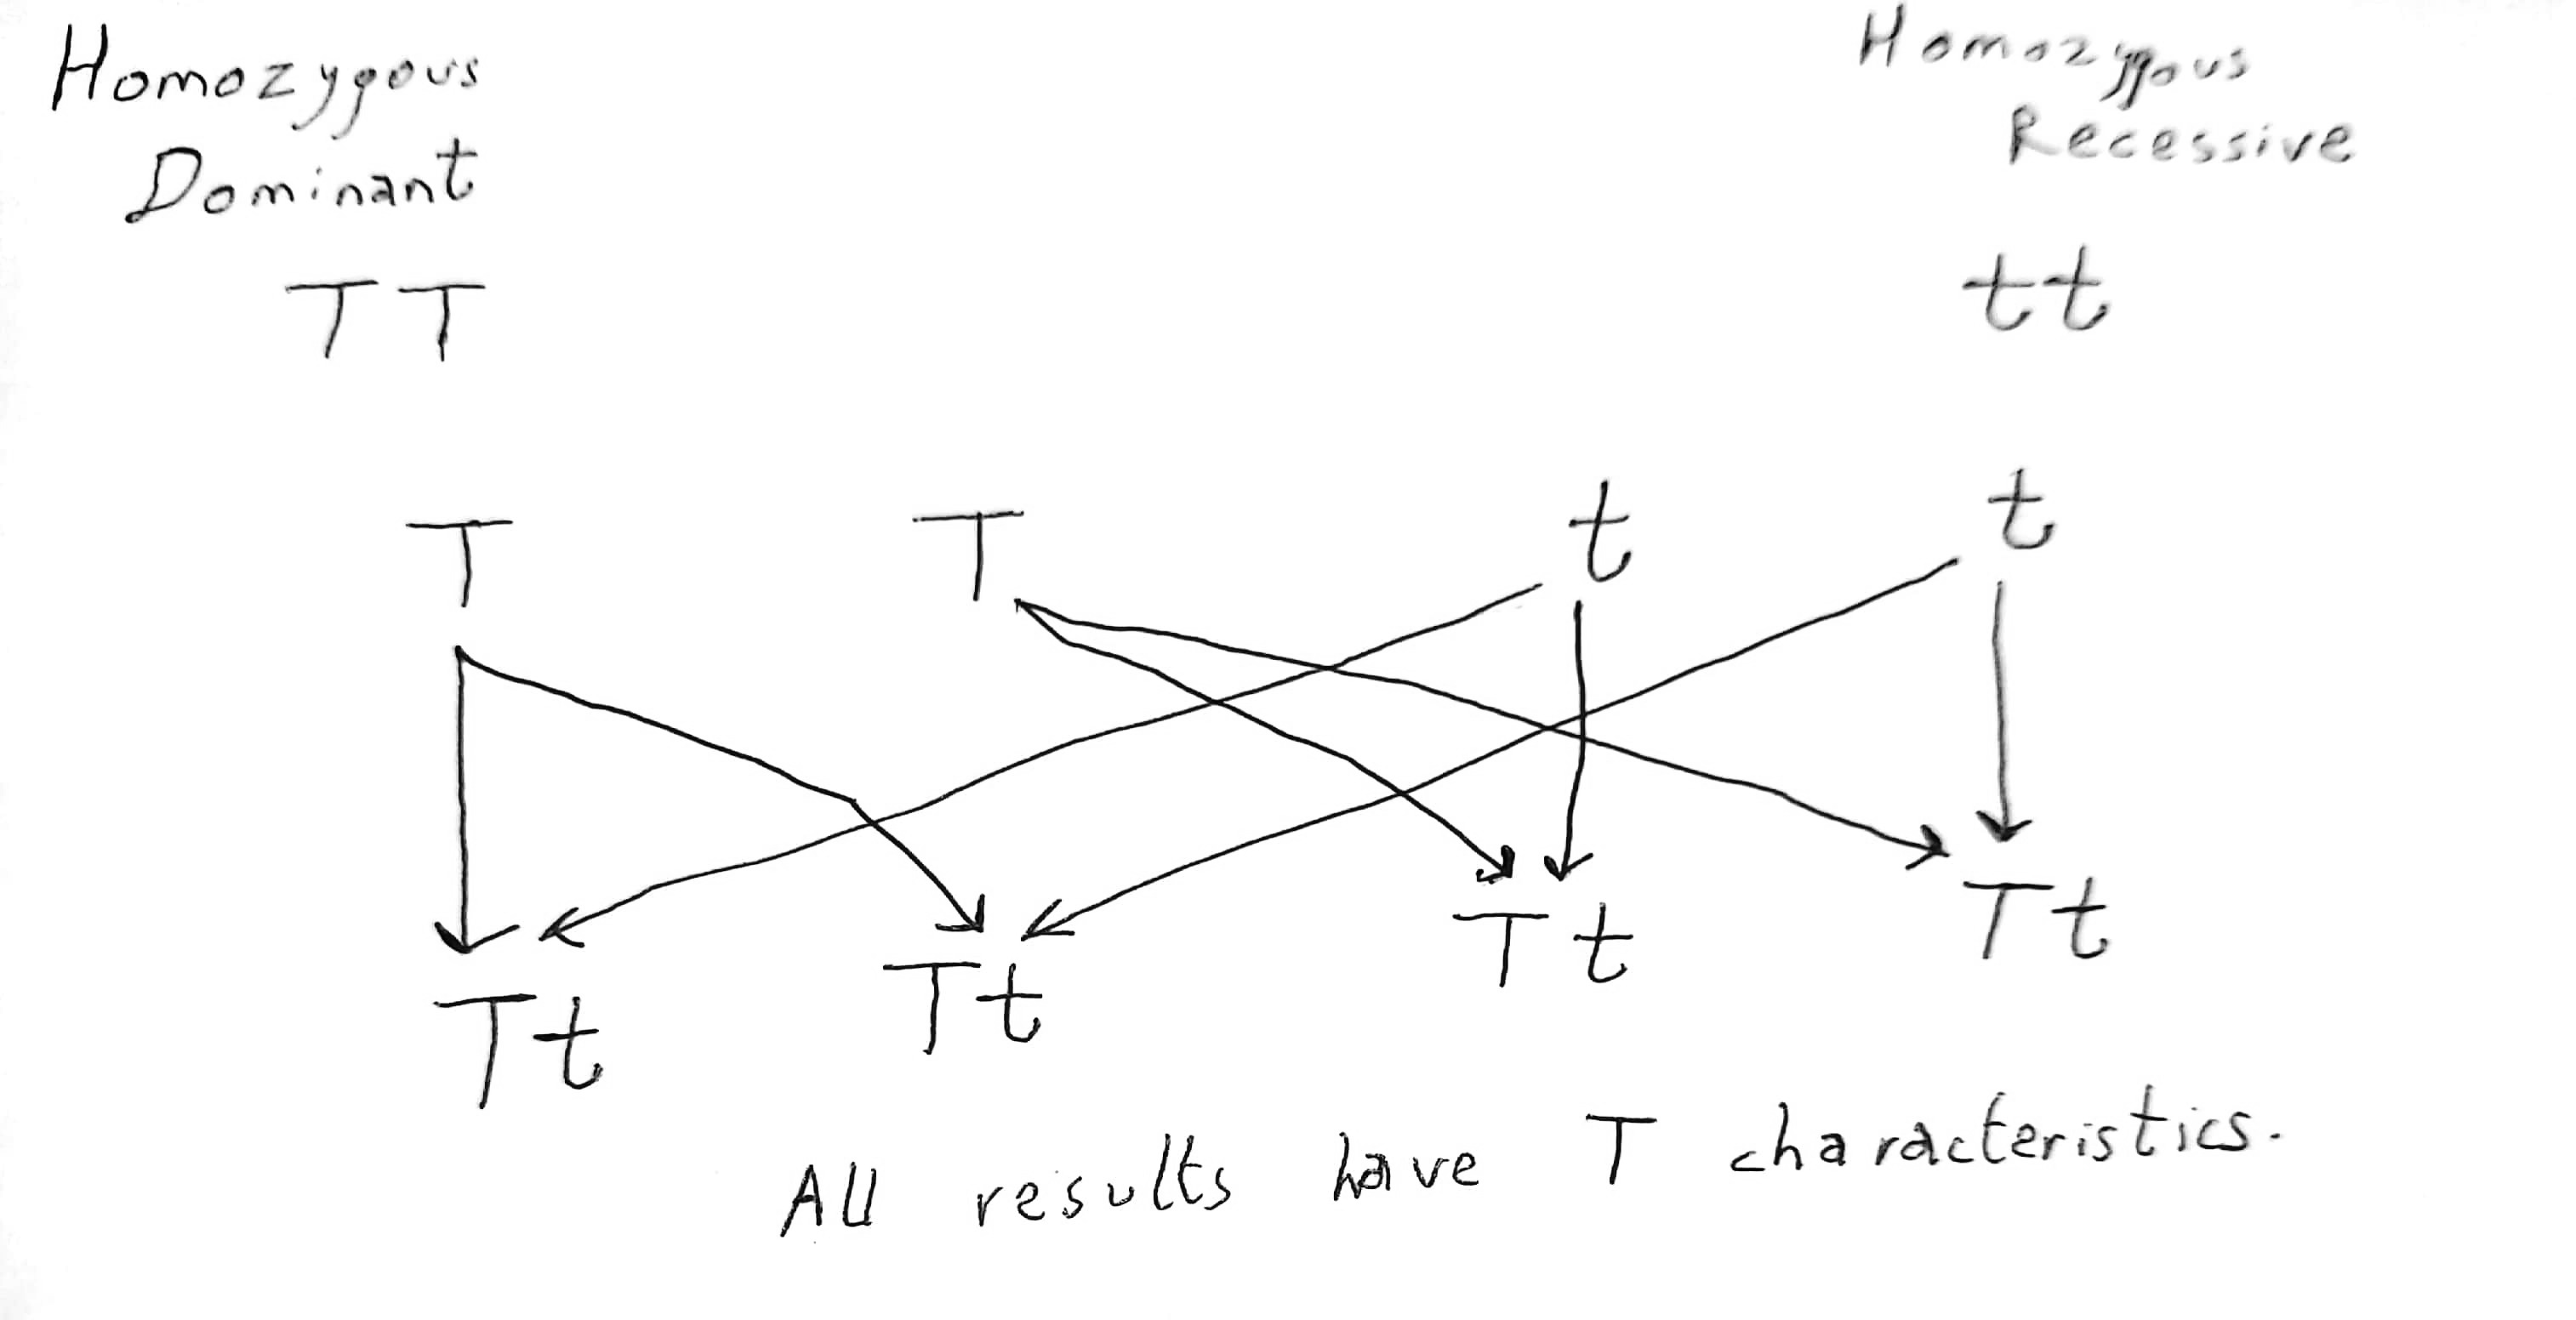
\includegraphics[width=\textwidth,height=80mm]{New Doc 12-12-2022 19.57_3-modified.jpg}

Apart from my weird handwriting, we can note that the partition occurs at an initial stage such that:
$$
f(n) = 1+1+1...:1+1+1...=n
$$
Here $n$ is the count of elements of the organisms. In our case, the result of possible results of Combinations would be:
$$
{}^{4}C_{2}-2 = \frac{4!}{2!(4-2)!}-2
$$
$$
= \frac{3!}{1}-2
$$
$$
=6-2=4
$$
We will now define a Biological function now:
$$
{}^{2}G_{2}
$$
Now ${}^{2}G_{2}$ will return the information of the result of total offspring probabilities we will get here as a result of the Test Cross.
$$
{}^{2}G_{2} = {}^{4}C_{2}-2
$$
The result we have seen lands out the total numbers of genotypes.  We can see ${}^{n}G_{r}$ as $n$ is the total parental genotypes count, and $r$ as the total elements inside the structure. The formula for such can be represented by:
$$
{}^{n}G_{r} = {}^{2n}C_{r} -  n(r-1)
$$
The following formula \footnote{The following formula is discovered by me, there is less probability it was discovered before}  helps solve as a Zenotype Offspring count. Now, let us go for something which is a bit scarier.

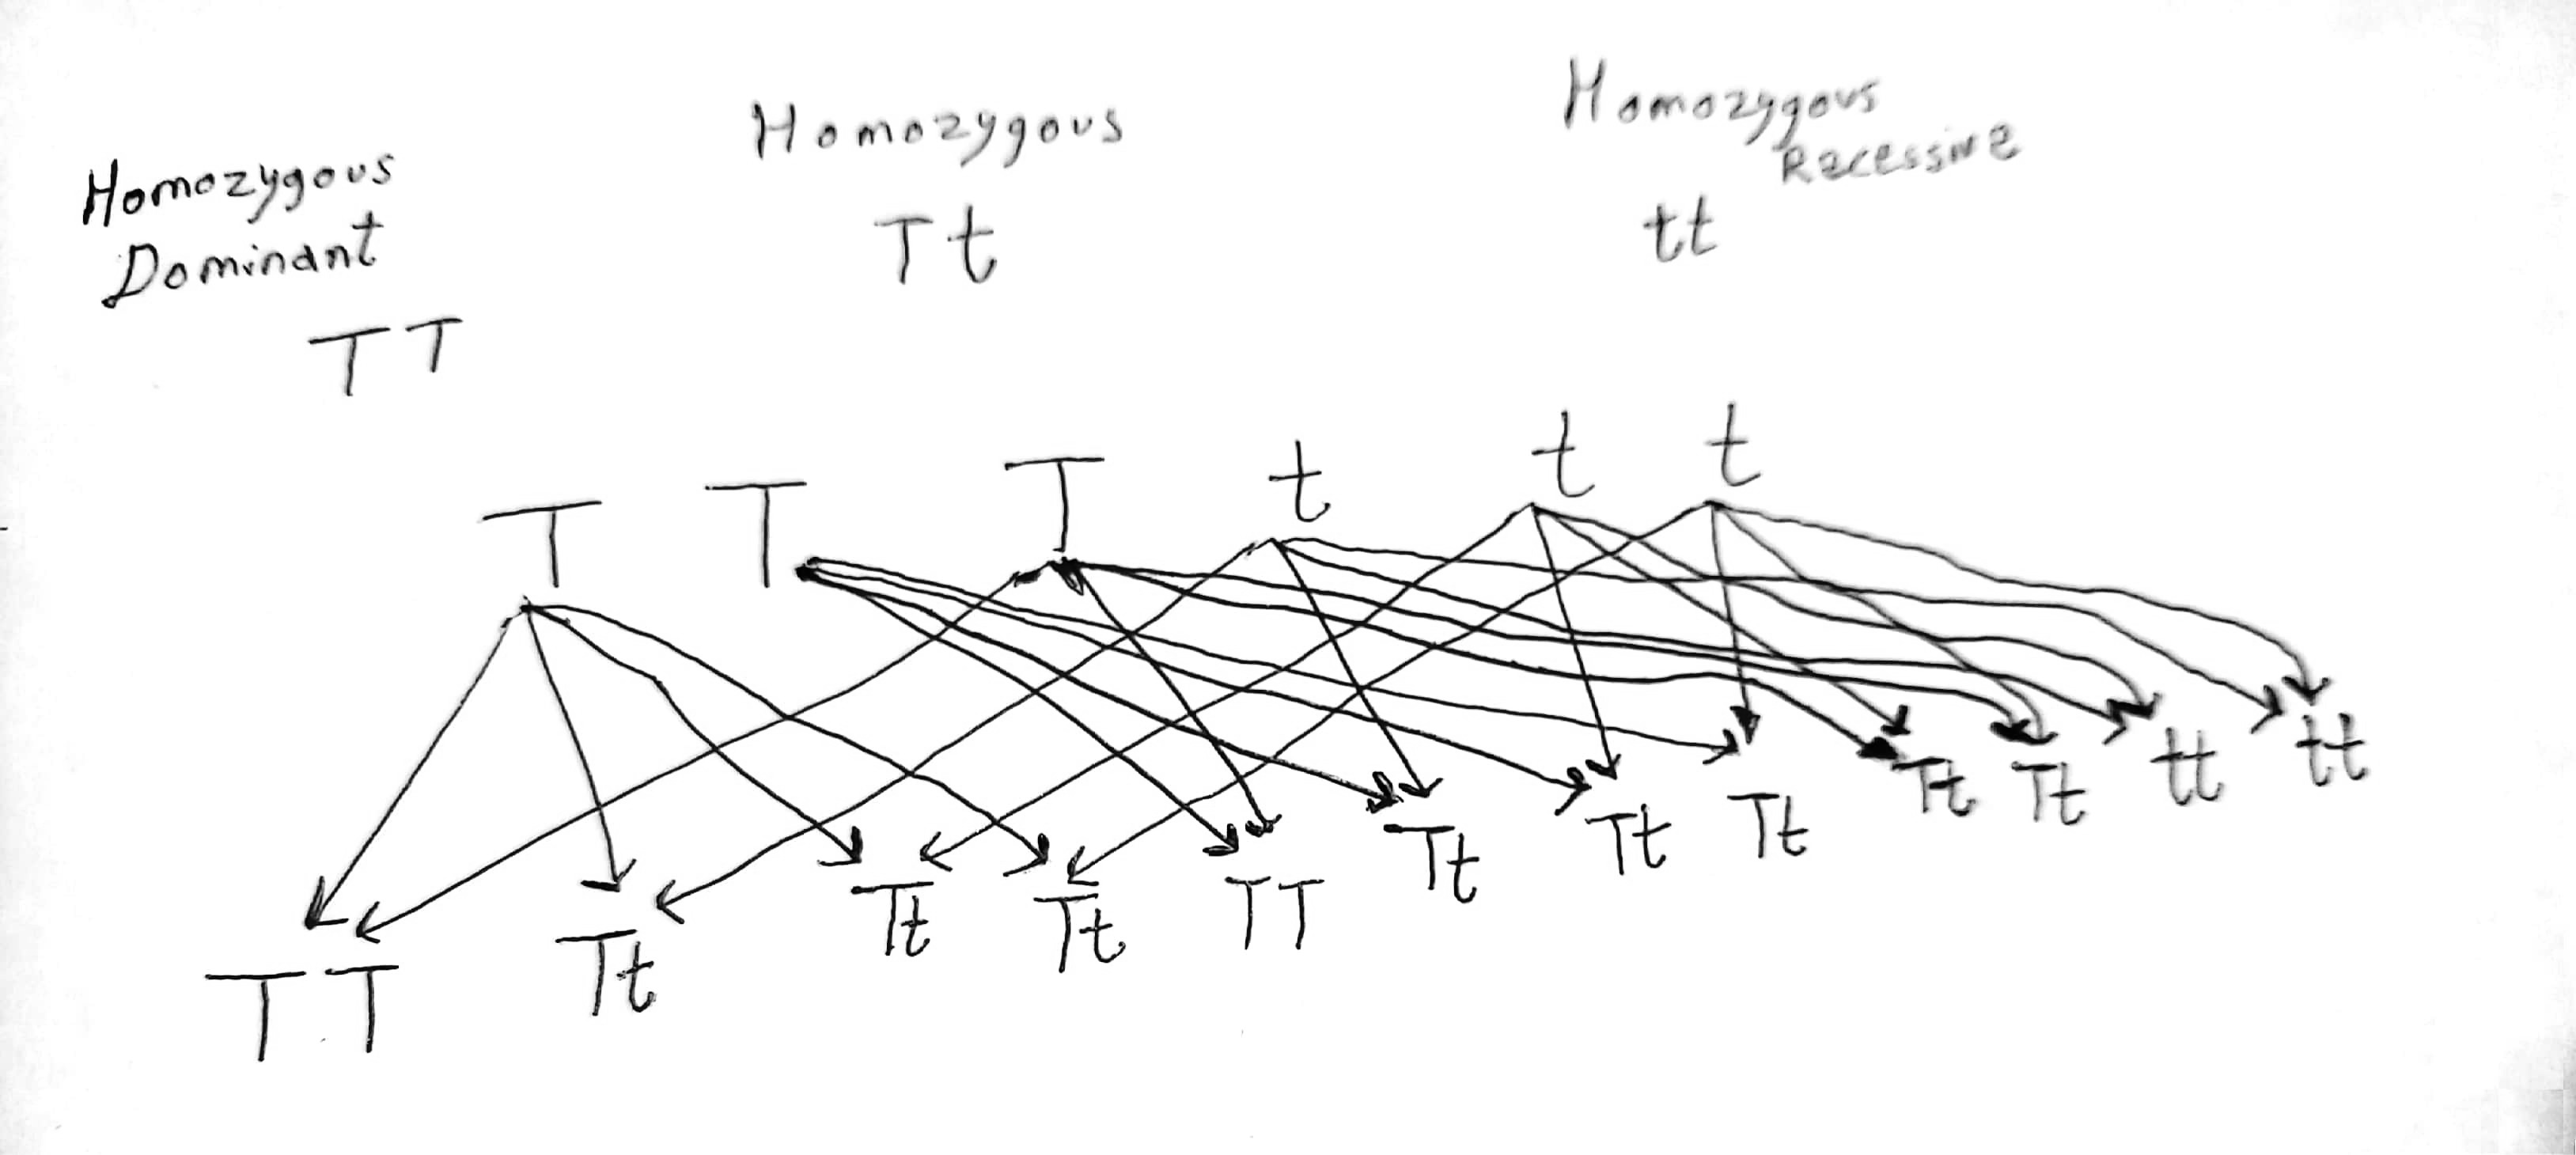
\includegraphics[width=\textwidth]{New Doc 12-12-2022 19.57_4-modified.jpg}

We will use the formula of ${}^{n}G_{r}$ first to check whether our value returned is 12 or not.
$$
{}^{3}G_{2} = {}^{6}C_{2} -  3(2-1)
$$
$$
=\frac{6!}{2!(4!)} - 3
$$
$$
=\frac{30}{2!} - 3
$$
$$
=15-3
$$
$$
=12
$$
\chapter*{THE IMTIAZ PIJCK CUBIC SOLUTION}
If I was ever asked to explain the structure which of my research would be closest to my heart; my affirmed reply would be the Imtiaz Pijck Cubic Solution. Here is a list of what I concluded as such:
\begin{itemize}
    \item Imtiaz Pijck Cubic Solution
    \item AB Series (previously named AG Series)
    \item Imtiaz Wajid Genotype Function
    \item Contributory Effect (previously named Javed Effect)
    \item Imtiaz Germain Primes
    \item Theory of Liquefied Beginning 
\end{itemize}
We know that a cubic equation $f(x)=ax^3+bx^2+cx+d$ can be solved, though with difficult ways and the Cardano formula. Usually, students like me use the Hit and Trial method, but there are some secret ways to find the cubic solution if they have root 1. Provided that $f(1)=0$, we will give the formula that always works to find out the other roots.
$$
ax^2+bx+c=ax+b+cx^{-1}
$$
$$
ax^3+bx^2+cx=ax^2+bx+c
$$
$$
ax^3+bx^2-ax^2+cx-bx-c=0
$$
$$
ax^3+(b-a)x^2+(c-b)x-c=0
$$
Now, with this, the above result will lead one confirmed root of $x=1$. Now, we demonstrate an example of cubic equation $x^3-6x^2+11x-6=0$ and solve it. Being assured, applying 1, we get the answer as zero. We now bring it to form above,
$$
x^3+(-5-1)x^2+(6+5)x-6=0
$$
Our quadratic equation where the constants are extracted definitely includes first and last constants, 1 and c (not -c), which is 6. Our b according to the above formula is -5. Using this, we come to solve $x^2-5x+6=0$ and their roots will be the answer for the cubic formula. From here, we can declare b as a Pijck variable, a connectivity between two functions, that make two unfamiliar functions match with at least one common root shared and that the variable plays the rule in connection. Here, b is a Pijck variable binding a Quadratic function to Cubic one.
\tableofcontents
\mainmatter
\chapter{Study of Mathematics}\hypertarget{chapI}{}%[I]
\index{Number}
It is essential to ask the question, "What is its purpose and ideal?" from time to time about every human activity. What contribution does it make to the beauty of human existence? As regards those pursuits which contribute just from a distance,
by giving the instrument of life, it is well to be reminded that not
the simple reality of living is to be wanted, yet the craft of living in the
thought of incredible things. In addition, it is essential to maintain a clear prefiguring vision of the temple in which creative imagination is to be embodied in relation to vocations that have no external purpose and must be justified, if at all, as contributing to the total of the world's permanent possessions.

When it comes to the research that forms the foundation for the curriculum that the custom has chosen to instruct young minds on, the fulfillment of this requirement is, unfortunately, extremely remote—so remote that it renders the mere assertion of such a claim absurd. Great men convince humanity to pass on the mechanical knowledge necessary to cross the threshold to subsequent generations because they are fully aware of the beauty of the contemplations to which they dedicate their lives and wish that others may share in their joy. Dry know-it-alls have themselves of
the honor of imparting this information: They do not realize that it serves as a key to unlock the temple's doors; Even though they spend their entire lives on the steps leading to those holy doors, they turn their backs on the temple so firmly that it loses its very existence, and the eager youth who would like to be led into its domes and arches is told to turn around and count the steps.

Math, maybe more even than the investigation of Greece and Rome, has
experienced this blankness of its expected spot in civilization. Despite the fact that most educated men are expected to be familiar with at least some of the material, the reasons behind the custom's origin are lost in a sea of trivialities and petty nonsense. When people inquire about the purpose of mathematics, the typical response is that it makes it easier to create machines, travel between locations, and defeat foreign nations in war or commerce. The response, it is true, will probably be that mathematics trains the reasoning faculties if it is argued that these ends, all of which are of doubtful value, are not furthered by the merely elementary study required of those who do not become expert mathematicians. However, the men who provide this response are, for the most part, unwilling to abandon the teaching of certainly known fallacies, which every intelligent learner instinctively rejects. Those who advocate for its development also tend to view the reasoning ability as merely a tool for avoiding pitfalls and assisting in the discovery of guidelines for everyday life. All of these are unquestionably significant contributions to mathematics; However, none of these merit the inclusion of mathematics in every liberal education. We know that Plato thought that thinking about mathematical truths was worthy of the Deity; and Plato realized, perhaps more than any other individual, what aspects of human life are worthy of heaven. "Something that is necessary and cannot be set aside... and, if I am not mistaken, of divine necessity," he asserts, exists in mathematics. Because of the absurd application of the words to the human needs about which many speak in this context, nothing could be further from the truth.
According to Plato's assessment of mathematics, "those things without some use or knowledge of which a man cannot become a God to the world, nor a spirit, nor yet a hero, nor able earnestly to think and care for man" (Laws, page 818)\footnote{Proffessor Gilbert Murray handed this text to Bertrand Russell}.
However, mathematicians do not read Plato, whereas mathematicians read him and view his position on this issue as a curious aberration.

Mathematics is rightly viewed as having both truth and supreme beauty—a beauty that is cold and austere, similar to that of sculpture, does not appeal to any part of our weaker nature, does not have the beautiful trappings of music or painting, but is sublimely pure and capable of strict perfection like only the best art can. Mathematics and poetry share the true spirit of delight, exaltation, and a sense of being greater than oneself, which is the benchmark of excellence. The best mathematics should not just be learned as a task; rather, it should be incorporated into daily thought and presented to the mind repeatedly with ever-renewing encouragement. The majority of men view real life as a long-term second-best, a constant compromise between the ideal and the possible; However, the world of pure reason is unconcerned about compromises, practical constraints, or obstacles to the creative process, which embodies in magnificent structures the passionate pursuit of perfection from which all great work originates. One of our noblest impulses can at least escape from the dreary exile of the actual world in a cosmos that has been gradually constructed by generations, far removed from human passions and even the pitiful facts of nature. In this cosmos, pure thought can live as it would in its natural habitat.

Mathematicians, on the other hand, haven't given much thought to beauty in their work because they've done so little of it. Unconscious taste has shaped a lot because irrepressible instincts were better than avowed beliefs; However, erroneous notions of what was appropriate have also ruined a lot. The strict logicality of reasoning is the only place where mathematics excels, as its hallmark: The principles of structure and logic are analogous in nature between mathematics and architecture. The most beautiful work presents a chain of arguments in which each link is significant on its own, there is a sense of ease and clarity throughout, and the premises accomplish more than was initially thought possible through means that appear natural and inevitable. Writing encapsulates what is
general specifically conditions whose all inclusive importance
radiates through their singular dress; However, the goal of mathematics is to present anything that is most general in its purity and devoid of any unnecessary embellishments.

How should mathematics instruction be conducted to convey as much of this lofty ideal to students as possible?
In this case, experience must largely serve as our guide; However, if we think about the end goal that needs to be accomplished, we might come up with some maxims.

When taught correctly, one of the primary goals of mathematics is to awaken the learner's belief in reason, confidence in the veracity of what has been demonstrated, and appreciation for demonstration. Existing instruction does not serve this objective; However, it is simple to see how it could be served. The boy or girl currently receives a set of rules for arithmetic that appear to be neither true nor false; rather, they are merely the teacher's will and the manner in which, for some inexplicable reason, the teacher prefers the game to be played. In a study of such clear practical utility, this is undoubtedly inevitable to some extent; However, the rationale behind the rules ought to be laid out as soon as possible, using whatever means will appeal to the childlike mind the most. Instead of Euclid's tedious apparatus of fallacious proofs for obvious truisms, the learner should be instructed in the demonstrations of theorems that are simultaneously startling and easily verifiable by actual drawing, such as those that demonstrate that three or more lines meet in a point. In geometry, the learner should be allowed to assume the truth of everything obvious at first. In this manner, belief is created; It is evident that reasoning can lead to shocking conclusions that will be confirmed by the facts; and as a result, the instinctive distrust of anything rational or abstract gradually fades. When teaching difficult theorems, they should first be taught as exercises in geometrical drawing until the figure is completely mastered; Learning the logical connections between the various lines or circles that occur will then be a pleasant step forward. It is also desirable that the figure proving a theorem be drawn in all possible cases and shapes, allowing the abstract relations of geometry to emerge as a residue of similarity in the face of such apparent diversity. So, the abstract demonstrations should only be a small part of the instruction and should be given after concrete examples have become so familiar that they feel like the natural manifestation of visible fact. At this early stage, evidence should not be presented in detail; certainly misleading techniques, for example,
that of superposition, ought to be inflexibly avoided from the first, yet
where, without such strategies, the verification would be truly challenging, the
result ought to be delivered satisfactory by contentions and representations
which are expressly appeared differently in relation to exhibits.

Even the most intelligent child typically encounters extreme difficulty when beginning algebra. The use of letters is a mystery that seems to serve only to confuse people. At first, it's almost impossible to not think that each letter represents a particular number—if only the teacher would tell us what number it represents. In point of fact, the mind is initially instructed to consider general truths in algebra—truths that are asserted to hold true for any one of a whole group of things rather than just one thing. The ability to comprehend and discover such truths is where intellectual mastery over the entire world of actual and possible things resides; one of the benefits of a mathematical education ought to be the capacity to deal with the general as such. However, how little the learner is assisted in his or her stumbling attempts at comprehension and how little the instructor is able to explain the gap between algebra and arithmetic! In most cases, the approach that has been used in arithmetic is carried on: rules are presented, with not a great reason of
their grounds; The student learns to use the rules blindly, and now, when he gets the answer the teacher wants, he feels like he has mastered the subject's challenges. However, he probably has little inner understanding of the processes that are used.

Once algebra is learned, everything goes well until we reach the studies that use the concept of infinity, like infinitesimal calculus and higher mathematics as a whole. The most significant accomplishment of our time is probably the resolution of the issues surrounding the mathematical infinite.
These difficulties have been known since the beginning of Greek thought; The greatest minds of every age have unsuccessfully attempted to respond to Zeno the Eleatic's seemingly intractable inquiries. Georg Cantor has finally found the answer and conquered a new, vast province that had been given to Chaos and old Night for the intellect. Until Cantor and Dedekind proved the opposite, it was assumed that if some things were taken from a collection, the number of things left must always be less than the number of things that were originally there. In fact, this assumption only applies to finite collections; It has been demonstrated that rejecting it when it comes to the infinite removes all of the obstacles that had previously stumped human reason and makes it possible to develop an accurate science of the infinite. The higher education of mathematics ought to undergo a paradigm shift as a result of this stupendous fact; It has, in and of itself, significantly increased the subject's educational value, and it has finally enabled the logical treatment of numerous studies that had previously been obscured and shrouded in obscurity. By those
who were instructed on the old lines, the new work is viewed as
horrifyingly troublesome, esoteric, and dark; In addition, it must be acknowledged that, as is frequently the case, the discoverer has hardly emerged from the haze dispelled by his mind's illumination.
Be that as it may, innately, the new regulation of the endless, to all sincere and
asking minds, has worked with the dominance of higher arithmetic;
Up until now, it has been necessary to acquire the sophistication to agree with arguments that, upon first appearance, were correctly deemed to be ambiguous and incorrect. During the past two centuries, a mathematical education encouraged the belief that many things, which a rigid inquiry would reject as fallacious, must still be accepted because they work in what the mathematician calls "practice." This was far from producing a fearless belief in reason or a bold rejection of anything that did not meet the strictest requirements of logic. This has resulted in a timid, compromising spirit or a sacerdotal belief in unfathomable mysteries where reason alone ought to have ruled. It is now time to get rid of all of this; Let the true theory in all its logical purity and in the concatenation established by the very essence of the entities involved be taught immediately to those who wish to delve into the complexities of mathematics.

It is very desirable to preserve the purity and strictness of its reasoning if we consider mathematics as an end in and of itself rather than as engineering training. As a result, after a sufficient amount of familiarity with its simpler sections, those individuals should be guided backward from propositions that they have accepted as being obvious to increasingly fundamental principles from which what had previously appeared to be premises can be deduced. They ought to be taught, as the theory of infinity so eloquently demonstrates, that many assertions appear obvious to the untrained mind, but closer examination reveals that they are false. They will be led in this manner to a skeptical inquiry into first principles, a look at the foundations on which the entire structure of reasoning is built, or, to use a metaphor that might be more appropriate, the great trunk from which the spreading branches emerge. At this point, it is beneficial to reexamine the fundamental parts of mathematics, asking not only whether a given proposition is true but also how it arises from the fundamental logic principles. This kind of question can now be answered with precision and certainty that were previously very difficult to achieve; and finally manifests itself within the chains of reasoning that the answer necessitates, the unity of all mathematical studies.

The vast majority of mathematical textbooks lack both systematic development of a central theme and methodical consistency.
Numerous propositions of all kinds are demonstrated using whatever means are deemed to be the most understandable, and a lot of space is devoted to merely interesting facts that do not contribute to the main argument. However, as a drama unfolds, unity and inevitableness are felt in the greatest works; In the presumptions, a subject is suggested for consideration, and in each subsequent step, definite progress toward nature mastery is made. The adoration for framework, of
interconnection, which is maybe the deepest quintessence of the
scholarly motivation, can track down free play in arithmetic as no place
else. The learner who experiences this urge should not be discouraged by a plethora of meaningless examples or distracted by funny oddities; rather, he or she should be encouraged to focus on fundamental concepts, become familiar with the structure of the various subjects presented to him, and easily navigate the steps of the more significant deductions. A positive mental attitude is developed in this manner, and selective attention is taught to prioritize what is significant and important.

The learner will be able to comprehend the fundamental science that unifies and systematizes the entirety of deductive reasoning when the separate studies into which mathematics is divided have been viewed as a logical whole, as a natural growth from the propositions that constitute their principles. This is symbolic logic, a field of study that owes its origins to Aristotle but is almost entirely a product of the nineteenth century in its larger developments and is still expanding rapidly today. The analysis of actual examples of deductive reasoning with the goal of discovering the principles that are used is the true method of discovery in symbolic logic and probably also the best method for introducing the subject to a learner who is familiar with other areas of mathematics. Most of the time, these principles are so ingrained in our instincts for reasoning that they are used unconsciously and can only be brought to light with a lot of patience. However, when they have finally been discovered, it is discovered that they are the only source of everything in pure mathematics and that there are only a few of them. The revelation that all arithmetic follows definitely
from a little assortment of key regulations is one which tremendously
improves the scholarly excellence of the entirety; This discovery has the overwhelming force of a revelation for those who have been oppressed by the fragmentary and incomplete nature of most existing chains of deduction; As the traveler ascends an Italian hillside, the stately storeys of the mathematical structure appear in their proper order and proportion, with a new perfection in every part, like a palace emerging from the autumn mist.

Until symbolic logic developed into its current form, the principles on which mathematics is based were always thought to be philosophical and could only be discovered through the unsure, unprogressive methods philosophers had previously used. As long as this was believed, mathematics appeared to be dependent on a study that used completely different approaches than its own. In addition, because the nature of the postulates from which arithmetic, analysis, and geometry are to be deduced was encased in all the traditional obscurities of metaphysical discussion, the structure constructed on such dubious foundations began to be regarded as nothing more than an airborne castle.
In this sense, the realization that the true principles are just as much a part of mathematics as any of its consequences has greatly enhanced intellectual satisfaction. Because it is of a kind to increase our respect for human powers and our knowledge of the beauty of the abstract world, this satisfaction ought not to be denied to learners who are capable of enjoying it.

Philosophers have long held that the laws of logic that underpin mathematics are also laws of thought—laws that govern how our minds function. By this assessment the genuine nobility of reason is significantly
brought down: It becomes an investigation into something more or less human and subject to our limitations rather than an investigation into the very heart and immutable essence of all that is real and possible. The examination of what is non-human, the disclosure
that our brains are equipped for managing material not made by
them, most importantly, the acknowledgment that magnificence has a place with the external
world with regards to the inward, are the central method for defeating the horrible
feeling of barrenness, of shortcoming, of exile in the midst of unfriendly powers, which
is too able to even consider coming about because of recognizing the everything except supremacy of
outsider powers. The task of tragedy is to reconcile us to the reign of Fate, which is merely the literary personification of these forces, by exhibiting its terrible beauty. Math, on the other hand, takes us even further away from what it means to be human into the realm of absolute necessity, to which not only the real world but also every possible world must conform; And even here, it finds a forever-standing home where our highest ideals are fully realized and our greatest hopes are not dashed. We won't be able to adequately appreciate the profound significance of its beauty until we have a thorough understanding of our complete independence from this world.

Mathematics is not only independent of us and our thoughts, but it is also independent of the entire universe of existing things. The fear of this absolutely great
character is irreplaceable, assuming that we are to see properly the spot
of math as one among artistic expression. In the past, it was believed that pure reason could determine the actual nature of the world in some ways: At least, it was thought that geometry dealt with the space in which we live. However, we presently realize that unadulterated arithmetic can never
articulate upon inquiries of real presence: In some ways, the world of reason controls the world of fact, but it is never creative of fact. When its results are applied to the world in time and space, its certainty and precision are lost among working hypotheses and approximations. In the past, mathematicians have mostly looked at things that were suggested by phenomena; However, such restrictions ought to completely liberate the abstract imagination. As a result, reciprocal liberty must be granted: The world of facts cannot dictate to reason, nor can the facts restrict reason's privilege to deal with whatever objects its love of beauty may make appear worthy of consideration. We construct our own ideals from the world's fragments, both here and elsewhere;
Furthermore, it is difficult to determine whether the outcome is a discovery or a creation in the end.

In education, it is very desirable to not only convince the student of important theorems' accuracy but also to do so in the manner that has the greatest beauty. Contrary to what conventional methods of exposition would have you believe, a demonstration's true focus is not solely on the outcome; If this does occur, it must be viewed as a flaw that can be fixed by making the proof steps so general that each becomes important on its own. An argument that only serves to support a conclusion is analogous to a narrative that is subordinate to a lesson about morality:
Aesthetic perfection demands that no component of the whole be reduced to a means.
The excessive emphasis on results that is present in mathematical instruction is attributable to a certain practical spirit, a desire for rapid progress, and a desire to conquer new realms. The best approach is to suggest a topic for consideration, such as a figure with significant properties in geometry; in analysis, which the study illuminates as a function, and so on. These marks ought to be isolated and investigated on their own when proofs rely solely on some of the marks by which we define the object to be studied. A flaw in an argument is when more presumptions are used than the conclusion calls for:
Mathematicians refer to this level of simplicity as elegance because it only applies the fundamental principles that support the thesis. Because every new axiom reduces the generality of the resulting theorems in mathematics, and the greatest possible generality is in front of all things to be sought, it is a merit of Euclid that he advances as far as he is able to without using the axiom of parallels. This is not, as is frequently stated, because this axiom is inherently objectionable. Rather, it is a merit of Euclid that he advances as far as

More has been written about the effects of mathematics outside of its own domain than about its own proper ideal. In the past, the impact on philosophy has been most notable but varied; Materialism and sensationalism appeared to be equally its offspring in the 18th century, just as idealism and rationalism did in the 17th century. It would be premature to speculate about its likely effects in the future; However, in one respect, a favorable outcome seems likely.
Mathematics provides a comprehensive response to the kind of skepticism that abandons ideals because the path is difficult and the goal is doubtfully attainable. It is often stated that there is only personal opinion and judgment, not absolute truth; that each of our perspectives on the world are shaped by our individual traits, preferences, and biases; that there is only truth for each individual—me, you, and everyone else—and that there is no external kingdom of truth to which we can eventually gain admission through patience and discipline. One of the primary goals of human endeavor is denied by this mentality, and the supreme virtue of candor—the fearless acknowledgment of what is—is absent from our moral vision. Mathematical skepticism is constantly refuted; for its structure of
insights stands unfaltering and inexpungable to every one of the weapons of
questioning pessimism.

Although they should not be considered the focus of our study, the practical applications of mathematics may be used to answer a question for which the individual student is always responsible. Retirement into a cloister of contemplation and the pleasure of pleasures that, however noble, must always be for the few only, cannot but appear to be a somewhat self-centered refusal to share the burden imposed on others by accidents in which justice plays no role in the world. We ask, "Have any of us the right to withdraw from the evils of the present," "Have any of us the right to leave our fellow men unaided while we live a life that, though hard and austere, is clearly good in its own right?" The true response to these inquiries is, without a doubt, that some individuals must preserve the haunting vision that foreshadows the goal of so much striving in every generation and preserve the sacred fire. However, the mathematician frequently does more for human happiness indirectly than any of his more practically active contemporaries when, as it must occasionally occur, this response appears too cold or when we are almost enraged by the spectacle of sorrows to which we cannot contribute. Even if, as in the case of conic sections, a body of abstract propositions lasts two thousand years without having any effect on daily life, the history of science abundantly demonstrates that it can at any time be used to alter the routine thoughts and occupations of every citizen. Math is the only thing that makes it possible to use steam and electricity, for example. The world possesses a capital, according to abstract thought, whose use in enhancing the common environment has no known limits. Experience also does not provide any means of determining which aspects of mathematics will be useful. Therefore, the utility can only serve as a consolation during times of discouragement rather than as a guide for our studies.

The stricter virtues have a strange power that surpasses the power of those who are not informed and purified by thought for the health of the moral life, for elevating the tone of an age or a nation, and so on. Love of truth is the most important of these stricter virtues, and more than anywhere else, mathematics may provide encouragement for waning faith.
In addition to being a means of establishing and maintaining a lofty mental habit, every great study serves as an end in and of itself. and this goal ought to be kept in mind at all times while teaching and learning mathematics.

\chapter{Mathematicians and MetaPhysicians}
The discovery of pure mathematics might have been more appropriate for the nineteenth century, which took pride in the development of steam and evolution. Like the majority of other sciences, this one was baptized long before it was born; therefore, writers prior to the nineteenth century frequently made reference to what they referred to as pure mathematics. However, if they had been asked what this subject was, all they would have been able to say was that it was algebra, geometry, and other related subjects. Our ancestors were completely unaware of the similarities and differences between these studies and applied mathematics.

Boole discovered pure mathematics in a work he titled "The Laws of Thought" (1854). The fact that Boole was too modest to consider his book the first to be written on mathematics explains why there are so many assertions that this work is not mathematical. He also made a mistake when he thought he was dealing with thought laws:
He didn't care much about how people thought, and if his book really had the laws of thought, it was odd that no one had ever thought like that before. Formal logic, which is the same as mathematics, was the subject of his book.

The entirety of pure mathematics consists of assertions that, if one proposition is true of "anything," then another proposition is also true of that thing. It is absolutely necessary not to discuss the nature of the thing that is supposed to be true or the validity of the first proposition. Applied mathematics would encompass both of these points. In pure mathematics, we begin with a set of inference rules that allow us to infer that if one proposition is true, then another is also true.
The majority of formal logic's principles are made up of these inference rules. After that, we determine the outcomes of any amusing hypothesis. Our deductions are mathematical if our hypothesis is about "anything" and not just one or more specific things. Accordingly math might be characterized as the subject
in which we never understand what we are referring to, nor whether what we
are saying is valid. I hope that this definition will provide some consolation to those who have been perplexed by the beginnings of mathematics and will likely agree that it is accurate.

A few additional words on this topic may be in order given that one of the major achievements of modern mathematics is the discovery of what mathematics actually is. It is common practice to begin any branch of mathematics, such as geometry, with a presumption that it is impossible to define some primitive ideas and that it is impossible to prove some primitive propositions or axioms. Even though there are indefinables and indemonstrables in every branch of applied mathematics, there are none in pure mathematics other than those that fall under general logic. In general, logic stands out because its propositions can be put into a form that makes them applicable to anything. The propositions of all pure mathematics—Arithmetic, Analysis, and Geometry—are deduced from the general axioms of logic, such as the syllogism and the other inference rules, and are built up by combining the earliest ideas of logic. Furthermore, this is no longer a goal or a dream. On the other hand, it has already been accomplished over the majority of the mathematics domain, which is the more difficult part; There is no particular obstacle in the remaining instances, and it is currently being accomplished quickly. For ages, philosophers have debated whether such a deduction was possible; The conclusion has been drawn by mathematicians. The philosophers can now only accept graciously what has been said.

Everyone is aware that Aristotle invented formal logic, which has now been shown to be the same as mathematics. Formal logic was the main study of the Middle Ages (aside from theology). However, the schoolmen and Aristotle never got beyond the syllogism, which is only a small portion of the subject. This may provide any evidence necessary to demonstrate our superiority to the medieval physicians. Formal logic was studied by almost all of the best minds in the Middle Ages, but only a tiny fraction of the world's thought was put into it in the nineteenth century.
However, more progress has been made on the subject in each decade since 1850 than in the entire time period from Aristotle to Leibniz. Deductions are made possible by mathematical rules because people have figured out how to make reasoning symbolic, like in algebra. In addition to the syllogism, they have discovered a number of other rules and created a new branch of logic known as the Logic of Relatives to deal with subjects that far outstrip the capabilities of the old logic, despite the fact that these are the main topics in mathematics.

When discussing the mathematical foundations, it can be difficult for laypeople to comprehend the significance of symbolism, and the explanation may appear oddly paradoxical. The fact of the matter is that symbolism is beneficial because it creates difficulty. This only applies to the beginnings of mathematics, not the more complex areas.) What we want to know is what can be deduced from other things. In the beginning, everything is obvious now; and it is extremely difficult to determine whether or not one self-evident proposition follows from another.
Correctness is always at odds with being obvious. As a result, we come up with some novel and challenging symbolism in which nothing seems obvious. After that, we establish a set of guidelines for working with the symbols, and the whole thing becomes mechanical. This allows us to determine what must be assumed and what can be demonstrated or defined. For instance, it has been demonstrated that three indefinable concepts and five demonstrable propositions are required for the entirety of algebra and arithmetic. However, it would have been extremely difficult to determine this without a symbol. We can hardly make ourselves sufficiently skeptical to question whether it can be proven because it is so obvious that two and two are four. The same is true in other situations where self-evident facts must be established.

However, for those who aren't familiar with the subject, proving self-evident propositions may appear to be a somewhat frivolous endeavor. We could respond by stating that it is frequently not obvious that one obvious proposition follows from another obvious proposition; so that when we demonstrate what is obvious using a method that is not obvious, we are actually uncovering brand-new truths. However, a more interesting response is that many of the obvious propositions that people have attempted to prove are false. Self-evidence is frequently nothing more than the will of the wisp, and if we rely on it as our guide, it is certain to mislead us. For instance, nothing is more obvious than the fact that a number is increased by adding one to it, or that a whole always has more terms than a part. However, it is now known that these assertions are typically false. Most numbers are
boundless, and on the off chance that a number is limitless you might add ones to it as lengthy
as you like without upsetting it at all. One of the advantages of a proof is that it raises some questions about the result that was proved; Furthermore, it is possible to infer that it is false in other situations when what is obvious can be demonstrated in some cases but not in others.

Professor Peano, an Italian from the University of Turin, is the greatest formal reasoning master of our time. He has reduced the majority of mathematics—and he or his followers will eventually reduce the entirety of mathematics to strict symbolic form in which there are no words at all. There are probably fewer words than the majority of readers would like in standard mathematical books. Still, small phrases like "therefore, let us assume, consider" or "hence it follows" are used. However, Professor Peano sweeps away all of these concessions. For instance, we must begin with a dictionary of three words if we want to learn all of arithmetic, algebra, calculus, and everything else that is typically referred to as pure mathematics (with the exception of geometry). One symbol indicates "zero," another indicates "number," and the third indicates "next after." If you want to become an arithmetic expert, you must understand these concepts. However, since these three concepts are represented by symbols, no additional word is required throughout the development. These three provide a symbolic explanation for each future symbol.
The concepts of "relation" and "class" can be used to provide an explanation for all three of them; However, Professor Peano has never taken up the Logic of Relations, which is necessary for this. It must be acknowledged that a mathematician begins with little knowledge. All of the concepts in pure mathematics, including geometry, are composed of a maximum of a dozen concepts. This can be done, as Professor Peano has demonstrated, with the assistance of a highly skilled school of young Italian disciples; Even though the method he invented has the potential to go much further than he has, he must be credited with earning the title of pioneer.

Leibniz attempted to create the science that Peano has perfected two hundred years ago. Respect for Aristotle's authority prevented him from succeeding, as he did not believe him to be guilty of specific formal fallacies; However, despite the patronizing contempt with which his schemes have been treated by all superiors, the subject he desired to create now exists. He hoped that this "Universal Characteristic," as he referred to it, would bring an end to all disagreements and find a solution to all issues. "There would be no need for disputation between two philosophers or accountants if controversies were to arise," he asserts. It would suffice for them to sit down at their desks with their pens in hand and say, "Let us calculate," with a friend serving as a witness if they so desired. It now appears as though this optimism is somewhat exaggerated; there actually are issues whose arrangement is
dubious, and questions which computation can't choose. Leibniz's dream, on the other hand, has become a sane fact across a vast field of subjects that were once contentious. Order and certainty have replaced the confusion and trepidation that once pervaded the entire philosophy of mathematics, which was at least as devoid of doubt as any other area of philosophy. Logicians, obviously, have not yet found
this reality, and keep on composition on such subjects in the former manner. However, mathematicians now have the ability, at least in Italy, to treat mathematical principles with precision and mastery, thereby extending mathematical certainty to mathematical philosophy. As a result, many subjects that were once considered to be among the great mysteries, such as the natures of infinity, continuity, space, time, and motion, are no longer in any way open to doubt or discussion. Read the works of authors like Peano and Georg Cantor to discover the nature of these things; They will discover precise and unquestionable explanations for each of these quondam mysteries there.

In this fanciful world, nothing is more impulsive than after death
distinction. The Eleatic Zeno is one of the most well-known instances of past generations' lack of judgment. In Plato's Parmenides, this man, who may be considered the founder of the philosophy of infinity, serves as Socrates' privileged instructor. In order to demonstrate that motion is not possible, that Achilles will never be able to catch up to the tortoise, and that an arrow in flight is in fact at rest, he devised four arguments that are all incredibly subtle and profound. These arguments were reintroduced by a German professor, who probably never dreamed of any connection between himself and Zeno, and made the basis of a mathematical renaissance after being refuted by Aristotle and every subsequent philosopher from that time to our own. By strictly removing the use of infinitesimals from mathematics, Weierstrass has demonstrated that we live in an immutable world and that the arrow in flight is actually at rest. The only mistake that Zeno made was to deduce—if he did deduce—that the world is in the same state at all times because there is no such thing as a state of change. This is not a result that will ever occur; Moreover, the German mathematician is more constructive than the inventive Greek in this regard. Weierstrass has been able to give Zeno's paradoxes the respectable air of platitudes by embodying his views in mathematics, where familiarity with the truth eliminates the vulgar prejudices of common sense; Even though the outcome may not be as appealing to those who value reason as Zeno's bold defiance, it is nonetheless more calculated to please the majority of academic people.

In fact, Zeno was concerned with three problems that could be solved solely mathematically and were each more abstract than motion and presented by motion. These are continuity, the infinite, and the infinitesimal issues. It was perhaps the most difficult part of the philosopher's task to clearly state the difficulties. Zeno carried out this task. From him to our time, the best minds of each generation tried to solve the problems, but they generally didn't succeed. However, three men from our time—Weierstrass, Dedekind, and Cantor—have not only advanced the three problems but also solved them completely. For mathematicians, the solutions are so easy to understand that there is no longer any doubt or difficulty. Probably the greatest accomplishment of our time is this one; In addition, I am aware of no age, with the possible exception of Greece's golden age, that has more convincing evidence of the transcendent genius of its great men.
Of the three issues, that of the minuscule was settled by
Weierstrass; Dedekind started the other two solutions, and Cantor came up with the final one.

In the past, the infinitesimal played a significant role in mathematics. Greeks introduced it because they considered a circle to be infinitesimally different from a polygon with many small, equal sides. It gained prominence over time, and by the time Leibniz created the Infinitesimal Calculus, it appeared to have become the central idea of all higher mathematics. In his book "Frederick the Great," Carlyle describes how Leibniz used to talk to Queen Sophia Charlotte of Prussia about the infinitely small. She would respond that she didn't need to be taught about it because the behavior of courtiers had made her very familiar with it. However, philosophers and mathematicians, who were typically less familiar with courts, continued to discuss this issue without making any progress. The Calculus required continuity, and it was intended that continuity would require nothing at all; However, no one was able to determine what the infinitely small might be. Because a sufficient number of infinitesimals were seen to form a finite whole when added together, it was evidently not exactly zero. However, there was no fraction that was both finite and not zero that could be identified. As a result, things were stuck. However, Weierstrass eventually came to the conclusion that the infinitesimal was not at all necessary, and that everything could be accomplished without it. As a result, there was no longer any need to assume that such a thing existed. Therefore, modern mathematicians are more elitist than Leibniz: They talk about the infinitely great rather than the infinitely small, which, despite being appropriate for monarchs, appears to be of even less interest to them than the infinitely few monarchs Leibniz addressed.

One must gradually become accustomed to the bizarre consequences of banishing the infinitesimal. The next moment, for instance, does not exist. Since there are always other moments in the interval if we take two moments with a finite interval between them, the interval between one moment and the next would have to be infinitesimal. Therefore, there must always be other moments in between any two moments if there are to be no infinitesimals. Consequently there should be a limitless number of minutes
between any two; because, if there were a finite number, one would be right next to the first of the two moments. It's possible that this is a problem; However, in point of fact, this is where the philosophy of the infinite enters and straightens everything up.

In space, the same thing takes place. The bits can theoretically be made as small as we want if any piece of matter is divided in half, then each part is divided in half, and so on. They can still be cut up and reduced in size, no matter how small they are. However small they may be, they will always have a certain size. In this way, we never reach the infinitesimal, and we will never reach points with a finite number of divisions. However, there are points, but they cannot be reached through successive divisions. Again, the philosophy of the infinite demonstrates how this is possible and explains why points do not have lengths that are infinitesimally small.

In terms of motion and change, we obtain similarly intriguing outcomes. In the past, people believed that a thing must be in a state of change or motion whenever it changes or moves. It is now known that this was a mistake. The only thing that can be said about a body that moves is that it can be in one place at one time and in another. Since there is no such thing as a next instant, we cannot assume that it will be in a nearby location. Thinkers frequently tell us
that when a body is moving, it changes its situation inside the
moment. Zeno's fatal response to this viewpoint was, "Everybody is always where it is," But a reply that was so brief and easy to understand was unusual for philosophers, and they have continued to use the same phrases to this day to rouse the Eleatic's destructive zeal. In contrast to the philosopher's paradox and in accordance with Zeno's platitude, it has only recently become possible to provide an in-depth explanation of motion. We can finally rest easy knowing that a body in motion is just as real where it is as a body at rest. The fact that bodies are in different places at different times and in different places at different times is all that is required to create motion. Only those who have persevered through the maelstrom of philosophical speculation regarding this topic are able to comprehend the liberation from antiquated prejudices that this straightforward commonplace represents.

As we have seen, the majority of the philosophy of the infinitesimal is negative. People used to believe in it, but they now realize they were wrong. The way of thinking of the boundless, then again, is
entirely sure. In the past, it was believed that the mathematical infinite and infinite numbers in general were self-contradictory. However, philosophy appeared to have entered a "cul-de-sac" because it was obvious that there were infinities—such as the number of numbers—and because the contradictions of infinity appeared to be unavoidable. This difficulty resulted in Kant's antinomies and, consequently, a significant portion of Hegel's dialectic method, more or less indirectly. The fact that all of the ancient and respectable contradictions in the concept of the infinite have been eliminated once and for all has upset nearly all of contemporary philosophy, but only a small number of philosophers are aware of this fact as of yet. The approach taken to accomplish this is both fascinating and instructive. First of all, despite the fact that people had casually discussed infinity since the beginnings of Greek thought, no one had ever considered asking, "What is infinity?" If a philosopher was asked to give a definition of infinity, he might have come up with gibberish that was hard to understand, but he probably wouldn't have been able to give a definition that had any meaning at all. Dedekind and Cantor posed this question roughly twenty years ago and, more remarkable, provided an answer. That is, they came up with a precise definition of an infinite number or collection of things. The first and perhaps greatest step was this one. The remaining task was to investigate the alleged contradictions in this idea. Cantor proceeded in the only appropriate manner here. He rigorously examined the alleged proofs of pairs of contradictory propositions, in which both sides of the contradiction would typically be considered demonstrable. He discovered that every proof against infinity relied on a single principle, which appears to be true at first glance but has devastating effects on almost all mathematics. On the other hand, the proofs in favor of infinity did not involve any evil principle. As a result, it appeared as though common sense had allowed itself to be deceived by a fictitious maxim, and that everything was fine once this maxim was disregarded.

The adage at issue is that a collection that is a part of another collection has fewer terms than the collection of which it is a part. This maxim applies to numbers that are finite. For instance, there are fewer Englishmen than Europeans, and there are only a few Englishmen among Europeans. However, this no longer holds true once we reach infinite numbers. The precise definition of infinity is provided to us by this breakdown of the maxim. When it contains other collections with the same number of terms as its own, a collection of terms is infinite. If possible
remove a portion of the conditions of an assortment, without lessening the
number of terms, then there are a limitless number of terms in the
assortment. Since every number can be doubled, for instance, there are as many even numbers as there are whole numbers. This can be seen by grouping odd and even numbers in one row and only odd numbers in a row below: \newline
1, 2, 3, 4, 5, and so on.\newline
          2, 4, 6, 8, 10, and so forth

Because one number is in the row below for every one in the row above, there are evidently the same number in both rows. In the preceding instance, this property demonstrates that the number of finite numbers is infinite, which was previously thought to be a contradiction. Now, this property has been transformed into a harmless definition of infinity.

However, the uninitiated may be perplexed as to how to deal with an uncountable number. It is difficult to count up all the
numbers, individually, on the grounds that, but numerous as we might count, there are
continuously more to follow. The fact of the matter is that counting is a crude and fundamental method for determining the number of terms in a collection. In any case, the `ordinal' number of our terms is what mathematicians call it when we count; that is, it arranges our terms in a series or order, and the result tells us what kind of series it produces. To put it another way, counting always requires order because it is impossible to count everything without counting some first and others later. We can now count the terms in any order we like when there are only a limited number of them; However, when there are an infinite number of things, counting will yield very different results depending on how we perform the task. When the number of terms is infinite, the way the terms are arranged also plays a role in determining the ordinal number, which is the result of what is generally referred to as counting.

Cardinal numbers are fundamental infinite numbers, not ordinals. They are not obtained by arranging our terms and counting them; rather, they are obtained by a different method that first tells us whether two collections have the same number of terms or, if not, which one is greater. Unlike counting, it does not tell us what number of terms a collection has; However, this method enables us to determine whether another collection that may be mentioned has more or fewer terms if we define a number as the number of terms in that collection. How to do this will be illustrated. We should know, without counting, that there were exactly as many men as there were women in that country, neither more nor less, assuming polygamy was not a national institution if there were some country in which it was known that every man had a wife and every woman had a husband but where it was impossible to take a census. This approach is generalizable. The number of terms in two collections is the same if there is some relationship, such as marriage, that binds one thing from one collection to another and vice versa. We discovered that there are as many even numbers as there are numbers on this method.
Every even number can be halved, and each process yields only one number that corresponds to the number that is halved or doubled. Additionally, we are able to locate any number of collections with terms equal to the number of finite numbers for each collection. Our collection must have the same number of terms as the number of finite numbers if each term can be linked to a number and all finite numbers are used once and only once. The general approach to defining the numbers of infinite collections is this one.

However, one should not assume that all infinite numbers are equal. Contrary to popular belief, there are infinitely more infinite numbers than there are finite ones. The number of different series in which finite numbers can be arranged is greater than the number of finite numbers. The number of points in space and moments in time is probably greater than the number of finite numbers. Despite the fact that there are an infinite number of fractions between any two whole numbers, there are exactly as many fractions as there are whole numbers. Irrational numbers, on the other hand, outnumber whole numbers and fractions by far. There are probably the same number of points in space as there are irrational numbers, and there are probably the same number of points on a line that is one millionth of an inch long as there are in all of space. The total number of things, including all kinds, is the greatest of all the infinite numbers. Since there is nothing left to add if everything has been taken, it is obvious that there cannot be a number greater than this. The contradictions of infinity would reappear sublimated if Cantor's proof that there is no greatest number were correct.
We now understand why Zeno believed Achilles could not overtake the tortoise and why, in fact, he could. However, the master committed a very subtle fallacy in this one instance, which I hope to explain in subsequent work. We will see that everyone who disagreed with Zeno did not have the right to do so because they all accepted the presumptions from which he derived his conclusion.
This is the contention: Let Achilles and the tortoise start along the same road at the same time, giving the tortoise a handicap, which is fair. Let Achilles move as quickly as the tortoise, either twice as fast or ten times as fast. He will never get to the tortoise then. Because Achilles and the tortoise are both present somewhere at all times;
while the race is going on, neither is ever in the same spot twice. Because each is both in one place at any given time and in another at any given time, the tortoise travels to just as many locations as Achilles does. However, the locations where the tortoise would have been are only a portion of the locations where Achilles would have been if he had caught up with the tortoise. It is reasonable to assume that Zeno made reference to the proverb that "the whole has more terms than the part". As a result, if Achilles were to catch up to the tortoise, he would have been in a greater number of places than the tortoise; However, we observed that he must have been in the same locations as the tortoise at all times. As a result, we conclude that he will never catch the tortoise. If we accept the axiom that the whole has more terms than the part, then this argument is absolutely correct. The axiom must be rejected because the conclusion is absurd, and then everything is fine. However, the philosophers of the past two thousand years and beyond, who have all accepted the axiom but rejected the conclusion, deserve no praise.

This axiom's retention results in complete contradictions, whereas its rejection only results in oddities. It is necessary to admit that some of these oddities are extremely odd. One of them, which I refer to as the paradox of Tristram Shandy, demonstrates that the tortoise, given enough time, will travel as far as Achilles.
We know that Tristram Shandy spent two years writing about the first two days of his life. He was unhappy about the fact that, at this rate, material would accumulate faster than he could deal with it, putting him further and further away from the end of his history as time went on.
Now, I maintain that even if his life had continued exactly as it had begun, no part of his biography would have remained unwritten if he had not become exhausted from his work. Consider this: The hundredth day, the thousandth, and so on will all be discussed in the hundredth year. Anything that day we may
pick as such a long ways on that he couldn't practically expect to arrive at it, that day will be
depicted in the relating year. As a result, every day that is mentioned will eventually be written about, and no part of the biography will remain unwritten forever. The fact that the total number of days in all time is equal to the total number of years is the foundation of this paradoxical but entirely accurate proposition.

As a result, it is impossible to avoid drawing conclusions about infinity that appear at first glance to be contradictory. As a result, many philosophers have assumed that the infinite contains inherent contradictions. Be that as it may, a little practice empowers one to
handle the genuine standards of Cantor's principle, and to procure new and
better impulses with respect to the valid and the bogus. The peculiarities then, at that point,
turn out to be no odder than individuals at the antipodes, who used to be
thought unimaginable on the grounds that they would find it so badly arranged to stand
on their heads.

Cantor has been able to solve the problems of continuity as well because he has solved the problems of infinity. As with infinity, he has provided a precise definition of this and demonstrated that the concept as defined does not contradict itself. However, due to its technical nature, this topic cannot be discussed in detail here.

Since continuity is only one kind of order, the idea of "order" is dependent on the idea of "continuity." In the modern era, mathematics has increased the importance of order. In the past, it was believed—and philosophers continue to believe it—that the fundamental idea of mathematics was quantity. However, in today's world, order takes precedence over quantity, with the exception of a small area of geometry. It has been discovered that this investigation can be conducted without any reference to quantity, and, for the most part, without any reference to number. The investigation of various kinds of series and their relations is now a very large part of mathematics. Formal definitions of all series types are possible, and the Algebra of Relatives can be used to deduce their properties based on principles of symbolic logic. In the majority of higher mathematics, the concept of a limit, which is fundamental, was once defined in terms of quantity as a term that the terms of some series approximate to any degree we choose. In any case, these days the cutoff is characterized very
in an unexpected way, and the series which it cutoff points may not estimated to it
by any means. Cantor is also responsible for this advancement, which has revolutionized mathematics. Limits are now only relevant to order.
Therefore, for instance, the limit of the finite integers is the smallest infinite integer, despite the fact that all finite integers are infinitely far from it. The study of ordinal numbers, which was mentioned earlier, is a distinct and extremely intriguing subfield of the larger field of the study of various kinds of series. However, the subject's inherent technicalities make it impossible to explain to anyone but professed mathematicians.

Similar to arithmetic, geometry has recently been included in the larger study of order. In the past, it was believed that Geometry was the study of the nature of the space in which we live. As a result, those who believed that what exists can only be empirically known suggested that Geometry should actually be considered a subfield of applied mathematics. However, as the number of non-Euclidean systems has grown, it has become increasingly clear that geometry does not shed any light on the nature of space in the same way that algebra does on the United States population. Geometry is a comprehensive set of deductive sciences founded on corresponding sets of axioms. Euclid's set of axioms is one; A different set of axioms leads to different outcomes. The pure mathematician is uninterested in the question of whether Euclid's axioms are true; In addition, it is a question to which it is theoretically impractical to provide an affirmative response. It's possible that the falsity of Euclid's axioms can be demonstrated through extremely precise measurements; However, due to the limitations of observation, no measurements could ever guarantee that they are accurate. So, the geometer leaves it up to the scientist to figure out which axioms are closest to being true in the real world. The geometer looks at any set of axioms that look interesting and figures out what they mean. In this sense, the fact that the axioms must result in a series with more than one dimension is what makes geometry unique.
Furthermore, it is in this way that Math turns into a division in the investigation of
request.

Peano and his followers have produced work that is of the utmost merit in terms of principles in Geometry as well as in other areas of mathematics.
Philosophers and mathematicians alike used to believe that the figure was necessary for Geometry's proofs; Today, it is known that this is incorrect. There are absolutely no figures in the best books. From a predetermined set of axioms, the reasoning proceeds in strict accordance with formal logic. When a figure is used, everything seems to follow, even though the explicit axioms cannot be proven by formal reasoning and are only accepted because they are obvious. It becomes possible to discover 'all' of the necessary axioms by eliminating the figure; and as a result, a wide range of possibilities that would have gone unnoticed are brought to light.

From a point of view of accuracy, introducing points in the order they are required rather than starting by assuming the entirety of space is a significant improvement. Peano and another Italian named Fano share some credit for this method. It comes across as a little bit of wilful pedantry to those who aren't used to it. We begin in this manner with the following axioms:
\begin{itemize}
\item There is a category of entities known as "points." 
\item At least one point exists. 
\item There must be at least one additional point in addition to $a$ if $a$ is a point. The straight line connecting $a$ and $b$ contains at least one additional point in addition to $a$ and $b$, so we bring in that line and start over with (4). 
\item At least one point is missing from the line $ab$. We keep going like this until we have the means to get all of the points we need. However, Geometry has absolutely no use for the term "space," as Peano quips.
\end{itemize}
Euclid has been knocked down from his apex of correctness by the rigid approaches taken by contemporary geometers. Until recently, it was thought that Euclid only had the theory of proportion and the theory of parallels, as Sir Henry Savile noted in 1621. Now it is known that Euclid is almost completely flawless at these points. His first eight propositions contain numerous errors. That is to say, it is certain that his propositions do not derive from the axioms he enumerates, and it is also doubtful whether his axioms are true, which is a relatively minor matter. For Euclid's propositions to be proved, a significantly greater number of axioms are required, which he does not realize he is using.
He uses two circles that are assumed to intersect even in the first proposition, where he makes an equilateral triangle on a given base. However, they do not always intersect, and there is no explicit axiom that guarantees this. It is highly improbable whether or not our space falls into one of these categories.
As a result, Euclid's initial proposition fails to fully demonstrate his point. He no longer has anything but an interest in history due to the fact that he is definitely not a simple writer and is extremely convoluted. In light of these circumstances, it is scandalous that he should still be taught to boys in England. A book should be understandable or accurate; It is impossible to combine the two, but failing to do so would be unworthy of the position that Euclid has held in education.

The significance of rigid formalism and symbolic logic is the most striking outcome of contemporary mathematical methods. Under the influence of Weierstrass, modern mathematicians have demonstrated a care for accuracy and a reluctance to erroneous reasoning that has not existed since the Greeks. Infinitesimal Calculus and Analytical Geometry, two of the most important developments of the seventeenth century, produced so many new results that mathematicians lacked the time or desire to investigate their theoretical underpinnings. Philosophers, who ought to have taken up the challenge, lacked the mathematical acumen to develop the novel subfields of mathematics now deemed necessary for any proper discussion. As a result, mathematicians were only brought out of their "dogmatic slumbers" when Weierstrass and his followers demonstrated that many of their most beloved propositions are generally false. Macaulay, differentiating the conviction
of arithmetic with the vulnerability of reasoning, asks who heard
of a response against Taylor's hypothesis? This is precisely one of the theorems that modern investigations have disproved, and if he had lived then, he might have heard of such a reaction. Such impolite
shocks to numerical confidence have delivered that adoration for formalism
which shows up, to the people who are oblivious to its thought process, to be simple
crazy exactness.

The proof that formal logic is the only pure mathematics, including geometry, is fatal to the Kantian philosophy. A theory of knowledge was created by Kant to account for the fact that Euclid's propositions could not be deduced from Euclid's axioms without the help of the figures; and it was accounted for so well that Kant's theory must also be abandoned when the fact is shown to be a defect in Euclid and not a result of the nature of geometrical reasoning. The entire doctrine of "a priori" intuitions, which Kant used to explain the possibility of pure mathematics, is completely irrelevant to the current state of mathematics. The schoolmen's Aristotelian beliefs are closer in spirit to the beliefs that modern mathematics inspires; However, the schoolchildren were hindered by the fact that their formal logic was severely flawed and the philosophical logic based on the syllogism was similarly constrained. A new philosophical logic, which may hope to borrow some of the exactitude and certainty of its mathematical foundation, must now be founded on this solid foundation, giving mathematical logic the greatest possible development and fully recognizing the significance of relations. There is every reason to believe that the near future will be as significant in pure philosophy as the immediate past was in mathematical principles if this can be accomplished successfully. Great victories raise great hopes, and the power of pure thought has the potential to produce outcomes within our generation that will elevate our age to the same level as Greece's greatest age in this regard.

\chapter{Logic}
The merging and conflicting of two very distinct human impulses, one urging men toward mysticism and the other urging them toward science, has led to the development of metaphysics, or the attempt to conceive the world as a whole through thought. Some men have achieved greatness solely through one of these drives, while others have done so through both: For instance, Hume's scientific impulse is unchecked, whereas Blake's profound mysticism and strong opposition to science coexist. However, the greatest philosophers have had a need for both science and mysticism:
The attempt to reconcile the two was what made their lives possible, and it will always, despite its difficult uncertainty, make philosophy, in the minds of some, more important than either religion or science.

I will use two philosophers whose greatness lies in the very intimate blending they achieved as examples before attempting an explicit characterization of the scientific and mystical impulses. Heraclitus and Plato are the two philosophers I'm referring to.

Everyone is aware that Heraclitus was a proponent of universal change: Time creates and destroys everything. It is not easy to figure out how he came to his conclusions from the few fragments that are left, but there are some sayings that strongly point to scientific observation as the source.

He states, "I prize the most the things that can be seen, heard, and learned." The empiricist, for whom observation is the only guarantee of truth, uses this language. Another fragment reads, "The sun rises and sets each day; also, this assessment, despite its
dumbfounding person, is clearly motivated by logical reflection,
also, almost certainly appeared to him to hinder the trouble of understanding
how the sun can function its direction underground from west to east during the
night. He must have also had his central doctrine, which is that fire is the only permanent substance and that all visible things are just phases, from actual observation. Things undergo complete transformation during combustion, with their flame and heat rising into the air before dissipating.

"No god or man has made this world, which is the same for everyone," he says. But it has always been, is, and will always be a Fire that never dies, with measures of kindling and measures of flame.

"The sea is the first transformation of Fire, and the sea is half earth and half wind."

Even though science no longer accepts this theory, it is still scientific in spirit. The well-known adage to which Plato alludes may also have been inspired by science: "You can't enter the same rivers twice; because you are constantly surrounded by new water." However, among the remaining fragments, we also discover the following statement: "We do not enter the same rivers when we do so; We have been and are not."

The close integration of these two tendencies in Heraclitus's system is demonstrated by contrasting this mystical statement with the scientific one cited by Plato. In its simplest form, mysticism is nothing more than an intense and profound belief in the existence of the universe; On the basis of his science, this kind of feeling leads Heraclitus to strangely moving statements about life and the world, such as:

"The kingly power is a child's, time is a child playing draughts."

Time is presented as a despotic lord of the world with all the irresponsible frivolity of a child by poetic imagination, not science. Heraclitus also asserts the identity of opposites because of mysticism: He asserts, "Good and bad are one." and once more: "God sees everything as fair, right, and fair, but men see some things as wrong and some as right."

The ethics of Heraclitus are heavily mystified. It is true that the statement could have been motivated solely by scientific determinism:
"Man's destiny is his character"; However, no mystic would have stated:

"With blows, every beast is driven to the pasture"; once more:

"Fighting against one's heart's desire is difficult. It purchases whatever it wants at the expense of its soul"; once more:

"One thing is wisdom. It's knowing the thought that guides everything through everything. "\footnote{Burnets Early Greek Philosophy} Although there are numerous examples, the ones that have been provided are sufficient to demonstrate the man's character: His soul was fueled by the facts of science as they appeared to him, and in their light, he saw the reflection of his own dancing, swiftly penetrating fire into the world's depths. The true union of a mystic and a scientist in this way is, in my opinion, the highest eminence that can be achieved in the world of thought.

The same two impulses are present in Plato, but the mystic impulse is clearly the stronger of the two and ensures ultimate victory whenever conflict is intense. His description of the cave is the classic proof that he believed in a knowledge and reality that were more accurate and real than what the senses could tell you:

  "Imagine \footnote{Republic, translated by Davies and Vaughan} a group of men living in an underground cavernous chamber with an open entrance that runs the length of the cavern. They have been there since they were young, and their legs and necks are so shackled that they have to sit still and look straight ahead because their chains prevent them from turning their heads around. and imagine a bright fire burning in the distance, above and behind them, with a low wall built along it, similar to the screens conjurers put up in front of their audience to show their wonders. The road between the fire and the prisoners is elevated.

  He responded, "I have it."

  You should also imagine a group of people walking behind this wall and carrying statues of men and other animals made of wood, stone, and other materials, as well as a variety of other items that atop the wall; and, as you might expect, permit some of the people passing by to speak while keeping others silent.

  You are describing strange prisoners and a bizarre scene.

  I responded that they resemble us.

  Now, consider the following scenario: if the forces of nature brought them freedom from their chains and a solution to their foolishness: Let's say one of them has been let go and suddenly has to get up, turn his neck, and walk with his eyes open in the direction of the light; what's more, let us assume
  that he goes through this large number of activities with torment, and that the
  stunning wonder renders him unequipped for knowing those
  objects of which he utilized previously to see the shadows. If someone were to tell him that in the past he was watching foolish phantoms, but that now he is somewhat closer to reality, is turned toward things that are more real, and sees more correctly, what response should you expect from him? primarily, if he were to question him about the various objects that are passing by and point them out to him and demand an answer? You should have expected him to be perplexed and to believe that his previous visions were more accurate than the things that are now brought to his attention.

  Yes, much more so... I suppose he'll need to get used to it before he can see things in that higher world. He will initially have the best success distinguishing shadows; then he will see the real world through the reflections of people and other things in the water; After that, he will open his eyes to the light of the moon and stars because he finds it easier to study the heavens and heavenly bodies at night than at daytime with the sun and its light.

  Doubtless.

  Last but not least, I imagine that he will be able to observe and contemplate the sun's nature, not as it "appears" in water or on other planets, but rather as it is in itself on its own planet.

  That's right.

  The next thing he will do comes to the conclusion that the sun is the one who created the seasons and the years, protects everything in the visible world, and, in a way, is the cause of everything he and his friends used to see.

  Clearly, this will be his next move. Now, Glancon, this imaginary case must be applied in its entirety to our previous statements by comparing the area the eye sees to the prison house and the fire's light to the sun's power: And since you want to know what they are, you will hit the tendency of my own hypotheses if, through the upward ascent and contemplation of the upper world, you understand the soul's ascent into the intellectual realm; despite the fact that only God knows if they are correct. Nevertheless, my perspective on the matter is as follows: The essential Form of Good is the limit of our inquiries in the world of knowledge and is barely visible; But when we see it, we can't help but conclude that it is always the source of all that is bright and beautiful. In the visible world, it is the source of light and its master, and in the intellectual world, it is the source of truth and reason. Anyone who wants to act wisely, whether in public or private, must see this Form of Good.

However, this passage, like the majority of Plato's writings, identifies the true reality with the good, a concept that became ingrained in the philosophical tradition and is still largely in use today. Plato caused a separation between philosophy and science by allowing a legislative function for the good. From this, I believe both have suffered and continue to suffer. While studying nature, the scientist must put aside any hopes he may have; and the philosopher must do the same if he wants truth. When the truth is known, ethical considerations can only legitimately arise: They should and can appear to be determining how we feel about the truth and how we organize our lives in light of the truth, but they should not appear to be dictating what the truth is.

Plato appears to be aware of this in a number of passages, including those that show the scientific side of his mind. The one in which Socrates, as a young man, explains the theory of ideas to Parmenides is the most notable.

After Socrates has made sense of that there is a thought of the upside, yet
not of such things as hair and mud and soil, Parmenides exhorts him
"not to detest even the meanest things," and this exhortation shows the
veritable logical attitude. If philosophy is to realize its full potential, the mystic's apparent insight into a higher reality and a hidden good must be combined in this impartial manner.
A lot of idealistic philosophy has been thin, lifeless, and lacking substance due to this failure. Our ideals can only be realized through cohabitation with the outside world: They are no longer fertile as a result. However, an ideal that defies reality or demands that the world conform in advance is not the way to get married to the outside world.

Because it is embodied in theories of logic, Parmenides himself is the source of a peculiarly interesting strain of mysticism that permeates Plato's thought. This mysticism is known as "logical" mysticism. All of the great mystical metaphysicians from Parmenides' time to Hegel and his contemporary disciples' reasonings are dominated by this type of mysticism, which appears to have originated with Parmenides in the West. He asserts that reality cannot be created, is unchangeable, and cannot be divided; "Immovable in the bonds of powerful chains, without beginning or end;" Since their creation and death, they have been driven far away, and true belief has driven them away." In a phrase that would be at home in Hegel, the fundamental idea of his inquiry is stated: It is impossible for you to know what is not, let alone say it; because it is identical to what can be thought of and what can be." And once more: It must be that what can be considered and discussed is; because what is nothing cannot be, but it is possible for it to be." This principle dictates that change is impossible; Because it is possible to talk about the past, the principle holds that it still is.

The doctrines we've been discussing are illustrative of the beliefs that define mysticism throughout all ages and regions of the world.

First, the opposition between discursive analytic knowledge and insight: the sudden, penetrating, and coercive belief in a way of wisdom compared to a science that only uses the senses to study outward appearances slowly and fallibly. All people who are capable of losing themselves in an inner passion must have experienced at times the strange feeling of unreality in everyday things, the loss of contact with everyday things, the loss of the solidity of the outside world, and the soul appearing to bring out of its own depths the mad dance of fantastic phantoms that had previously appeared to be independently real and living. The negative aspect of the mystic's initiation is as follows: the skepticism regarding common knowledge, paving the way for the acceptance of what appears to be superior wisdom. For the mystic, this negative experience is simply the entryway to a larger world, whereas for many men who are familiar with it, they do not transcend it.

The mystic insight begins with the sensation of a mystery being revealed, of a previously unknown wisdom suddenly becoming unquestionable. Before any firm belief, there is a sense of certainty and revelation. Reflection on the inarticulate experience gained in the moment of insight leads mystics to their definitive beliefs. The central nucleus frequently attracts beliefs that have no real connection to the present moment;
Therefore, in addition to the convictions that are shared by all mystics, we find that many of them also hold other convictions that are more local and temporary. These convictions almost certainly combine with what was fundamentally mystical because of their subjective certainty. We can choose to ignore such unnecessary additions and stick to the beliefs that all mystics hold.

In contrast to sense, reason, and analysis, which are regarded as blind guides leading to the muck of illusion, belief in the possibility of a way of knowledge that may be called revelation, insight, or intuition is the first and most immediate result of the moment of illumination. The idea that there is a Reality behind the world of appearance that is completely distinct from it is closely related to this belief.
This Reality is held in reverence, sometimes to the point of worship; It seems to be close at hand at all times, barely concealed by appearances of sense, and ready for the receptive mind to shine in its glory even in the face of Man's apparent foolishness and wickedness.
Those who seek that glory include the poet, the artist, and the lover. The fleeting resemblance of its sun is the haunting beauty they seek.
However, the mystic lives in the full vision: He is aware of what others only vaguely seek, a knowledge without which all other knowledge is ignorance.

Mysticism's second characteristic is its belief in unity and refusal to acknowledge opposition or division. According to Heraclitus, "good and ill are one," "The way up and the way down is one and the same," he asserts once more. The same attitude is displayed when contradictory propositions are simultaneously asserted, such as " We do not enter the same rivers when we do so; We have been and are not." The same desire for unity drives Parmenides' assertion that reality is one and indivisible. This urge is less apparent in Plato because his theory of ideas keeps it in check; However, insofar as his logic permits, it reappears in the doctrine of the Good's primacy.

The denial of the existence of time is a third characteristic of nearly all mystical metaphysics. The denial of division has led to this; The distinction between the past and the future must be fictitious if all is one. This idea features heavily in Parmenides; Moreover, it is fundamental to modern systems proposed by Spinoza and Hegel.

The belief of mysticism that all evil is just appearance, an illusion created by the analytic intellect's divisions and oppositions, is the final doctrine we must consider. Mysticism doesn't say that things like cruelty are good; rather, it says that they don't exist: They are a part of the lower realm of phantoms, which the vision's insight will free us from. Even though the emotional attitude toward what is held to be Reality is such that would naturally be associated with the belief that Reality is good, sometimes not only evil but also good is regarded as illusory, such as in Hegel and at least verbally in Spinoza. The absence of indignation or protest, acceptance with joy, and disbelief in the ultimate truth of the division into two hostile camps—the good and the bad—are all ethical characteristics of mysticism. This attitude is a direct result of the mystical experience's nature: A feeling of infinite peace is associated with its sense of unity. Indeed, it is possible to speculate that, just like in dreams, feelings of peace produce the entire system of associated beliefs that comprise mystic doctrine. However, this is a difficult issue on which humanity cannot hope to reach an agreement.

When considering whether or not mysticism is true, four questions arise, namely:
\begin{itemize}
\item Are there two methods of knowing, which are referred to as intuition and reason, respectively? And if that's the case, should one choose one over the other?

\item Are all division and plurality illusions?

\item Is time a myth?

\item Which aspects of reality are shared by good and evil?
\end{itemize}
Even though fully developed mysticism seems to be wrong on all four of these questions, I still believe that, with enough restraint, there is a part of wisdom that can be learned from the mystical way of feeling that doesn't seem to be possible in any other way. If this is the case, mysticism deserves praise for its outlook on life rather than its worldview. I will maintain that emotion is the wrong result of the metaphysical creed, despite the fact that this emotion is the inspiration for all that is best about Man because it colors and informs all other thoughts and feelings. Even science's cautious and patient investigation of the truth, which appears to be the exact opposite of the mystic's quick certainty, may be nurtured by the reverence that mysticism embodies.
\section{Reason}
I have no idea whether the world of the mystic is real or not. I have no intention of denying it or even claiming that the insight that reveals it is not genuine. In spite of the fact that a significant portion of the most significant truth is initially suggested by its means, what I do wish to maintain—and this is where the scientific attitude becomes crucial—is that insight, despite being untested and unsupported, is not a sufficient guarantee of truth. It is common to talk about instinct and the reason is at odds; In the eighteenth century, the opposition was drawn in favor of reason; however, under the influence of Rousseau and the romantic movement, instinct was given preference, first by those who rebelled against artificial forms of government and thought, and then, as the purely rationalistic defense of traditional theology became increasingly difficult, by all who felt that science posed a threat to creeds they associated with a spiritual outlook on life and the world. Under the moniker "intuition," Bergson established instinct as the sole authority on metaphysical truth. However, the conflict between instinct and reason is largely fictitious. The first thing that leads to the beliefs that later reason either confirms or disproves is instinct, intuition, or insight; However, in the end, agreement with other instinctive beliefs is what constitutes confirmation wherever it is possible. Reason is not a creative force but rather a coordinating, controlling force. Insight is the first to discover what is novel, even in the purest logical realm.

When it comes to a single set of beliefs that are held instinctively and so firmly that no degree of inconsistency with other beliefs causes them to be abandoned, instinct and reason can sometimes clash.
Like all human faculties, instinct is susceptible to error. Even though everyone acknowledges it when it comes to other people, those who lack reason frequently resist admitting this to themselves. When it comes to practical matters in which sound judgment is essential to survival, instinct is least likely to make a mistake: For instance, friendship and hostility toward other people are frequently experienced with extraordinary discrimination through extremely careful disguises. However, even in such situations, reserve or flattery can create a negative impression; And when it comes to things that aren't as directly practical, like philosophy, very strong instinctive beliefs can sometimes be completely wrong because they seem to contradict other beliefs that are just as strong. These considerations call for the harmonious mediation of reason, which examines the potential sources of error on both sides and tests our beliefs to see if they are compatible with one another. This does not oppose instinct as a whole; rather, it only opposes blind reliance on a single intriguing aspect of instinct to the exclusion of other more commonplace aspects that are not less trustworthy. Reason seeks to correct such partiality rather than instinct itself.

By comparing Bergson's support for "intuition" to that of "intellect," these somewhat trite maxims can be illustrated. "Two profoundly different ways of knowing a thing," he asserts. The first suggests that we circle the object: the second that we go into
it. The first is influenced by the symbols we use to express ourselves and our point of view. The second is independent of any symbol or point of view. One could say that the first type of knowledge stops at the "relative" and the second, in those
situations where it is conceivable, to accomplish the absolute."\footnote{Introduction to MetaPhysics} The second
of these, which is instinct, is, he says, "the sort of intellectual
sympathy by which one spots oneself inside an article to
correspond with what is exceptional in it and subsequently unspeakable".  He uses the example of self-knowledge: At the very least, there is one reality that we all grasp internally, not through straightforward analysis. "Our self, which endures, is our own personality as it moves through time". The rest of Bergson's philosophy consists of reporting, imperfectly through language, the intuition-based knowledge, and, as a result, condemning all pretended knowledge derived from science and common sense.

Due to the fact that it takes sides in a conflict of instinctive beliefs, this method needs to be proven to be more trustworthy than the other.
Bergson tries to justify this in two ways: first, he says that intellect is a purely practical ability to ensure biological success, and second, he talks about remarkable instinctive feats in animals and things about the world that intuition can understand, but intellect cannot.

Of Bergson's hypothesis that keenness is a simply down to earth staff,
created in the battle for endurance, and not a wellspring of valid
convictions, we might say, first, that it is just through insight that we
know about the battle for endurance and of the natural family of
man: The entirety of this merely inferred history is probably false if the intellect is deceitful. On the other hand, if we concur with him that Darwin was right and that evolution did take place, then not only our intellect but also all of our faculties have been developed under the pressure of being useful. When it is directly applicable, such as when it pertains to the personalities and dispositions of other people, intuition is at its best. Bergson seems to think that the struggle for existence makes it harder to explain this kind of knowledge than, say, pure mathematics. However, the barbarian who has been deceived by a false friendship is likely to lose his life for his error; whereas men are not executed for mathematical incompetence even in the most civilized societies. His most striking instances of animal intuition have a very direct impact on survival. The fact of the matter is, of course, that both intellect and intuition have been developed for their usefulness, and that, in a broader sense, they are useful when they tell the truth and harmful when they lie. Like artistic ability, intelligence has occasionally been developed beyond the point where it is useful to the individual in civilized men; On the other hand, as civilization grows, it appears that intuition generally declines. It generally affects children more than adults, as well as those without education more than those with it.
It probably outperforms anything found in humans in dogs. However, those who interpret these facts as an intuitive recommendation should go back to living on hips and haws, dyeing themselves with woad, and running wild in the woods.

Next, let's see if, as Bergson asserts, intuition possesses such infallibility. He believes that our self-awareness is the best illustration of it; However, self-awareness is notoriously rare and challenging. For instance, despite the fact that even their closest friends are able to easily identify the meannesses, vanity, and envies that the majority of men possess, they are largely unaware of them. It is true that intuition has a persuasive quality that intellect does not: It is almost impossible to doubt its truth while it is present. But if it turns out to be at least as prone to error as intellect, its higher subjective certainty becomes a disadvantage, making it even more deceptive.
In addition to self-knowledge, one of the most prominent examples of intuition is the self-perceived knowledge of one's romantic partners: People get the impression that they can see into the soul of another person as if it were their own, as the divide between personalities appears to break down. However, deception is consistently used successfully in these situations; Even when there is no deliberate deception, experience generally gradually demonstrates that the alleged insight was fictitious and that the slower, more groping methods of the intellect are ultimately more trustworthy.

According to Bergson, the intellect can only deal with things in a way that is similar to what has already happened, whereas intuition can recognize the uniqueness and novelty of each new moment. It is unquestionably true that every moment contains something novel and distinct; It is also true that intellectual concepts cannot fully express this.
Knowledge of what is novel and unique can only be gained through personal contact.
However, this kind of direct acquaintance is entirely experienced through sensation and, to my knowledge, does not require any particular intuitional skill to comprehend. Sensation, not intellect or intuition, is the source of new information; However, when the data are brand-new in any significant way, intellect is far superior to intuition in handling them. Without a doubt, the duckling hen has intuition that puts her inside the ducklings rather than just knowing them analytically; However, when the ducklings enter the water, the hen's apparent intuition is revealed to be erroneous, leaving her helpless on the shore. In fact, intuition is an aspect of and development of instinct. Like all instinct, intuition is admirable in the familiar surroundings that have shaped the animal's habits, but completely incompetent when those surroundings are changed in a way that requires a non-habitual behavior.

Animals, savages, and even the majority of civilized men do not place a high value on the theoretical understanding of the world that philosophy seeks to achieve. It is scarcely to be
assumed, subsequently, that the fast, crude but effective strategies for
sense or instinct will track down in this field a positive ground for
their application. The best examples of intuition can be found in older forms of activity, which bring out our kinship with distant generations of animal and semi-human ancestors. When it comes to matters like love and self-preservation, intuition will sometimes (though not always) act with such speed and precision that the critical mind will be amazed. Yet, reasoning isn't one of the pursuits which
represent our fondness with the past: it is an exceptionally refined, profoundly
socialized pursuit, requesting, for its prosperity, a specific freedom
from the existence of impulse, and even, on occasion, a specific reserved quality
from every single unremarkable expectation and fear. Therefore, we cannot expect to see intuition at its best in philosophy. On the other hand, because the true objects of philosophy and the way of thinking required to understand them are strange, unusual, and far away, intellect wins out over intuition here more than anywhere else, and quick, unanalyzed convictions are least worthy of uncritical acceptance.

We are only urging, in the realm of knowledge, that expansiveness of contemplation, that impersonal disinterestedness, and that freedom from practical preoccupations that have been inculcated by all the great religions of the world. We are advocating scientific restraint and balance against the self-assertion of confident reliance on intuition. Hence our decision, but it might struggle with the
unequivocal convictions of numerous spiritualists, is, basically, not as opposed to the soul which rouses those convictions, yet rather the result of this
very soul as applied in the domain of thought.

\section{Unity}
The apparent revelation of the oneness of all things, which gave rise to pantheism in religion and monism in philosophy, is one of the aspects of the mystic illumination that is the most convincing. To demonstrate that the universe is one indivisible Whole and that what appear to be its parts, if regarded as substantial and self-existing, are merely illusions, an elaborate logic has been developed from Parmenides all the way up to Hegel and his followers. The majority of subsequent metaphysical systems are the result of this fundamental idea, which Parmenides introduced into Western philosophy not, at least nominally, for mystical or religious reasons but rather on the basis of a logical argument as to the impossibility of not-being. This conception of a Reality quite different from the world of appearance, a real one that is indivisible and unchanging, was introduced into Western philosophy.

I have explained technical criticisms of the logic used to support mysticism elsewhere, and it appears to be flawed as logic. Since they are lengthy and difficult, I will not repeat them here. Instead, I will attempt to analyze the mental state from which mystical logic emerged.

In certain moods, belief in a reality quite different from what the senses perceive arises with irresistible force. These moods are the origin of most mysticism and most metaphysics. As a result, the more ardent mystics do not rely on logic but instead appeal directly to the immediate delivery of their insight while this mood is dominant. However, in the West, such fully developed mysticism is uncommon. A man who is accustomed to reasoning will look for logical support for the belief he has in himself when the intensity of his emotional conviction diminishes. He will, however, be very hospitable to any ground that suggests itself because the belief already exists. He believes that if his logic is to be consistent with insight, it must reach the paradoxes of mysticism, which are in fact the paradoxes of logic. The ensuing logic has rendered most philosophers incapable of providing any explanation for the scientific and everyday worlds. They probably would have realized the flaws in their logic if they had been eager to provide such an account; However, the majority of them were more interested in disproving the "real" world of science and everyday life than in understanding it.

Those of the great mystics who were philosophers have pursued logic in this manner. Their logical doctrines, on the other hand, were presented with a certain dryness due to the fact that they typically took the alleged insight of the mystic emotion for granted. Their followers believed that their teachings were completely independent of the sudden illumination from which they arose. However, they continued to be "malicious" in comparison to the world of science and common sense, to borrow a helpful phrase from Mr. Santayana. This is the only way we can explain why philosophers have accepted their doctrines' inconsistency with all the common and scientific facts that appear to be best established and most credible.

Mysticism's logic naturally demonstrates the flaws that are inherent in anything malicious. The desire to retain the vanishing insight or, at the very least, to demonstrate that it was insight and that what appears to contradict it is illusion reigns supreme as the mystic mood subsides. As a result, the logic that emerges is not entirely objective or honest; rather, it is motivated by a certain resentment of the everyday world to which it is intended to be applied. Naturally, such an attitude does not usually lead to the best outcomes. Everyone is aware that reading an author solely for the purpose of arguing against him is not the best way to comprehend him; In addition, it is extremely unlikely that reading the book Nature will lead to comprehension if one is convinced that everything in it is merely an illusion. Assuming that our rationale is to see it as the normal
world clear, it should not be unfriendly, yet should be motivated by a
veritable acknowledgment, for example, isn't typically to be found among
metaphysicians.

\section{Time}
Many metaphysical systems hold that time is not real. Even though these systems are often said to be based on logical arguments, like Parmenides did, they were actually founded on the certainty that comes from mystic insight. According to a Persian Sufi poet:

    "God is obscured from our view by the past and the future.
    Fire will devour them both! How long wilt thou be divided like a reed by these segments?"\footnote{Translation of Musnavi} It is a common belief that what is ultimately real must be immutable: It gave rise to the metaphysical idea of substance and still finds a completely illegitimate satisfaction in scientific doctrines like energy and mass conservation.

In this perspective, it is challenging to separate the error from the truth.
I believe that the claims that the world of sense is illusory and that time is not real must be regarded as false.
However, there is a sense—easier to feel than to articulate—in which time is merely an insignificant aspect of reality. Philosophical thought is dependent on a certain emancipation from slavery to time, and it is necessary to acknowledge the past and future as real as the present. In relation to our desires rather than the truth, the significance of time is more practical than theoretical. A more genuine picture of the world, I think, is gotten by
envisioning things as going into the surge of time from an everlasting
world outside, than from a view that sees time as the eating up
despot of all that is. Realizing the insignificance of time, both mentally and emotionally, is the entryway to wisdom, despite the fact that time is real.

By asking ourselves why our feelings toward the future are so different from our feelings toward the past, we can quickly see that this is the case. The difference is entirely based on practicality: While our wishes can have an impact on the future, they cannot have an impact on the past. While we have some control over the future, the past cannot be changed. However, every future will eventually pass: If the past truly exists now, it must have been exactly as it is now, and the future must be exactly as it will be when it has passed if we are to truly understand it. Therefore, the perceived quality difference between the past and the future is not an intrinsic difference but rather a difference in relation to us: to objective thought, it ceases to exist. In addition, impartiality in contemplation is the same virtue of disinterestedness that manifests itself in action as justice and selflessness. To truly see the world and rise above the tyranny of practical desires, one must learn to overcome the gap between how they view the past and the future and view all of time from a single point of view.

The philosophy that has come to be associated with the idea of evolution and is exemplified by Nietzsche, pragmatism, and Bergson illustrates the manner in which, in my opinion, time ought not to enter into our theoretical philosophical thought. Based on the evolution that brought man to the lowest forms of life, this philosophy believes that progress is the fundamental law of the universe. As a result, it accepts the distinction between "earlier" and "later" in its contemplative outlook. I don't want to argue with the world's past and future, however speculative they may be. However, I believe that much of what is required for a complete comprehension of the universe has been overlooked in the rush of a quick success. Before it can transition from youthful ardor into mature wisdom of manhood, it must combine its hurried Western self-assertion with some Hellenism and Oriental resignation. The true scientific philosophy, in spite of its appeals to science, is, in my opinion, something more difficult and distant, appealing to less common hopes, and necessitating stricter discipline for its successful implementation.

The world was persuaded by Darwin's "Origin of Species" that the difference between different species of plants and animals is not as fixed as it seems. In the Aristotelian tradition, the doctrine of natural kinds was enshrined, and its supposed necessity for orthodox dogma kept it from disappearing forever from the biological world. It had made classification simple and clear. It was demonstrated that the distinction between man and the lower animals, which to our human conceit appears to be enormous, was a gradual achievement involving intermediate beings who could not definitively be classified as members of the human family. Laplace had already shown that the sun and planets probably came from a primitive, almost undifferentiated nebula. As a result, all sharp outlines were blurred and the previously stable landmarks became erratic and indistinct. No one could tell where things and species began or ended because they lost their boundaries.

In any case, on the off chance that human vanity was lurched briefly by its connection with
the gorilla, it before long figured out how to reassert itself, and that way is the
"reasoning" of advancement. Philosophers believed that a progression from the amba to man was evident, though it is unknown whether the amba would agree with this view. As a result, the cycle of changes that science had established to be the probable history of the past was lauded as revealing a law of development toward good in the universe—the gradual evolution or unfolding of an idea into the real world. However, even though it might please Spencer and those who we might call Hegelian evolutionists, the more ardent supporters of change would not accept it as adequate. For these minds, an ideal that the world constantly approaches is too static and dead to be inspiring. The yearning, yet the ideal as well, should change and
create with the course of development: The only thing that can unite the process is the constant creation of new needs by the life force, so there should be no set objective.

According to this school of thought, life is one continuous flow with no boundaries. Beginnings and endings, which are distinct things, are merely convenient fictions: There is only a seamless, uninterrupted transition. If they guide us along the path, then the beliefs of today may still be valid today; However, they will be false tomorrow and must be replaced with new beliefs to accommodate the new circumstance. Our entire thinking is made up of convenient fictions, like imagining the stream congealing:
Despite all of our fictions, reality persists and cannot be imagined, even though it can be lived. The assurance that the future, despite the fact that we are unable to predict it, will be superior to either the past or the present is somehow slipped in without being explicitly stated: The reader behaves similarly to a child who has been instructed to squint and open their eyes in anticipation of a sweet. This philosophy eliminates logic, mathematics, and physics because they are too "static"; There is no compulsion or movement toward a goal that, like the rainbow, fades away as we move forward and transforms every location upon reaching it from what it appeared to be at a distance.

I do not intend to conduct a technical analysis of this philosophy. I just want to say that it can hardly be considered to touch any of the questions that, in my opinion, constitute genuine philosophy because its motivations and interests are so exclusively practical and the issues it addresses are so unique.

The issue of human destiny—or, at the very least, Life's destiny—is the primary focus of evolutionism. It is more interested in happiness and morality than in knowledge as a whole. It must be acknowledged that the same can be said of many other philosophies and that very few people have a desire for the kind of knowledge philosophy provides. However, in order for philosophy to achieve truth, philosophers must first acquire the intellectual curiosity that is unselfish and characteristic of genuine scientists.
In certain limited circumstances, it is possible to acquire knowledge about the future—the kind of knowledge that must be sought if we are to comprehend human destiny. With the development of science, it is impossible to predict the extent to which the limits may be extended. However, it is clear that any prediction about the future must be verified, if at all, using the methods of that specific science because of its subject matter. Philosophical thinking is not a shortcut to the same kinds of outcomes as other sciences: It must aim for results that the other sciences cannot either prove or disprove if it is to be considered a genuine study.

Because it is based on the idea of "progress," which is change from bad to better, evolutionism seems to let the idea of time become its tyrant rather than its servant. As a result, it loses the impartiality of contemplation that is the source of everything that is best about philosophical thought and feeling. As we saw, metaphysicians have frequently denied that time exists. This is not what I want to do; I only want to keep the mental outlook that led to the denial, the mental attitude that thinks the past is just as real as the present and important as the future. "The mind conceives a thing according to the dictate of reason, it will be equally affected whether the idea is that of a future, past, or present thing," Spinoza asserts \footnote{Ethics, Bk. IV, Prop. LXII.
}. "In so far" I find that the philosophy based on evolution lacks this "conceiving according to the dictate of reason."


\section{Good and Evil}
Mysticism is that all evil is merely illusory. Sometimes, it holds the same view regarding good, but more frequently, it holds that all Reality is good. Heraclitus presents both viewpoints: He continues, "To God, all things are fair, good, and right, but men hold some things wrong and some right," stating that "good and ill are one." Spinoza holds a similar dual position, but he uses the term "perfection" to refer to the good that transcends human nature. By the real world and flawlessness I mean exactly the same thing," he says;"
yet, somewhere else we track down the definition: " I will use the term "good" to refer to anything that we are certain to find useful. "As a result, perfection is inherent in Reality, whereas goodness is contingent on ourselves and our requirements and is absent from an objective assessment. To comprehend the ethical perspective of mysticism, I believe a distinction of this kind is required: The world of appearance is divided into what appear to be opposing parts by a lower mundane kind of good and evil; however, there is also a higher, mystical kind of good that comes from Reality and is unopposed by any kind of evil that is related to it.

Without acknowledging that good and evil are subjective, and that what is good is only that toward which we have one kind of feeling, it is difficult to provide a logically tenable explanation for this position. On the other hand, what is evil is only that toward which we have another kind of feeling. It is essential to be able to differentiate between good and evil—or, at the very least, better and worse—in our active lives, where we are forced to make decisions and must choose between two options. But this distinction, like everything that has to do with action, is part of what mysticism calls the world of illusion, if only for the fact that it mostly deals with time. Being impartial and overcoming the ethical dualism that is required by action is possible in our contemplative life, where action is not required. We can be content to declare that the positive and negative aspects of an action are merely illusions so long as we maintain merely impartiality. However, if we see "The earth, and every common sight.... Apparell'd in celestial light," as we must if we have the mystic vision, we will say that there is a higher good than that of action and that this higher good belongs to the entire world as it is in reality. Mysticism's apparent ambivalence and dualistic attitude are thus explained and justified.

Regardless of any creeds that may be built upon it, the possibility of this universal love and joy in all things is of the utmost importance for life's conduct and happiness. This gives the mystic emotion inestimable value. However, understanding precisely what the mystic emotion reveals is essential if we are to avoid being swayed into making up false beliefs.
It reveals a possibility inherent in human nature—the possibility of living a life that is nobler, happier, and more free than any other that can be achieved. However, it does not reveal anything about non-humans or the universe as a whole. The good, the bad, and even the higher good that mysticism finds everywhere are the reflections of our own emotions on other things, not the things themselves. Even though it is very simple to combine that feeling of universal love that leads the mystic to say that the entire world is good, an impartial contemplation, free of any preoccupation with the Self, will not judge things as good or bad.

Through the concept of progress, the philosophy of evolution is bound up with the ethical dualism of the better and the worse. As a result, it is excluded from both the kind of survey that views good and evil as nonexistent and the mystical belief in the goodness of everything. In this way, the distinction between good and evil becomes a tyrant in this philosophy, just as time becomes a tyrant, and it introduces the thought of restless selectiveness. It would appear that good and evil, like time, are late and highly specialized members of the intellectual hierarchy rather than universal or fundamental concepts in the world of thought.

Although, as we saw, mysticism can be interpreted to support the idea that good and evil do not have a fundamental intellectual basis, it must be acknowledged that we are no longer in verbal agreement with the majority of great religious teachers and philosophers of the past. However, despite the apparent contradiction, I believe that removing ethical considerations from philosophy is both scientifically necessary and an ethical advance. Both these conflicts should be momentarily
guarded.

A scientific philosophy cannot, in my opinion, do anything to satisfy the hope of satisfying our more human desires—the hope of demonstrating that the world has this or that desirable ethical characteristic. The particular characteristics of the particular things that exist in these worlds are what distinguish a good world from a bad one:
It is not a sufficiently abstract distinction to fall under philosophy's purview. Love and hate, for instance, are ethical opposites, but philosophically speaking, they are very similar attitudes toward things. Philosophy has trouble with the general form and structure of attitudes toward mental phenomena, but the difference between love and hate does not have a different form or structure, so it belongs more to the special science of psychology than philosophy. In this manner the moral
interests which have frequently motivated thinkers should stay in the
foundation: The entire research may be motivated by ethical considerations, but none of them must influence the specifics or be anticipated in the desired unique outcomes.

We can remind ourselves that a similar change has been found to be necessary in all of the other sciences if this viewpoint initially appears disappointing. It is no longer necessary for a physicist or chemist to demonstrate the ethical significance of his or her ions or atoms; It is not expected of the biologist to demonstrate the usefulness of the animals or plants he dissects. This was not the case in times before science existed. Men, for instance, were interested in studying astrology: It was believed that the planets' movements had the most direct and significant impact on human life. Many people who had previously found astrology to be engrossingly fascinating decided that astronomy lacked enough human interest to be worthy of study when this belief dissipated and the disinterested study of astronomy began. For instance, in Plato's Timus, physics is full of ethical ideas: It is an essential part of its goal to demonstrate that the earth is admirable. On the other hand, the contemporary physicist, while he does not wish to deny that the earth is admirable, does not, as a physicist, care about the ethical aspects of it: He only cares about finding out the facts, not whether they are good or bad. The scientific mindset in psychology is even more recent and challenging than in the physical sciences: It is normal to assume that human nature is either good or bad, and that the distinction between good and bad, which is so significant in practice, must also be significant in theory. An ethically neutral psychology has only emerged in the last century; Ethical neutrality has also been crucial to scientific success here.

Until now, ethical neutrality has been rarely sought and rarely achieved in philosophy. Men have considered philosophies in light of their wishes and remembered their wishes. The belief that the concepts of good and evil must provide a key to understanding the world has sought refuge in philosophy after being driven from the particular sciences. However, if philosophy is not to remain a collection of enticing fantasies, this belief must be pushed forward even from this final haven. It is common knowledge that those who seek happiness directly do not succeed; and it would appear that the good is the same.
In thought, at any rate, people who only want to know the facts and forget about good and evil are more likely to succeed than people who see the world through the prism of their own desires.

As a result, we are brought back to our apparent paradox: a philosophy that does not attempt to impose its own ideas of good and evil on the world is not only more likely to achieve truth but also the result of a higher ethical perspective than one that, like evolutionism and the majority of traditional systems, constantly evaluates the universe and seeks to find in it an embodiment of current ideals. "There is an element of submission, a realization of the limits of human power, in religion and in every deeply serious view of the world and human destiny that is somewhat lacking in the modern world, with its quick material successes and its insolent belief in the boundless possibilities of progress." "He who loves his life will die"; Additionally, there is a risk that life itself might lose a lot of what makes it so valuable due to an overly optimistic love of life. The accommodation that religion teaches in real life is
basically the very in soul as that which science educates in
thought, and the submission that led to its victories is the result of that ethical neutrality.

The good that we should keep in mind is the good that we can create—the good in our own lives and in our outlook on the world. A form of self-assertion that, while it cannot guarantee the desired external good, can seriously impair the inward good that is within our control and destroy that reverence for facts that is both valuable in humility and fruitful in the scientific temper is insisting on belief in an external realization of the good.

Individuals can't, obviously, entirely rise above human instinct;
If only the interest that directs our attention must remain in all of our thoughts, something subjective must remain. However, scientific philosophy provides us with the closest constant and most intimate relationship with the outside world that is attainable and comes closest to objectivity than any other human endeavor.
Everything is either friendly or hostile to the primitive mind; However, experience has demonstrated that the world cannot be understood in terms of friendliness or hostility. As a result, scientific philosophy represents a higher form of thought than any pre-scientific belief or imagination, even though it is still in its infancy. Like any other approach to self-transcendence, scientific philosophy offers a rich reward in terms of expanding scope, breadth, and comprehension. Despite its appeals to specific scientific facts, evolutionism is not a truly scientific philosophy due to its attachment to time, ethical preoccupations, and primary focus on our everyday concerns and future. A philosophy that is truly scientific will be more humble, more fragmented, and more difficult. It will offer less glitter of outward mirage to flatter false hopes, but it will be more indifferent to fate and more able to accept the world without the tyrannical imposition of our human and temporary demands.
\chapter{Science and Liberality}
For the average newspaper reader, science is represented by a variety of sensational achievements, including airplanes and wireless telegraphy, radioactivity, and modern alchemy's marvels. I do not wish to speak about this aspect of science. In this regard, science consists of detached, modern fragments that only hold interest until they are replaced by something newer and more modern. These fragments do not reveal the systems of patiently constructed knowledge from which the practically useful results that interest the common person have emerged, almost as if by accident. The increased control over nature's forces that science provides is unquestionably a sufficient justification for supporting scientific research; however, because this justification has been advanced so frequently and is so readily apparent, other just as significant justifications tend to be overlooked. In the following, I will be concerned with these other factors, particularly the intrinsic value of a scientific habit of mind in forming our outlook on the world.

The contrast between the two perspectives will be demonstrated through the example of wireless telegraphy. Faraday, Maxwell, and Hertz—three men—accounted for nearly all of the serious intellectual labor required for the possibility of this invention. These three men established the modern theory of electromagnetism through alternating layers of experiment and theory and demonstrated the identity of light through electromagnetic waves. They discovered a system that is of great intellectual interest, bringing together an endless array of seemingly unrelated phenomena and demonstrating a cumulative mental power that can only delight generous spirits. The mechanical details that needed to be changed in order to use their discoveries for a practical telegraphy system required, without a doubt, a great deal of ingenuity. However, they lacked the scope and universality that would have given them intrinsic interest as something that could be considered objectively.

It appears to be universally agreed upon that a literary education is superior to a science-based one in terms of mind training and imparting the well-informed, detached perspective that is culture in the true sense of the term. The argument that culture should be sacrificed in favor of utility is often the foundation of even the most ardent supporters of science. When they get together with men who have studied the classics, scientists who value culture are more likely to admit, not just politely but honestly, a certain inferiority on their side. This inferiority is undoubtedly compensated for by the benefits science provides to humanity, but it is still real. And as long as men of science hold this attitude, it tends to hold true: Science's intrinsically valuable aspects are frequently given preference over the merely useful, and little effort is made to preserve the leisurely, systematic survey that cultivates the higher quality of mind.

However, I believe that the spirit in which science is taught is to blame, rather than the science itself, even if there is currently any inferiority in the educational value of science. I believe that its capacity to produce the habits of mind that constitute the highest mental excellence would be at least as great as that of literature, particularly Greek and Latin literature, if those who teach it were to realize its full potential. To be clear, I do not intend to disparage classical education in any way. My knowledge of Greek and Latin authors is almost entirely based on translations, and I have not personally benefited from its advantages. However, I am absolutely convinced that the Greeks fully deservingly deserve all of the admiration that is bestowed upon them, and that it would be a tremendous and serious loss to not be familiar with their writings. I want to make my point not by criticizing them but rather by highlighting unappreciated scientific achievements.

A flaw, on the other hand, that seems to be inherent in a strictly classical education is an excessive focus on the past. A tendency to criticize the present and the future is developed through the study of things that are finished and will never be repeated. The student of Greek civilisation may easily become blind to the qualities in which the present excels because the study of the past does not pay attention to them. A man with good taste might be surprised by something crude, rude, or even a little vulgar in what is new and growing;
He retreats to the refined gardens of his past, forgetting that they were reclaimed from the wilderness by men as rough and earth-soiled as those he shuns in his own time, quivering from the rough contact. A culture based solely on the past will rarely be able to penetrate everyday surroundings to the essential splendor of contemporary things or to the hope of even greater splendor in the future. The habit of not being able to recognize merit until it is dead is too likely to be the result of a purely bookish life.

    "The men of old were not visible to me;
    Additionally, their age has arrived.
    The thought that I will not see the enduring heroes makes me weep.

The Chinese poet asserts this; However, in the West, where the champions of the past and the future engage in a never-ending battle rather than working together to discover the advantages of both, such impartiality is uncommon.

This consideration, which stands in opposition not only to the exclusive study of the classics but also to any culture that has become static, academic, and traditional, inevitably brings us to the fundamental question: What exactly is education's true purpose? However, prior to attempting to respond to this question, it would be prudent to define the meaning of the term "education." In order to accomplish this, I will differentiate the meaning I intend to convey from two other, equally valid meanings, one of which is broader and the other of which is narrower than the intended meaning.

In a broader sense, education will include everything we learn through personal experience—the development of character through life education—in addition to what we learn through instruction.
I won't say anything about this important aspect of education because discussing it would bring up topics completely unrelated to the issue at hand.

Because the imparting of specific information on a variety of topics is useful in and of itself, education may be limited to instruction in a more narrow sense. Reading, writing, and math are almost entirely taught in elementary school. However, despite its necessity, instruction does not, in and of itself, qualify as education in the sense that I intend to consider it.

According to my definition, education is "the formation, through instruction, of certain mental habits and a certain outlook on life and the world." What mental habits and outlooks can we hope for as a result of instruction? That's the question we need to answer. After we have answered this question, we can try to figure out what science can do to help us form the habits and outlook we want.

Our entire existence is based on a small but significant number of fundamental urges and instincts. We only consider desirable or significant what is in some way connected to these instincts and impulses; there is no personnel, whether "reason" or "ethicalness" or
anything it could be called, that can take our dynamic life and our expectations
also, fears outside the district constrained by these first movers of all
want. Every one of them resembles a sovereign honey bee, supported by a hive of laborers
gathering honey; However, when the queen dies, the workers languish and die, leaving the cells without the anticipated sweetness. Therefore, each and every fundamental human impulse: It is surrounded and safeguarded by a bustling swarm of attendant derivative desires that store up any honey the world provides for its use. However, if the queen-impulse dies, the death-dealing influence slowly spreads through all the subsidiary impulses, despite being slightly slowed by habit, and a whole tract of life becomes inexplicably colorless. What was once fun and so obvious that it was worth doing that no one asked why has become dull and pointless: We look into the meaning of life with disillusionment and possibly conclude that everything is vanity. The search for a meaning from outside that can compel an inner response will always fail: All "meaning" must be fundamentally connected to our fundamental desires, and no miracle can restore the world to the value they reflected when they vanished.

Therefore, it cannot be the goal of education to develop any primary impulse that is absent in the uneducated; By increasing the number and variety of attendant thoughts and demonstrating where the most lasting satisfaction can be found, the purpose can only be to broaden the scope of those that human nature provides. This obvious truth has been all too frequently misunderstood in the education of young people, driven by a Calvinistic aversion to the "natural man." nature" has been
dishonestly viewed as barring all that is best in what is regular, and
the undertaking to show temperance has prompted the creation of hindered and
bended two-timers rather than totally mature people. A better mentality or a more compassionate heart are beginning to preserve the current generation as a result of such educational blunders; Therefore, we need not go into detail about the idea that education is meant to hinder or eradicate nature.

However, despite the fact that nature must provide the initial force of desire, civilized man does not have the same spasmodic, fragmented, yet violent set of impulses as the savage. Through its constitutional ministry of thought, knowledge, and reflection, each impulse anticipates potential conflicts and is controlled by the unified impulse, which may be referred to as wisdom. The crudity of instinct is eliminated through education, and knowledge increases the wealth and variety of the individual's contacts with the outside world. As a result, the individual becomes a citizen of the universe, with distant nations, far-flung stretches of space, and vast stretches of past and future within his or her interest circle. The primary moral goal of education is this simultaneous expansion of desire's scope and softening of its insistence.

The more intellectual goal of education, which aims to make us see and imagine the world in an objective manner, as much as possible as it is in itself, rather than merely through the distorting medium of personal desire, is closely connected to this moral end. The complete realization of such an objective perspective is without a doubt an ideal that can be approached indefinitely, but it is not actually and completely achievable.
Education, which is seen as a process that shapes our mental habits and outlook on the world, is successful in proportion to the degree to which its outcomes are similar to this ideal; in proportion, that is, because it provides us with a true understanding of our place in society, the relationship between the entirety of human society and its non-human environment, and the nature of the non-human world as it exists independently of our desires and interests. We can return to the discussion of science if this standard is accepted, asking how far science contributes to this goal and whether it is superior to its rivals in educational practice.

\chapter{Free Worship Site}
Mephistopheles explained the creation story to Dr. Faustus in his study, saying:

"The choirs of angels' incessant praises had begun to become tiresome; because, after all, wasn't he deserving of their praise? Had he not brought them unending happiness? Wouldn't it be more amusing to be worshiped by the tortured beings and receive undeserved praise? He resolved that the epic play should be performed with an internal smile.

"The hot nebula whirled aimlessly through space for countless years. After some time, it started to take shape: the central mass tossed planets, the planets cooled, heaved and tossed boiling seas and burning mountains, and hot sheets of rain poured down from cloudy black masses on the barely solid crust. And at this point, the very first seed of life sprouted in the ocean's depths and quickly grew into enormous forest trees, enormous ferns that emerged from the damp soil, and sea monsters that bred, fought, ate, and died. Also, from the
beasts, as the play unfurled itself, Man was conceived, with the force of
thought, the information on great and wickedness, and the horrible hunger for
love. And Man observed that everything in this insane, monstrous world was passing away, and that everyone was vying for as few fleeting moments of life as possible before the unstoppable will of Death. And the Man said: If we could only understand it, there is a hidden purpose, and the purpose is good; because there is nothing in the visible world that we ought to revere, and we must revere something. And Man stayed out of the conflict, deciding that God wanted harmony to emerge from chaos through human efforts. He called it Sin and asked God to forgive him when he followed the instincts that God had taught him from his family of predators. But before he devised a divine plan through which God's wrath would have been atoned for, he questioned whether he could be forgiven in a just manner. In order to make the future better, he made the present even worse because he knew it was bad. He also thanked God for the strength that allowed him to forego even the simplest pleasures.
What's more, God grinned; And when he realized that Man had perfected his renunciation and worship, he sent another sun through space, which collided with Man's sun; and everyone went back to nebula.

"He muttered, "Yes, it was a good play;" I'll have it performed once more.

The world that Science presents for our belief is similar, but even more meaningless and purposeless. Our ideals must, if at all, find a place to live in such a world. That the causes that led to Man did not anticipate the result they would achieve; that the accidental juxtaposition of atoms is the only cause of his birth, development, hopes and fears, love, and beliefs; that a person's life can't be saved after death by fire, heroism, or a great deal of emotion; That the entire temple of Man's achievement must inevitably be buried beneath the débris of a universe in ruins, and that all the labors of the ages, devotion, inspiration, and noonday brightness of human genius are destined to extinction in the vast death of the solar system—all of these things, if not quite beyond dispute, are nevertheless so nearly certain that no philosophy that rejects them can hope to stand. The soul's future home can be safely constructed only within the framework of these truths and on the solid foundation of unwavering despair.

How is it possible for a powerless creature like Man to keep his goals untarnished in such an alien and inhuman world? It is a strange mystery that Nature, omnipotent but blind, has finally given birth to a child during her secular hurries through the abysses of space. The child is still subject to her power but has sight, knowledge of good and evil, and the ability to judge all of his mother's works. Man is still free to examine, criticize, know, and in his imagination create during his brief life, despite Death, the mark and seal of parental control. This freedom belongs solely to him in the world he is familiar with; His superiority to the unrelenting forces that direct his everyday life lies in this.

Similar to us, the savage experiences the oppression of his powerlessness in front of nature's forces; However, he is willing to prostrate himself before his gods without questioning whether or not they are deserving of his worship because he holds nothing in himself that he admires more than Power.
The long history of cruelty, torture, degradation, and human sacrifice in the name of placating the jealous gods is laughable and horrifying: When the most precious thing has been freely given, the trembling believer believes, their lust for blood must be satisfied, and they will not need any more. As such creeds are sometimes referred to, the religion of Moloch is, in essence, the slave's cringing submission to his master, who refuses even to acknowledge that his master deserving of no praise. Power can be freely worshipped and treated with unrestricted respect despite its willful infliction of pain because the independence of ideals has not yet been recognized.

However, the ideal world's claim gradually becomes apparent as morality becomes more assertive; And if worship is to continue, it must be given to gods other than those made by the wild. Even though they recognize the requirements of the ideal, some will consciously reject them, insisting that naked Power is deserving of worship. Out of the whirlwind, God's response to Job reflects this attitude: The divine knowledge and power are displayed, but there is no indication of the divine goodness. This is also the attitude of those who, in our time, base their morality on the struggle for survival and hold that the fittest people are always the ones who survive. Others, on the other hand, will not be satisfied with a response that is so morally repugnant and will take the position that we have grown accustomed to considering to be especially religious, arguing that the world of facts and the world of ideals are actually in harmony in some hidden way. As a result, man creates God, who is all-knowing, all-powerful, and the mystic union of what is and should be.

However, the world of facts is not favorable; furthermore, in presenting our
judgment to it, there is a component of submissiveness from which our
contemplations should be cleansed. For in everything it is well to magnify the
nobility of Man, by liberating him quite far from the oppression of
non-human Power. When we realize that Power is mostly bad and that man, who knows the difference between good and evil, is just an atom in a world that doesn't, we have to choose again: Should we adorn ourselves with Force or with Goodness? Will our
God exist and be abhorrent, or will he be perceived as the formation of
our own still, small voice?

The response to this question has a significant impact on our entire morality. Failure to uphold our own ideals in the face of a hostile universe is the cause of the worship of Force to which we have become accustomed through Carlyle, Nietzsche, and the Militarism creed: It is an act of submission to evil and a sacrifice of our best efforts to Moloch. Let us instead respect the strength of those who reject the false "recognition of facts," which fails to recognize that facts frequently are bad, if strength is indeed to be respected. Let us acknowledge that the ideals to which we do and are obligated are not realized in the realm of matter and that there are many things in the world that would be better otherwise. Even though none of these things are endorsed by the unconscious universe, let us maintain our respect for truth, beauty, and the ideal of perfection that life denies us. Let us reject Power from the heart if it truly is evil, as it appears to be. The true freedom of man is found in this: in the determination to respect only the heaven that inspires the insight of our best moments and worship only the God created by our own love of the good. We must constantly submit to the tyranny of external forces through our actions and desires; However, we are free in our thoughts and aspirations—free from our fellow humans, free from the small planet on which our bodies impotently crawl, and free even from the tyranny of death while we are alive. Therefore, let us acquire the faith-based energy that enables us to constantly maintain a positive outlook; and let us act our way into the real world with that vision always in front of us.

A spirit of ferocious revolt, a fierce hatred of the gods, appears necessary to the assertion of freedom when the opposition between fact and ideal first becomes fully apparent. It appears to be the duty of all who refuse to bow down to the inevitable to defy a hostile universe with Promethean constancy, to keep its evil always in view, to actively hate it always, and to refuse any pain that the malice of Power can invent. However, anger continues to bind us because it causes us to focus on a bad world; Additionally, the wise must overcome the self-assertion that arises from the ferocity of desire that fuels rebellion. A submission of our thoughts, but not of our desires, is indignation. Submission to our desires, but not to our thoughts, is the Stoic freedom that makes up wisdom. The virtue of resignation comes from submitting our desires; The entire world of art and philosophy, as well as our vision of beauty, emerge from our freedom of thought, allowing us to finally half-reconquer the reluctant world. However, the vision of beauty can only be achieved through unrestricted reflection and thoughts that are free of the burden of eager wishes; Therefore, only those who no longer ask for life to give them any personal goods that are affected by time mutations are granted freedom.

Albeit the need of renunciation is proof of the presence of
evil, yet Christianity, in teaching it, has shown an insight surpassing
that of the Promethean reasoning of disobedience. It must be acknowledged that, despite being impossible, some of our desires are still actual goods; However, while others are equally ardently desired, they are not a part of a perfect ideal. Despite the fact that the belief that something must be renounced is bad, it is far less often false than untamed passion implies; And the religious creed has been the means of purifying our hopes through the discovery of numerous harsh truths by providing a reason to demonstrate that it is never false.

However, there is in renunciation a further decent component: Even real things should not be anxiously desired when they are not available. The great renunciation comes to every person at some point. Nothing is out of reach for young people; They do not believe in a good thing that is desired with all the force of a passionate will but is impossible. However, we must each learn, through death, illness, poverty, or the voice of duty, that the world was not made for us and that, despite the beauty of the things we desire, fate may still prohibit them. When tragedy strikes, it takes courage to endure it without lamenting the loss of our hopes and to steer clear of irrational regrets. Not only is this level of submission to Power just and fair, It is the entrance to wisdom itself.

However, passive abstinence is not the only form of wisdom; We cannot construct a temple for the worship of our own ideals solely through renunciation. In the realm of imagination, music, architecture, the unperturbed kingdom of reason, and the golden sunset magic of lyrics, where beauty shines and glows, away from the touch of sorrow, away from the fear of change, away from the failures and disenchantments of the world of fact, haunting foreshadowings of the temple appear. When we think about these things, our vision of heaven will take shape in our hearts. It will serve as both a guide for how to evaluate the world around us and an inspiration for how to tailor what we need to what is not ineligible to be a stone in the holy temple.

Before that temple can be entered, there is a cavern of darkness that must be traversed, with the exception of those very few spirits who are born sinless.
The cavern's floor is paved with the gravestones of hopes that have been abandoned, and the gate to the cave is one of despair. The Self must perish; The soul can only be freed from the tyranny of fate if the eagerness and greed of wild desire are put to death there. However, the Gate of Renunciation leads back out of the cavern to the light of wisdom, where a new insight, joy, and tenderness shine forth to cheer the pilgrim's heart.

It becomes possible at last to transform and refashion the unconscious universe, to transmute it in the crucible of imagination, so that a new image of shining gold replaces the old idol of clay, when we have learned, without the bitterness of impotent rebellion, to both resign ourselves to the outward rule of Fate and to recognize that the non-human world is unworthy of our worship. This is accomplished when we have learned to resign ourselves to the outward rule of Fate. The insight of creative idealism can find the reflection of a beauty that its own thoughts first made in all the multiform facts of the world, including the visual shapes of trees, mountains, and clouds, the events of human life, and even Death's omnipotence. Mind asserts its subtle control over the irrational forces of Nature in this manner. The more evil the material it deals with, the more it defies untrained desire, the greater its success in persuading the reluctant rock to yield its hidden treasures, and the greater its victory in persuading the adversaries to amplify the celebration of its victory. Tragedy is the most proud and triumphant of all the arts; because it constructs its shining citadel on the summit of the enemy's highest mountain, in the very center of his country;
from its invulnerable lookouts, his camps and stockpiles, his sections
also, posts, are completely uncovered; Within its walls, the free life continues, and the burghers of that fearless city are treated to new spectacles of beauty by the legions of Death, Pain, and Despair as well as the servile captains of tyrant Fate. Thrrice as happy are the people who live on that all-seeing eminence and those sacred ramparts. Honor to those brave warriors who, through countless wars, have preserved for us the priceless heritage of liberty and kept the home of the unsubdued unspoiled by sacrilegious invaders.

However, tragedy's beauty only reveals a quality that is present in life at all times and in all places in more or less obvious forms.
There is a sacredness, an overwhelming awe, a feeling of the vastness, the depth, the inexhaustible mystery of existence, in which, as by some strange marriage of pain, the sufferer is bound to the world by bonds of sorrow, in the spectacle of Death, the endurance of intolerable pain, and the irrevocableness of a past that has passed away. In these moments of insight, we give up all of our fleeting desires, all of our petty ambitions, and all of our concern for the insignificant things that, from a superficial perspective, make up day-to-day life; We see the dark ocean on whose rolling waves we toss for a brief hour, surrounding the narrow raft illuminated by the flickering light of human companionship; A chilling wind blows in from the great night outside and enters our refuge; In the face of hostile forces, the entirety of humanity's isolation is focused on the individual soul, which must fight against the entire weight of a universe that does not care about its hopes or fears with any courage it can muster. The true initiation into the overpowering beauty of human existence and the true baptism into the glorious company of heroes is victory in this struggle against the powers of darkness. Renunciation, wisdom, and charity are born from that terrible encounter between the soul and the outside world; and a new life begins with their birth.
To take into the deepest altar of the spirit the overwhelming powers
whose manikins we are by all accounts - Demise and change, the unavoidability of
the past, and the frailty of man before the visually impaired rush of the
universe from one vanity to another - to feel these things and realize them is
to overcome them.

The Past possesses such magical power for this reason. Its still images are as beautiful as the enchanted purity of late autumn, when even though one breath would cause them to fall, they still shine golden against the sky. The past does not progress or change; It sleeps well after the erratic fever of life, like Duncan; The things that were beautiful and eternal now shine like nighttime stars out of the things that were eager and grasping and petty and temporary. Its beauty is unbearable to a soul not deserving of it;
But it is the key to religion for a soul that has overpowered Fate.

When compared to the forces of nature, man's life is insignificant from the outside. The slave is doomed to worship Time, Fate, and Death because they are greater than anything he can find in himself and because everything he thinks of is food.
However, as great as they are, it is even more amazing to think of them and to experience their passionless splendor. As a result, we become free men; In Oriental subjection, we no longer bow to the inevitable; rather, we absorb it and make it a part of ourselves. Emancipation and the worship of the free man are to give up the struggle for private happiness, to let go of all eagerness for things that will pass away, and to blaze with passion for things that will last forever. Additionally, a contemplation of fate is what results in this liberation; Because the mind subdues Fate, nothing is left to be cleansed by the Time-purifying fire.

The free man discovers that a new vision is always with him, shedding the light of love over every daily task. He is united with his fellow humans by the strongest of all ties, the tie of a common fate. Man's life is a long, agonizing march through the night, surrounded by invisible enemies, to a goal that few can hope to reach and where no one can stay long. Our companions vanish from view one by one as they march, seduced by the omnipotent orders of Death. The time during which we can assist them and determine whether they will be happy or miserable is extremely brief. Be it ours to lighten their path, comfort them with sympathy, give them the pure joy of a never-ending love, strengthen their weak courage, and instill faith in times of despair. Instead of grudgingly weighing their advantages and disadvantages, let us focus solely on what they need—their suffering, challenges, and perhaps even blind spots that contribute to their misery; Keep in mind that they are our fellow sufferers in the same gloom and actors in the same tragedy as us. Therefore, when their time comes to an end, when their good and evil have been immortalized by the immortality of the past, we should be able to believe that no action on our part was responsible for their suffering or failure; However, whenever there was a glimmer of the divine flame in their hearts, we were on hand to offer support, empathy, and courageous remarks that exuded high courage.

The life of man is fleeting and powerless; The slow, certain doom falls darkly on him and his race. The omnipotent matter continues to move in an unstoppable direction, oblivious to good and evil and prone to destruction; For Man, who is destined to lose his most precious possessions today and to enter the gates of darkness tomorrow, all that is left is to cherish the lofty thoughts that brighten his day before the blow comes; worshiping at the shrine built by his own hands, disregarding the cowardly terrors of the Fate slave; unconcerned by the empire of chance, to keep his mind free of the willful tyranny that controls his external life; proudly defiant of the unstoppable forces that allow his knowledge and condemnation to survive for a brief moment to support Atlas alone, the world that his own ideals have created despite the relentless march of unconscious power.
\chapter{Constituent of Matter}
In this article, I want to talk about a similar question to the old metaphysical question, "What is matter?" The inquiry, "What is matter?"
in regards to philosophy, I believe is already capable of providing a response that, in principle, will be as comprehensive as an answer can hope to be; That is to say, we are able to divide the issue into a portion that is essentially soluble and a portion that is essentially insoluble. As a result, we are now able to see how, at least in terms of its fundamental contours, the problem can be resolved. In this article, I would like to suggest these outlines. My main, realistic position is, I hope and believe, not dissimilar to that of Professor Alexander, whose writings on this topic have greatly benefited me. It is also in close agreement with that of Dr. Nunn.Common sense is accustomed to the division of the world into mind and matter. Everyone who hasn't studied philosophy thinks that the difference between mind and matter is easy to make, that the two don't ever overlap, and that only fools or philosophers could be confused about whether a given thing is mental or material. This straightforward faith is still present in Spinoza and Descartes, albeit in a slightly modified form, but it begins to fade with Leibniz, and almost every notable philosopher from his time to our own has criticized and rejected the dualism of common sense. In this article, I intend to support this dualism; However, prior to defending it, we must briefly examine the reasons for its rejection.

The senses—sight, touch, and so on—are how we acquire knowledge of the material world. At first, it is assumed that everything is as it appears, but two distinct levels of sophistication quickly disprove this naive assumption. On the one hand, physicists break matter down into molecules, atoms, corpuscles, and as many other subdivisions as their future needs may necessitate. The units at which they arrive are uncommonly distinct from the visible, tangible things that we see and touch every day. A unit of matter increasingly resembles an electromagnetic field that covers all of space but has its greatest intensity in a small area. Any metaphysical theory is as far removed from everyday life as such elements make matter. The only way it differs from metaphysicists' theories is in its practical efficacy, which shows that it has some truth to it and encourages businessmen to invest money on its basis; However, despite its connection to the money market, it is still a metaphysical theory.

The world of common sense has been subjected to a second level of sophistication from psychologists and physiologists. According to physiologists, all of our senses are susceptible to being affected by anything that affects the brain, such as alcohol or hasheesh, and that what we see and hear depends on the eye. Psychologists say how much of what we think we see comes from associations or unconscious inference, how much comes from mental interpretation, and how doubtful the residual that can be considered crude datum is. Based on these facts, psychologists argue that the idea of a datum that is passively received by the mind is false. On the other hand, physiologists argue that even if a pure datum of sense could be obtained by analyzing experience, it would still not belong to the outside world, as common sense would have us believe because its entire nature is conditioned by our nerves and sense organs, changing in ways that are thought to be unrelated to changes in the thing that is supposed to be perceived. Since the existence of the nerves and sense organs is only known through the evidence of the senses themselves, this physiologist's argument is exposed to the more fictitious than solid counterargument that our knowledge of the existence of the sense organs and nerves is obtained by the very process that the physiologist has been engaged in discrediting. This argument may demonstrate that the findings of physiology need to be reinterpreted in some way before they can be considered metaphysically valid. But it doesn't change the physiological argument because this is just naive realism's "reductio ad absurdum."

I believe that these various lines of argument demonstrate that some common sense beliefs must be abandoned. They demonstrate that, if we take these beliefs in their entirety, we are compelled to arrive at self-contradictory conclusions; however, such contentions can't of themselves
conclude which part of our good judgment convictions is needing
rectification. What we see is, according to common sense, real and exists outside of the mind even if we close our eyes or turn them in a different direction. What we see as physical and (in one of several possible senses) outside the mind is correct, in my opinion, but common sense probably is wrong when it assumes that it continues to exist even when we are not looking at it. I believe that two supporting errors have obscured the entire discussion of the subject. The first of these is the misconception that our perceptions of what we see or hear are based on our subjective experiences: The second is the notion that physical things must endure.
Physics always assumes that these constituents are indestructible, regardless of what it considers to be the ultimate components of matter. It is argued that the immediate data of sense cannot be the ultimate components of matter because they are in constant flux and are not indestructible. This seems like a blatant error to me. The tireless particles of numerical physical science I
view as consistent developments, representative fictions empowering us to
express succinctly exceptionally confounded collections of realities; On the other hand, I think that the actual data in sensation—the immediate objects of sight, touch, or hearing—are extra-mental, purely physical, and a part of matter at its core.

Using the cinematograph, Bergson's favorite illustration, might help clarify my meaning about the impermanence of physical entities. I had never seen a cinematograph before reading Bergson's assertion that the mathematician conceives the world using the analogy of a cinematograph. My first visit to one was motivated by the desire to verify Bergson's assertion, which I found to be entirely accurate, at least in my opinion.
When we see a man in a movie theater rolling down a hill, fleeing the police, falling into a river, or doing any of the other things that men in these places are addicted to doing, we know that there is not just one man moving; rather, there are a series of films, each featuring a different momentary man. The approach to continuity in the series of momentary men is the only way that creates the illusion of persistence. Now, what I want to say is that cinema is a better metaphysician than common sense, physics, or philosophy in this regard. Even though the police may claim to know him, I believe that the real man is actually a collection of momentary men, distinct from one another but connected by continuity and inherent causal laws rather than numerical identity. The same rules that apply to men also apply to chairs, tables, the sun, and the stars.
Instead of considering each of these as a single, enduring entity, it is more accurate to think of them as a series of entities that follow each other in time and only last a very short time—probably not even a mathematical instant. When I say this, I'm only urging the same kind of time-space division that we are used to acknowledging. It will be acknowledged that a body that fills a cubic foot is actually made up of many smaller bodies, each of which has a very small volume; In a similar vein, a thing that lasts an hour is thought to be made up of many things that last less time. Things must be divided into time- and space-corpuscles for a true theory of matter to exist.

One way to imagine the world is as a collection of diverse entities arranged in a particular pattern. I'll refer to the arranged entities as "particulars." The relationships between particulars create the arrangement or pattern. What I refer to as logical constructions or symbolic fictions are groups or series of particulars that are grouped together due to a property that makes it easy to talk about them as a whole. The particulars are to be conceptualized in terms of notes in a symphony rather than bricks in a building. Aside from relationships, the notes are the final components of a symphony. Each note only lasts a short time. We can compile all notes played by a single instrument into a single set:
These could be thought of as analogs for the successive particulars, which in common sense would be thought of as different states of the same "thing."
However, the "thing" should not be considered any more "real" or "substantial" than, for instance, the trombone's role. The difficulties in conceptualizing "things" in this way will be found to have largely vanished as soon as they are conceptualized in this way.

"Is the object of sense mental or physical?" is a common question. They rarely know what the terms "mental" and "physical" mean, or what criteria are used to determine whether an entity belongs to one or the other category. Although I am unable to provide a precise definition of the term "mental," the following events indubitably fall under this category:
Mental occurrences include, without a doubt, believing, doubting, wishing, and being happy or sad; The terms "experiences," "seeing," "hearing," "smelling," and "perceiving" as a whole also apply. However, this does not imply that everything that is perceived, heard, smelled, or seen must be mental. Although what I see is not quite the same as what anyone else sees at the same time and despite the fact that it appears to be very unlike what the physicist would describe as a flash of lightning, my seeing of it is mental. In point of fact, I maintain that if a physicist were able to accurately describe everything that takes place in the physical world during a lightning flash, it would include both what I see and what other people who would typically be said to have seen the same flash would also be included. It may be easier to understand what I mean if I say that even if my mind had died, my body would remain in the same state, and the object I see in the flash would still exist, even though I should not see it because my perception is mental. I believe there are two primary reasons why people have rejected this view: first, that they failed to make a sufficient distinction between what I see and what I see; secondly, that people have assumed that what I see cannot be "outside" of me due to the causal connection between it and my body. We need not worry about the first of these reasons because the confusion can be eliminated by simply pointing it out; However, the second question necessitates discussion due to the fact that it can only be resolved by dispelling existing misconceptions regarding the nature of space and causal dependence.

People seem to think that if they ask whether colors, for example, or other secondary qualities are inside or outside the mind, their meaning must be clear, and they should be able to say yes or no without having to explain the terms involved. However, in actuality, terms like "inside" and "outside" are extremely ambiguous.
What exactly does it mean to inquire whether something is "in the mind"? The mind does not resemble a pie or a bag; It does not occupy a specific area of space, or if it does, what it occupies is probably a part of the brain, which would not be considered part of the mind. People do not mean "spatially contained in" when they say that sensible qualities are present in the mind, as was the case with the blackbirds in the pie. The mind could be thought of as a collection of particulars, or "states of mind," that share a particular quality with one another. The quality that is referred to as "mental" would be the quality that is shared by all mental states; In addition, we should have to assume that each individual's mental states share a characteristic that sets them apart from those of other people. Leaving aside this last point, let's ask if the quality that is referred to as "mental" actually belongs to sense objects like colors or sounds, as evidenced by observation. It is not difficult to see that colors and noises are not mental in the sense of having that intrinsic peculiarity that belongs to beliefs, wishes, and volitions but not to the physical world. This is something that any sincere person, regardless of how difficult it may be to understand what we mean when we say "mental," must acknowledge. On this subject, Berkeley makes a plausible argument based on the ambiguity of the word "pain." He argues that the realist believes that the heat he feels when approaching a fire is caused by something outside of his mind, but that the heat turns into pain as he gets closer and closer to the fire, and that no one could believe that pain is caused by something outside of the mind. In response to this argument, it is important to first note that the heat of which we are immediately aware is not generated by the fire but rather by our own body. We can only conclude that the fire is to blame for the body heat by inference. Second, and this is the more significant point, when we talk about pain, we might be referring to one of two things: We could be referring to the object of the sensation or experience that is painful, or we could be referring to the quality of being painful. When a man says he has a pain in his great toe, he is referring to a sensation that is associated with his toe and is painful. The experience of a sensible object, like every other sensation, is what constitutes the sensation itself, and the experience possesses the quality of pain that only mental occurrences can possess; however, thoughts or desires may also be the source of the sensation. However, we commonly refer to the sensible object experienced in a painful sensation as a pain, and this way of speaking creates the confusion that undermines Berkeley's argument's plausibility. Because it would be absurd to attribute the quality of pain to anything other than the mind, we conclude that a toe pain must be mental. However, in this instance, the sensation, or experience of the sensible object, is actually more painful than the sensible object itself. It is therefore a fallacy to argue that this object must be mental on the grounds that pain can only be attributed to what is mental. However, as the heat from the fire gradually increases, the experience gradually changes from pleasant to painful. Since neither pleasure nor pain is a quality of the object experienced in contrast to the experience, it is false to assert that this object must be mental.

Therefore, it must be maintained on the basis of immediate inspection that objects of sense are not in any mind if, when we say that something is in the mind, we mean that it possesses a particular recognizable intrinsic characteristic, such as belonging to thoughts and desires.

However, the arguments presented by those who consider sensible objects to be in the mind can be used to infer a different meaning of "in the mind." The majority of the arguments used would support the causal relationship between the percipient and sense objects. Now, the idea of causal dependence is very mysterious and difficult, much more so than philosophers generally realize. In a moment, I'll come back to this point. However, I would like to emphasize that the questionable dependence is rather on our bodies than on our minds for the time being, accepting the concept of causal dependence without critiquing it. We can alter an object's appearance by closing one eye, squinting, or looking at it before something stunning; However, these are all bodily actions, and the alterations they cause must be explained by physiology and optics, not psychology. In fact, they are exactly the same as the alterations caused by a microscope or glasses. As a result, they are part of the physical world theory and cannot be used to answer the question of whether or not what we see is caused by the mind. They tend to demonstrate, and I, for my part, have no intention of denying, that what we see is causally dependent on our body and is not, as arrogant common sense would have us believe, something that would remain the same if our eyes, nerves, and brain were removed, just as an object's visual appearance would remain if the microscope were removed. The fact that what we see is altered by changes in our bodies appears to provide a reason for considering what we see as not an ultimate constituent of matter so long as it is assumed that the physical world is comprised of stable and more or less permanent constituents. However, the entirety of this issue disappears if it is recognized that the ultimate components of matter are confined in both duration and spatial extent.

There is still one more issue, and it has to do with space. We want to know something about the sun itself when we look at it, which is 93 million miles away; But our eyes are what make us see things, and it's hard to imagine that our eyes can change what happens at 93 million miles away. Physical science
lets us know that specific electromagnetic waves start from the sun, and
arrive at our eyes after around eight minutes. They cause problems in the rods and cones, the optic nerve, and the brain from there. Our belief in the optic nerve, the rods and cones, the ninety-three million miles, the electromagnetic waves, and the sun itself is based solely on such experiences at the conclusion of this purely physical series, which we refer to as "seeing the sun." The most serious confusion regarding the nature of physical reality stems from this curious divergence between the order of causation established by physics and the order of evidence established by theory of knowledge. The entirety of physics and physiology is also invalidated by anything that invalidates our perception as a source of knowledge about physical reality. However, physics has been guided step by step from a common-sense acceptance of our ability to see to the construction of the causal chain in which our ability to see is the final link. The immediate object that we see cannot be considered the initial cause, which we believe to be ninety-three million miles away and that we are inclined to regard as the "real" sun.

I have stated this issue as forcefully as I can because I believe that only a comprehensive examination and reconstruction of all concepts whose employment it depends can provide an answer.

The most important of these concepts are space, time, matter, and cause. Let's start with the idea of cause.

As I mentioned earlier, the concept of causal dependence is extremely risky to accept on its own. There is a belief that there is something that can be referred to as "the" cause of any event—some one definite occurrence without which the event would not have occurred and which makes it necessary. An occasion should be subject to its objective
here and there which in it isn't subject to different things. As a result, men will argue that the mind is inextricably linked to the brain—or, equally plausible, that the brain is inextricably linked to the mind. If we had enough information, it doesn't seem out of the question that we could infer the state of a man's mind from the state of his brain, or vice versa. This state of affairs can be used by the materialist to argue that our thoughts are caused by the state of our brain, and the idealist to argue that our thoughts are caused by the state of our brain, provided that the standard conception of causal dependence is maintained. Either dispute is similarly legitimate or similarly
invalid. It would appear that there are a lot of correlations that could be considered causal, and that, for instance, either a mental or a physical event can theoretically be predicted from a sufficient number of mental or physical antecedents. Therefore, referring to an event as "the cause" is misleading. A cause of an event could be any set of antecedents from which the event could theoretically be inferred through correlations. However, referring to "the cause" implies a uniqueness that does not exist.

This is clearly connected to the experience we refer to as "seeing the sun." The fact that there is a chain of antecedents that makes our sight dependent on the eyes, nerves, and brain does not necessarily indicate that there is not another chain of antecedents that does not take into account the eyes, nerves, and brain as physical things. We must, at least theoretically, find a way to state causal laws for the physical world in which the units are not material things like the eyes, nerves, and brain, but momentary particulars of the same kind as our momentary visual object when we look at the sun if we are to avoid the dilemma that appeared to arise from the physiological causation of what we see when we say we see the sun. It is necessary to consider the sun itself, the eyes, nerves, and brain as collections of fleeting details. We must view matter as a logical construction, of which the constituents will be just such evanescent particulars that may, when an observer happens to be present, become data of sense to that observer, rather than assuming, as we naturally do when we start from an uncritical acceptance of the apparent dicta of physics, that matter is what is "really real" in the physical world and that the immediate objects of sense are mere phantasms. What physical science views as the sun of eight minutes prior will be
an entire gathering of points of interest, existing at various times,
fanning out from a middle with the speed of light, and containing
among their number that multitude of visual information which are seen by individuals who
are currently checking the sun out. As a result, what I see when I look at the sun right now is one member of a class of particulars that includes the sun of eight minutes ago. As we move away from the center, the various particulars that make up this class will be correlated with one another through continuity and intrinsic laws of variation, as well as through modifications that are correlated extrinsically with other particulars that are not members of this class. The "prima facie" difficulties that stand in the way of this view are primarily derived from an excessively conventional theory of space. These extrinsic modifications are the kind of facts that appeared in our earlier account as the influence of the eyes and nerves in modifying the appearance of the sun. At first glance, it might appear as though we had packed a lot more into the world than it could possibly hold. We stated that there would be a specific that would be a member of the sun as it was just a few minutes ago at every location between us and the sun. Naturally, there must also be a particular that is a member of any planet or fixed star that can be seen from that location. There will be specifics that will be multiple members of all the "things" I am currently said to be perceiving at the location I am in. As a result, a large number of details will coexist in the same location everywhere in the world. However, our excessive contentment with the merely three-dimensional space to which we have been accustomed by teachers is the root cause of these issues. Since the real world is a six-dimensional space, we immediately notice that there is ample room for all the details for which we wish to find positions.
We only need to step back for a moment from the tidy world of physics into the messy world of our immediate sensible experience in order to understand this. A three-dimensional space is the sensible objects of one man. It seems unlikely that two men ever perceive the same sensible object simultaneously; There will always be some difference, no matter how small, between the actual shapes seen and the actual sounds heard when they are said to have seen or heard the same thing. If this is the case, and if, as is commonly believed, position in space is purely relative, then the space of one man's objects and the space of another man's objects have no place in common; rather, they are distinct spaces rather than merely distinct segments of the same space. This means that the same immediate spatial relations that one man perceives to exist between different parts of a sensible space do not exist between different parts of sensible spaces. As a result, the world consists of numerous three-dimensional spaces: There are all those that are seen by observers, as well as presumably those that aren't seen because no one is in a position to see them.

However, despite the fact that these spaces do not share the same spatial relations with one another as exist between their parts, it is still possible to arrange them in a three-dimensional order. This is accomplished through the correlated details, which we consider to be members (or aspects) of a single physical thing. When multiple people are said to be looking at the same thing, those who are close to it see a particular that takes up a larger portion of their field of vision than those who are farther away see the same thing. It is possible to arrange all of the various spaces in a three-dimensional series using these considerations in ways that do not require any further explanation at this point. The world of particulars is thus organized in a six-dimensional space because each space is itself three dimensions. To completely position any particular, six coordinates are required, three for its position in its own space and three more for its position among the other spaces.

Particulars can be categorized in two ways: we might take together
every one of those that have a place with guaranteed "viewpoint," or every one of those that are,
as presence of mind would agree, unique "perspectives" of the equivalent "thing."
For instance, if I am, as is said, seeing the sun, what I see is divided into two groups: 1) a "perspective," or the collection of all my sense objects at the moment; 2) the collection of all the various details that would be referred to as aspects of the sun eight minutes ago; this collection is what I refer to as "being" the sun eight minutes ago. As a result, the terms "perspectives" and "things" are merely two distinct ways to categorize specifics. It should be noted that particulars are not required to be susceptible to this double classification a priori. There may be what are referred to as "wild" details, which do not follow the usual relationships for classification; It's possible that details in dreams and hallucinations are "wild" in this sense.

The precise meaning of a perspective cannot be easily defined. "all particulars which have a simple (direct) spatial relation to the given particular" could be used to define the perspective of a given particular so long as we stick to things that can be seen or touched. There is a direct spatial relationship that I also see between the two color patches that I am currently observing. In any case, between patches of
variety seen by various men there is just an aberrant developed
spatial connection through the setting of "things" in actual space
(which is equivalent to the space made out of viewpoints). Particulars that are in close spatial proximity to one another will share the same perspective. However, in order for the sounds I hear and the colors I see to share the same perspective, there must be details that share the same perspective despite not having a direct spatial relationship. Because we want to allow the possibility of perspectives that are not perceived by any one person, we cannot define a perspective as the total data of one person at a time. Therefore, in order to define a perspective, some principle that is not derived from space or psychology will be required.

A similar principle can be established by taking into account "time."
Like the all-encompassing space, the all-encompassing time is a construction; Particulars from my perspective and those from another person's perspective have no "direct" relationship to time. On the other hand, I know that any two things are either simultaneous or successive, and the fact that they are either simultaneous or successive is sometimes a datum for me. As a result, the perspective to which a particular belongs can be described as "all particulars simultaneous with the given particular," where "simultaneous" refers to a direct simple relation rather than a physics-specific derivative constructed relation. It very well might be noticed
that the presentation of "nearby time" recommended by the rule of
relativity has affected, for simply logical reasons, much the equivalent
augmentation of times as we have recently been supporting.

The "biography" to which a particular belongs can be defined as the sum of all the details that are (directly) simultaneous with, preceding, or following that particular. It will be observed that, in the same way that no one needs to actually experience a perspective, no one needs to actually live a biography. "Official" biographies are those that no one has ever lived.

Continuity and correlations with a degree of differential independence from other "things" are used to define a "thing." That is, a law governing only the difference in position of the two perspectives in perspective space and not any of the other "things" in the universe dictates that given a particular in one perspective, there will typically be a very similar particular in a neighboring perspective that differs from the given particular to the first order of small quantities. The class of particulars that are to be referred to as "one thing" is defined by this continuity and differential independence in the law of change as we move from one perspective to another.

In general, we could say that the physicist prefers to categorize particulars as "things," while the psychologist prefers to categorize them as "perspectives" and "biographies." This is because a perspective may represent the momentary data of a subject, while a biography may represent the entire data of a subject throughout his life.

It is now time to wrap up our discussion. Our goal has been to learn as much as we can about the fundamental components of the physical world. When I say "the physical world," I first mean the world that physics deals with. Physics is unquestionably an empirical discipline that provides us with some knowledge and is founded on sensory evidence. However, it has come to be thought that the immediate data of sense were in some sense "mental," "in the mind," or "subjective," and could not themselves form part of the ultimate constituents of the physical world due to arguments derived from physiology, psychology, or metaphysics. This view's foundations, insofar as they are based on physics, can only be adequately addressed through elaborate constructions based on symbolic logic. These constructions demonstrate that from the materials provided by the senses, classes and series can be constructed with the properties that physics assigns to matter. I have not taken up this technical and difficult argument in this article. However, I have attempted to demonstrate that the view that sense-data are "mental" is based on misperceptions and prejudices—prejudices in favor of permanence in the ultimate constituents of matter and misperceptions derived from overly simplistic notions of space, the causal correlation of sense-data with sense-organs, and failure to distinguish between sense-data and sensations. The existence of sense data is causally dependent on the percipient's body rather than his mind, if what we have said about these topics is true. The existence of mind is logically independent of the existence of sense data. We discovered that the causal dependence on the recipient's body is more complicated than it appears, and like all causal dependences, it can lead to incorrect beliefs due to misconceptions about the nature of causal correlation.
If we are correct in our assertions, sense-data are merely the final components of the physical world that we are already aware of; They are only physical, and our awareness of them is all that is mental about them, which has nothing to do with their nature or place in physics.

Realists have encountered a significant obstacle in the form of overly simplistic notions of space. It is believed that what one man sees and what the other man sees are in the same place when two men look at the same table. The fact that the shape and color of the two men are not exactly the same raises a problem that is quickly resolved, or rather covered up, by declaring what each sees to be purely "subjective," though those who use this glib term would be puzzled to explain what they mean by it. The reality appears to be that space—as well as time—is much more complicated than the overall structure of physics suggests, and that the single, all-encompassing three-dimensional space is a logical construction created by correlations from a crude six-dimensional space. "Things" are the details in this six-dimensional space that can be classified in one way. From these "things," we can get what physics calls matter by manipulating them further;
In a different way, they are categorized as "perspectives" and "biographies," which, depending on the availability of a suitable stimulus, may serve as the sense data of a single moment or an entire experience.
The conflict between the perspectives of physics and psychology can only be resolved when physical "things" are broken down into a series of classes of particulars, as we have done. If what has been said is true, this conflict stems from different classification methods and vanishes when its source is discovered.

While I do support the theory that I have outlined briefly, I do not assert that it is "certainly" true. Most of it is clearly speculative, with the exception of the possibility of errors. What I do say about the theory is that it "may" be true, which is more than any other theory, with the exception of Leibniz's closely related theory. The theory I advocate avoids the issues that plague realism, the ambiguities that impede any philosophical account of physics, and the conundrum that arises from discrediting sense data, which continues to be the sole source of our knowledge of the outside world. This does not establish the theory's veracity because numerous other theories with comparable merits are likely to emerge. However, it does demonstrate that the theory is more likely to be correct than any of its rivals at the moment, and it suggests that what can be known with certainty is likely to be discovered by starting with our theory and gradually stripping it of any assumptions that appear to be irrelevant, unnecessary, or unfounded. As a result, I recommend it as a hypothesis and a foundation for additional research, but not as a complete or adequate solution to the issue at hand.

\chapter{Philosophy and Scientific Method}
When we try to figure out why men have looked into philosophical questions, we find that, in general, they can be divided into two groups that are often against each other and lead to very different systems. The motivations derived from religion and ethics, on the one hand, and science, on the other, make up these two groups. Leibniz, Locke, and Hume are thought to be representatives of the scientific wing, while Plato, Spinoza, and Hegel are thought to be typical of the religious and ethical philosophers. Both types of motives are prominent in Aristotle, Descartes, Berkeley, and Kant.

Naturally, Herbert Spencer, in whose honor we are here today, belongs to the category of scientific philosophers: it was fundamentally from
science that he drew his information, his definition of issues, and his
origination of strategy. However, his strong religious beliefs are clear in a lot of his writing, and he places a high value on the idea of evolution because of his ethical concerns. This idea holds that science and morals are going to marry in a way that is both good and lasting, as a whole generation has believed.

Even though they have given rise to some wonderfully imaginative systems, I think that ethical and religious motives have been a major obstacle to the development of philosophy and should now be deliberately put aside by those who want to discover the truth about philosophy. In the beginning, science was hampered in its progress by similar motivations. I maintain that science, not ethics or religion, should serve as philosophy's source of inspiration.

However, there are two distinct approaches that a philosophy can take to base itself on science. It might place an emphasis on science's most universal "results" and strive to make these results even more universal and consistent. Alternately, it may investigate the "methods" of science and attempt to adapt these methods to its particular region. Preoccupation with the "results" that were supposedly achieved has led to a lot of science-inspired philosophy going wrong. Methods, not results, are the things that can be successfully transferred from the special sciences to philosophy. I would like to bring your attention to the possibility and significance of applying certain general methods that have been found to be effective in the study of scientific questions to philosophical issues.

The resistance between a way of thinking directed by logical strategy and a
theory overwhelmed by strict and moral thoughts might be outlined
by two ideas which are exceptionally pervasive underway of scholars,
in particular the idea of the universe, and the thought of good and
evil. We expect a philosopher to provide reasons for either optimism or pessimism, as well as some insight into the nature of the universe as a whole. I believe these expectations are unfounded. As its etymology suggests, I believe that the concept of "the universe" is merely a remnant of pre-Copernican astronomy: Additionally, I believe that the philosopher will view the issue of optimism versus pessimism as one that falls outside of his purview, with the possible exception of asserting that it cannot be resolved.

Before Copernicus, the concept of the "universe" could be supported scientifically: All of the celestial bodies were bound together as a single system by the diurnal revolution of the earth. Round this obvious logical reality,
numerous human cravings mobilized: the hope that the course of nature might be guided by some sympathy with our wishes, the theoretical desire for a comprehensive understanding of the Whole, and the belief that Man is significant in the scheme of things. This led to the development of a metaphysical system with ethical underpinnings, whose anthropocentrism appeared to be supported by astronomy's geocentrism. At the point when Copernicus
cleared away the galactic premise of this arrangement of thought, it had
become so natural, and had related itself so personally with men's
desires, that it made due with hardly reduced force- - made due
indeed, even Kant's "Copernican upset," and is still now the oblivious
premiss of most otherworldly frameworks.

The majority of metaphysics almost never discuss the world's unity. The assertion that "Reality is not merely one and self-consistent, but is a system of reciprocally determinate parts" would almost go unnoticed as a straightforward truism. However, I believe that it exemplifies a failure to fully implement the "Copernican revolution" and that the world's apparent unity is merely the unity of what is perceived by a single mind or spectator. Although Critical Philosophy intended to emphasize the subjective component in many apparent characteristics of the world, it focused so much on the subjective representation of the world that its subjectivity was quickly forgotten because it considered the world as a whole to be unknowable. It was paralyzed by its own recognition that the categories were the work of the mind, and it gave up hopelessly trying to undo the work of subjective falsification. Its despair was unquestionably justified in part, but not, in my opinion, in any absolute or final sense. Even less was it a reason to celebrate or to believe that the nescience it ought to have produced could legitimately be substituted for metaphysical dogmatism.

"Let us now turn our backs upon ineffable or unintelligible ways of accounting for the world's oneness, and inquire whether, instead of being a principle, the 'oneness' affirmed may not merely be a name like'substance,' descriptive of the fact that certain specific and verifiable connections are found among the parts of the experiential flux... We can easily conceive of things that shall have no connection whatsoever with each other," William James. As different people's dreams do even now, we may assume that they reside in distinct eras and locations. They may be so dissimilar, incomparable, and indifferent to one another that they never jostle or interfere. It's possible that there are entire universes that are so dissimilar to ours that those of us who are familiar with ours have no way of knowing they exist. However, we recognize their diversity; and as a result, they all form what logic refers to as "a universe of discourse." As this illustration demonstrates, there is no other kind of connection required to form a discourse universe.
I can't understand why some monistic writers put so much emphasis on the idea that any chaos could be a universe by just being named. As a result, we are left with two types of unity in the world we have experienced: the one, which we might call the epistemological unity, simply because my experienced world is what 'one' experience chooses from all of existence: the other is the tentative and partial unity demonstrated by the widespread application of scientific laws in areas of the world that science has previously mastered. Now, it would be wrong to generalize based on either of these kinds of unity. It is a truism that the things we experience share the characteristic of being experienced by us. Evidently, nothing significant can be deduced from this: It is clearly erroneous to conclude that everything must be experienced based on the fact that everything we experience is experienced. Even though the fallacy is a little less fundamental, generalizing the second kind of unity, which is derived from scientific laws, would be equally false. Let us take a moment to consider the concept of the reign of law so that we can better understand it. The fact that the physical world is subject to invariable laws is frequently portrayed as a remarkable fact. However, it is difficult to comprehend how such a world could violate general laws. Any arbitrary set of points in space can be represented by a time function that describes the motion of a particle as it moves through these points: The behavior of such a particle is governed by this function, which could be thought of as a universal law. If all of these functions for all of the universe's particles are taken into account, there should theoretically be a single formula that covers them all. This formula could be thought of as the one and only supreme law of the spatio-temporal world. Therefore, rather than the existence of general laws, their extreme simplicity is what is surprising about physics. We shouldn't be surprised by the uniformity of nature because, with enough analytical ingenuity, any conceivable course of nature could be shown to be uniform. The fact that we are able to discover the uniformity is simple enough to surprise us. But it would be wrong to generalize about the simplicity of the laws of nature that have been discovered thus far. Since it is clear that simplicity was a factor in their discovery, it cannot be assumed that other laws that have not been discovered are as simple.

The erroneous results that these two forms of unity have produced call for caution when it comes to the use of general "results" in philosophy. First and foremost, before generalizing these results beyond past experience, it is necessary to examine very carefully whether there isn't some reason that makes it more likely that these results hold for everything that has happened than for everything. Any general character exhibited by this selection may be due to the manner of selecting rather than the general character of that from which experience selects. The entirety of what humans experience is a selection from the entirety of what exists. Second, the most general scientific findings are the least certain and most susceptible to being altered by subsequent research. We sacrifice the most valuable and remarkable feature of the scientific method by using these findings as the foundation for a philosophy. This feature is that, although almost everything in science eventually needs to be corrected, this correction almost always leaves the majority of the results that were deduced from the assumptions unaffected or only slightly altered. The prudent scientist develops a certain intuition regarding the kinds of applications that can be made of current scientific beliefs without running the risk of being completely refuted by the changes that are likely to be introduced by subsequent discoveries. Unfortunately, the use of broad scientific generalizations as the foundation of philosophy is exactly the kind of use that an instinct of scientific caution would avoid because, typically, true results would only be obtained if the generalization on which it is based needs to be corrected.

The principle of evolution and the conservation of energy are two examples that can be used to illustrate these broad considerations.

(1) Let's start with the conservation of energy, or the persistence of force, as Herbert Spencer used to call it. He states, "It is necessary to recognize, not only the facts that Matter is indestructible and Motion is continuous, but also the fact that Force persists, before taking a first step in the rational interpretation of Evolution." If the agency that is responsible for the metamorphosis in general and in detail could either come into existence or cease to exist, then any attempt to assign the "causes" of evolution would be manifestly absurd. In such a scenario, the sequence of events would be completely arbitrary, rendering deductive science impossible."

The philosopher is tempted to give empirical generalizations an air of absoluteness and necessity in this way, even though the unaided methods of science can only guarantee the approximate truth in the areas that have been investigated. It is said that the persistence of something or someone is a necessary presupposition for all scientific investigation, and this presupposition is thought to be illustrated by a quantity that physics declares to be constant. I believe there are three distinct errors here. First, as its findings demonstrate, the in-depth scientific investigation of nature does not "presuppose" any such general laws. Except for specific observations, science does not need to presuppose anything other than the general logic principles. These logic principles are not laws of nature because they are only hypothetical and apply to everything that is "possible" as well as the real world. The second error is when a constant quantity is mistaken for a persistent entity. Energy is a specific part of a physical system, but it is not a thing or substance that stays the same throughout the system's changes. Despite the fact that mass is frequently defined as the "quantity of matter," the same holds true for mass. Philosophers of physics commonly hold the misconception that the concept of quantity as a whole, which involves numerical measurement largely based on conventions, is far more artificial and an embodiment of mathematical convenience. Therefore, it would be a blatant error to infer from this the constancy of any physical quantity or the a prior necessity of any such constancy that may be empirically discovered, even if (which I cannot for a moment admit) the persistence of some entity were one of the necessary postulates of science. In the third spot, it has become more and
more obvious with the advancement of material science that enormous speculations,
like the protection of energy or mass, are not even close to certain and
are reasonable just surmised. Mass, once thought to be the most improbable of all physical quantities, is now generally thought to change with velocity and to be a vector quantity that changes at different times in different directions. For motions that were previously studied in physics, the specific conclusions drawn from the assumed constancy of mass will remain nearly exact, necessitating very little modification of the earlier findings across the entire field. But once a universal a priori law like the conservation of mass or energy is established, even the slightest error in absolute accuracy is fatal, and the entire philosophical structure that was built on this foundation must be destroyed. Therefore, even though the prudent philosopher may benefit from studying physics methods, he will be cautious about relying on what appear to be the most general results obtained by those methods right now.

(2) The philosophy of evolution, which was going to be our second example, exemplifies both the same propensity for hasty generalization and a different kind, namely an excessive focus on ethical concepts.
There are two types of evolutionist philosophy: Pragmatism and Bergson represent the more recent and revolutionary variety, while Hegel and Spencer represent the older, less radical type. However, one thing that both of these types of evolutionism share is a focus on "progress," or a constant progression from the worse to the better or from the simpler to the more complex. Although all of the other evolutionists, including Hegel's modern disciples, have derived their impetus largely from the history of biological development, it would be unfair to attribute any scientific motivation or foundation to Hegel. There are two objections to a philosophy that derives a universal progress law from this history. First, this history is only concerned with a small number of facts that happened in a very small amount of space and time, and even from a scientific perspective, this is probably not a typical sample of what happened in the world. Because we are aware that both growth and decay are typical features of the natural world. If an extraterrestrial philosopher had only observed one person up to the age of 21 and had never seen another human, he or she might come to the conclusion that it is human nature for people to get taller and wiser over time in a never-ending quest for perfection; and this generalization would be just as well supported as the one that evolutionists base on the planet's past history. However, this scientific objection to evolutionism isn't the only one. Another one comes from the way ethics are thrown in with the idea of progress, which is what makes evolutionism so appealing. We are assured that organic life has progressed steadily from the protozoon to the philosopher, and that this progress is undeniably a step forward.
Sadly, this assurance is provided by the philosopher, not the protozoon, and we cannot be certain that an impartial outsider would concur with the philosopher's self-complacent assumption. The following instructive anecdote was provided by the philosopher Chuang Tz to illustrate this point:

  "The Grand Augur, dressed in his ceremonial garb, approached the devastation and said to the pigs, " How can you oppose death? I will bulk you up for three months. I will observe self-control for ten days and fast for three. I'll scatter you with fine grass before placing you on a carved dish for sacrifice. Is this sufficient for you?'

  He then continued, speaking from the pigs' perspective: "But then, he added, speaking from his own perspective, "to enjoy honor when alive one would readily die on a war-shield or in the headsman's basket." Perhaps it is better, after all, to live on bran and escape the chaos."

  Therefore, he adopted his own perspective instead of the pigs'. So, in what ways did he differ from the pigs?

I have a great deal of concern that evolutionists frequently resemble the Grand Augur and the pigs.

One of the most significant obstacles to the success of the scientific method in the investigation of philosophical issues is, in my opinion, the ethical component that has been prominent in many of the most well-known systems of philosophy. According to Chuang Tzu's perception, human ethical concepts are primarily anthropocentric and involve a veiled attempt to legislate for the universe based on men's current desires when used in metaphysics. They do this by interfering with the receptivity to facts that is at the heart of the scientific approach to the world. It is essentially pre-Copernican to view ethical concepts as essential to comprehension. It is to make man, with his current hopes and dreams, the center of the universe and the interpreter of its supposed goals and purposes. Fundamentally, ethical metaphysics is an attempt to legislate our own desires, albeit covertly. Naturally, this is up for debate, but a look at how ethical concepts are formed seems to me to support it. The gregarious instinct, or the desire to collaborate with members of our own group in opposition to members of other groups, is essentially the foundation of ethics. Good people come from our own group; Evil people are members of hostile groups. While the ends pursued by antagonistic groups are evil, our own group's goals are desirable. The gregarious animal, who believes that the general principles of justice are on the side of its own herd, does not see the situation's subjectivity. The animal invents ethics as the embodiment of its belief in the justice of its own herd once it has attained the dignity of the metaphysician. As a result, the Grand Augur uses ethics to explain why Augurs fight with pigs.
However, this view of ethics does not take into account truly ethical concepts like self-sacrifice. However, this would be a mistake. The progress of gregarious creatures in the battle for
presence relies on co-activity inside the group, and co-activity
expects penance, somewhat, of what might somehow be the
interest of the person. Because both self-preservation and the preservation of the herd are biological goals for an individual, this leads to a conflict between desires and instincts. The art of recommending to others the sacrifices necessary for cooperation with oneself is the foundation of ethics. As a result, contemplation leads to the recommendation of individual sacrifices through the operation of social justice; however, regardless of how sophisticated an ethics may be, it is still largely subjective. Even vegetarians don't hesitate, for instance, to save a man's life from a fever, even though they endanger the lives of millions of microbes. As a result, the philosophy based on ethical concepts' worldview is never completely objective or scientific. In comparison to science, it fails to achieve the imaginative liberation from self that is required for a human-level understanding of the world. Additionally, the philosophy it inspires is always more or less localized and more or less influenced by preconceptions of the time and place.

I do not deny the value or importance of ethically-informed philosophy in its own right. For instance, the ethical writings of Spinoza seem to be of the utmost significance to me. However, what makes these writings valuable is not a metaphysical theory about the nature of the world to which they may lead, nor is there anything that can be proved or disproved through argument. The indication of a novel way of feeling about life and the world—a way of feeling through which our own existence can acquire more of the qualities that we must deeply desire—is valuable. Even though the value of such work cannot be quantified, it belongs in practice, not in theory. Theoretical significance, if it exists, is only relevant to human nature and not to the entire world. Therefore, ethical considerations cannot be taken into account by a scientific philosophy that only seeks to comprehend the world and not directly improve human life without departing from the submission to the fact that is central to the scientific spirit.

It's possible to ask, "What specific problems remain for the philosopher as opposed to the man of science?" if the concepts of the universe and good and evil are extruded from scientific philosophy.
It would be difficult to provide a precise response to this question, but there are some characteristics that may be noted that set philosophy apart from the special sciences.

A philosophical proposition must first be universal. It shouldn't specifically address things on Earth's surface, the solar system, or any other part of space and time. The belief that philosophy deals with the entire universe stems from this need for universality. Although I don't think this belief is justified, I do think that a philosophical idea has to be applicable to everything that is or could be. One might think that this admission wouldn't be much different from the view that I want to reject. However, this would be a significant mistake. The traditional viewpoint would make the universe itself the subject of a variety of predicates that could not be applied to any one thing in the universe. Assigning such unusual predicates to the universe would be the sole domain of philosophy. On the other hand, I maintain that the "universe" is not the subject of any propositions; that there is no such thing as the "universe," in other words. What I do believe is that, like the propositions of logic, there are general propositions that can be asserted about each individual thing. This does not imply that everything exists as a whole, which could be viewed as a separate entity and used as the subject of predicates. It only involves asserting that there are properties that belong to each individual thing, not that there are properties that belong to the entire group of things. Because it maintains that there are many things but denies that there is a whole composed of those things, the philosophy I want to promote could be referred to as absolute pluralism or logical atomism. As a result, we will see that philosophical propositions focus on the distribution of everything rather than the whole thing as a whole;
They must not only be concerned with all things, but also with properties of all things that are true of any possible world, independent of facts that can only be discovered by our senses, and do not depend on the accidental nature of the things that are there.

A second characteristic of philosophical propositions is the requirement that they be "a priori." A philosophical proposition must be one that empirical evidence cannot either support or refute. Arguments based on the course of history, brain convolutions, or shellfish eyes are all too common in philosophical books. Philosophy must only make assertions that would be equally true regardless of how the actual world is constructed, so special and accidental facts of this kind are irrelevant.

Philosophical propositions can be described as "the science of the possible" because of these two features. However, due to the fact that the possible and the general are indistinguishable, this unexplained statement may be interpreted incorrectly.

If what has been said is true, philosophy becomes indistinguishable from logic, as that term is now used. In general, the study of logic can be divided into two areas that are not particularly distinct. "if x is a member of the class  and every member of  is a member of, then x is a member of the class, whatever x, and may be," for example, is one example of a general statement that can be made about everything without mentioning any particular thing, predicate, or relation. On the other hand, it is concerned with the analysis and enumeration of logical "forms," or the possible types of propositions, the various types of facts, and the classification of the facts' constituents. A repertory of abstractly tenable hypotheses, or inventory of possibilities, is provided by logic in this manner.

It could be argued that such a study would be too general and hazy to be particularly significant, and that if its issues were to become sufficiently clear, they would be combined with those of a specific science. However, it would appear that this is not the case. The discovery of the logical form of the facts involved in some problems, such as the analysis of space and time, the nature of perception, or the theory of judgment, is the hardest part of the work and where performance has been lacking the most up to this point. These issues have been treated in such an unsatisfactory manner up until this point, leading to the kinds of contradictions or antinomies that philosophers who oppose reason have always enjoyed. This is primarily due to the absence of the appropriate logical hypothesis.

By focusing on the study of logical forms, philosophy can finally solve its problems one step at a time and, like the sciences, get partial and probably not entirely accurate results that can be used by subsequent research as it adds to and improves on them. The majority of existing philosophies have been constructed in such a way that, if they were not entirely correct, they could not serve as the basis for subsequent research. In contrast to science, philosophy has not progressed much up to this point because each original philosopher has had to start from scratch without being able to accept anything definite from his predecessors' work. Like other sciences, a scientific philosophy like the one I would like to recommend will be fragmented and tentative; most importantly, it will be
ready to imagine theories which, regardless of whether they are not completely evident,
will yet stay productive after the vital amendments have been
made. This chance of progressive approximations to in all actuality,
more than whatever else, the wellspring of the victories of science, and to
move this likelihood to reasoning is to guarantee an advancement in
technique whose significance it would be inordinately difficult to overstate.

Analysis, not synthesis, constitutes the core of this conception of philosophy. I don't think it's possible to build world systems in the same way that Heine's German professor put together bits of life and made a system that makes sense out of them, like when the philosopher's stone was found. The comprehension of general forms and the division of conventional problems into a number of distinct, less perplexing questions are both feasible solutions.
The proverb that applies to success everywhere is "divide and conquer."

By examining their application to the philosophy of space, we can illustrate these somewhat general maxims because the meaning or significance of a method can only be comprehended through its application. Let's say we're confronted with Kant's Transcendental sthetic's problem of space, and we want to learn what the problem's components are and how we can hope to solve it. Soon, it will appear that the so-called "single problem" with which Kant is concerned has, in fact, been confusedly combined three completely separate issues that belong to distinct studies and call for distinct approaches to their resolution. There is a problem with the theory of knowledge, a problem with logic, and a problem with physics. The problem of logic can be solved precisely and perfectly of these three; In an empirical setting, it is likely that the physics problem can be solved with as much certainty and exactness as can be expected; However, the problem of knowledge theory remains extremely obscure and challenging to resolve. Let's see how these three issues develop.

(1) The suggestions made by non-Euclidean geometry led to the logical issue. Finding a minimum statement of the axioms from which a body of geometrical propositions can be deduced is not difficult given a body of propositions. By omitting or changing a few of these axioms, it is also not hard to get a more general or different geometry that, from a pure mathematical perspective, has the same logical coherence and title to respect as the more common Euclidean geometry. Although this is doubtful, the Euclidean geometry itself is true of an infinite number of purely arithmetic systems, each of which, from the perspective of abstract logic, has an equal and indefeasible right to be referred to as a Euclidean space. As a result, space as a logical or mathematical subject loses its singularity; There are not only many different kinds of spaces, but also an infinite number of examples for each kind. However, it is difficult to find any kind of space for which the physics space is an example, and it is impossible to find any kind of space for which the physics space is definitely an example. Consider all relations between three terms that are analogous in some formal respects to the relation "between" as it appears to be in actual space as an illustration of one possible logical system for geometry. A single of these three-term relationships is then used to define a space. All of the terms in the space that have this relation to something determine the order in which the terms in the space are arranged. Because there are always other three-term relations with the same points in their field, the points of one space must also be points of other spaces.
In point of fact, the ordering three-term relation rather than the class of its points determines the space. When sufficient abstract logical properties of these relations have been enumerated to determine the type of geometry that results, such as Euclidean geometry, the pure geometer loses the ability to abstractly differentiate between the various relations that possess all of these properties. He takes into account the entire group of such relationships, not just one. Consequently in concentrating on a given sort of math the
unadulterated mathematician is concentrating on a specific class of relations characterized by
method for specific unique consistent properties which replace
what used to be called maxims. As a result, geometrical reasoning is purely logical and deductive in nature; Our understanding of the axioms in a given space, not our reasoning, must be the source of any unique epistemological peculiarities in geometry.

(2) The logical problem is less interesting and more challenging than the physical problem of space. The following can be used to describe the physical issue: to construct space from physical materials or to locate one in the physical world according to the logical treatment of geometry. The attempt to adapt a system with the logical clarity and exactitude of pure mathematics to the roughness and ambiguity of the real world is what gives this problem its difficulty. If I see three people sitting in a row named A, B, and C, I become aware of the fact that this can be expressed by saying that B is between A and C rather than that A is between B and C, or that C is between A and B. This is fairly obvious. This
connection of "between" which is accordingly seen to hold has a portion of the
conceptual sensible properties of those three-term relations which, we
saw, lead to math, however its properties neglect to be careful, and
are not, as experimentally given, managable to the sort of treatment at
which math points. We deal with points, straight lines, and planes in abstract geometry; However, the three individuals I see sitting in a row—A, B, and C—are not precisely points, nor is the row a straight line. However, it has been demonstrated empirically that physics' formal assumption of a space composed of points, straight lines, and planes yields results that are applicable to the real world. Therefore, it must be possible to interpret physics' points, straight lines, and planes in terms of physical data—or, at the very least, in terms of data and hypothetical additions that appear least questionable. It is obvious that if a concept like "point" is to find any application to empirical material, the point must not be a datum nor a hypothetical addition to data, but rather a "construction" by means of data with their hypothetical additions. Since all data are of a certain size and somewhat vague in outline, they lack mathematical precision. Any hypothetical data filling is clearly less dubious and unsatisfactory when the additions are very similar to the data than when they are completely different. A less violent assumption than the one that such objects are made up of an infinite number of mathematical points is to assume, for instance, that the things we see continue to be more or less analogous to what they were when we were looking at them. As a result, points cannot be assumed "ab initio" as they are in the logical treatment of geometry in the physical study of the geometry of physical space; rather, they must be constructed as systems composed of data and hypothetical analogues of data. As a result, we naturally define a physical point as a subset of the objects that make up the physical world as a whole. The point will, as one would expect, be contained by the class of all those objects. An agreeable mathematical logic problem is to find a definition for this result without first assuming that physical objects are made up of points. My friend Dr. Whitehead is to thank for both the solution to this issue and the perception of its significance. The oddity of thinking of a point as a group of physical entities wears off over time, and those who believe that points are mathematical fictions—which almost everyone does—should in any case not find it odd. Many men use the term "fiction" casually in such contexts, as if they don't think it's necessary to explain how a fiction can be so useful in the study of the real world as the points of mathematical physics have been found to be. It is explained how the use of points can lead to important physical results and how we can still avoid the assumption that points are themselves entities in the physical world according to our definition, which views a point as a class of physical objects.

Many of the mathematically useful properties of abstract logical spaces cannot either be known to belong to the space of physics or not to belong to it. All of these properties are related to continuity.
To know that actual space possesses these characteristics would necessitate an infinitely precise sense of perception. Even if actual space is continuous, there are many possible non-continuous spaces that cannot be distinguished from it empirically; On the other hand, actual space could be non-continuous but empirically identical to a continuous space. Therefore, even though continuity is possible in the "a priori" area of mathematics, it is not certain to be possible in the physical world's space or time: The question of whether these are ongoing or not appears to remain unanswered for the foreseeable future. However, from a philosophical perspective, the realization that a question cannot be answered provides the most comprehensive response possible. Additionally, the mathematically simplest assumption, continuity, cannot be empirically challenged from a physics perspective because there is no empirical means of distinction.

The physical theory of space is a huge topic that has received little attention to date. Both it and a similar theory of time have been brought to the attention of philosophically minded physicists as a result of debates surrounding the theory of relativity.

(3) In the Transcendental Aesthetic, Kant is primarily concerned with the epistemological issue: How do we acquire a priori knowledge of geometry?" The bearing and scope of this question are significantly altered by separating the logical and physical problems of geometry. We know pure geometry a priori, but it makes perfect sense. Our insight into actual math
is engineered, however isn't prior. We are unable to assert, for instance, that the axiom of parallels is true in the real world because our knowledge of pure geometry is fictitious. Although we are able to assert that this axiom is approximately verified with our knowledge of physical geometry, we are unable to assert that it is verified exactly due to the inevitable inexactitude of observation. The Kantian problem therefore vanishes as a result of our separation of pure geometry from physical geometry.
To the inquiry, "How is engineered prior information conceivable?" As far as geometry is concerned, we can now respond, "It is not possible," assuming that "synthetic" refers to "not deducible from logic alone." Like the rest of our knowledge, our understanding of geometry is based partly on logic and partly on common sense. The peculiar position that geometry appeared to occupy in Kant's day is now seen as a delusion. It is true that there are still some philosophers who maintain that our knowledge of the axiom of parallels being true of actual space, for instance, is not to be accounted for empirically; rather, it is derived from an "a priori" intuition, as Kant maintained. Although this position cannot be refuted logically, I believe it loses all plausibility once we realize how complicated and derivable the concept of physical space is. As we have seen, the application of geometry to the real world does not necessitate that physical entities share points and straight lines. Therefore, we must refrain from assuming the existence of points and straight lines in accordance with the economic principle. The hypothesis that we have an "a priori" intuition that enables us to know what happens to straight lines when they are produced indefinitely becomes extremely strained and harsh once we accept the view that points and straight lines are complicated constructions by means of classes of physical entities; I also do not believe that a philosopher who understood the nature of physical space would ever have thought of such a hypothesis. Under the influence of Newton, Kant adopted the hypothesis of absolute space, albeit with some skepticism. However, Occam's razor eliminates this hypothesis because absolute space is an unnecessary entity in the explanation of the physical world. As a result, we are unable to challenge the Kantian theory of an "a priori" intuition; however, through an examination of the issue, we are able to eliminate each of its foundations one by one. As a result, the analytic method is able to demonstrate that all of the positive grounds in support of a particular theory are false and that a less natural theory can account for the facts in this case as well as in many other philosophical questions.

The question of realism is another way to demonstrate the analytical method's capabilities. I find that those who support realism and those who oppose it lack clarity regarding the nature of the issue they are discussing. If we inquire: Are our perceptional objects "real" and "independent of the perceiver?" It is reasonable to assume that we have some meaning attached to the terms "real" and "independent." However, logical analysis will show that if either side of the realism debate is asked to define these two terms, their responses will almost certainly contain ambiguities.

Let's get started with "real." Since there are definitely perceptional objects, there must be two types of objects in the world—the real and the unreal—if the question of whether these objects are real is to be significant. However, the unreal is supposed to be essentially what there is not. An adequate response to the question of what properties an object must possess in order to be real is rarely, if ever, provided. Naturally, there is the Hegelian response, which asserts that the Whole is the only thing that is self-consistent; However, whether this response is correct or not is irrelevant to our current discussion, which focuses on the position of perceptional objects in relation to other objects of comparable fragmentariness. In discussions of realism, perceptional objects are contrasted with psychical states on the one hand and matter on the other, rather than the entire universe. As a result, the question that needs to be considered is what it means to attribute "reality" to some but not all of the world's entities. When the term "reality" is used in this context, I believe there are two components that make up what is felt rather than thought. A thing is real if it continues to exist even when it is not seen; or, to put it another way, a thing is real if it is correlated with other things in a way that we have come to expect from experience. It will become clear that there is no requirement for anything to have reality in either of these senses, and that, in fact, there could be a whole world in which nothing existed in either of these senses. Without it being in any way deducible that they are not components of the external world with which physics deals, it may turn out that the perception objects failed of reality in one or both of these respects. The term "independent" will be the subject of similar criticism.
The majority of this word's associations are tied to concepts of causation that cannot be maintained at this time. When B is not a necessary component of A's cause, A is independent of B.
It becomes clear, however, that a series of casual antecedents of a given event is not unique; rather, at any point where there is a correlation of simultaneity, we can move from one line of antecedents to another in order to obtain a new series of causal antecedents. This is made clear when it is recognized that causation is nothing more than correlation and that there are correlations of simultaneity as well as of succession. The causal law that will be used to evaluate the antecedents will need to be specified. A correspondent who had been perplexed by a number of philosophical questions wrote to me the other day. After listing them, he states:
"These questions led me from Bonn to Strassburg, where I met Professor Simmel," the researcher stated. However, it must be assumed that a set of purely mechanical antecedents could also be found that would account for this transfer of matter from one location to another, even though it would be absurd to deny that these questions caused his body to move from Bonn to Strassburg. The concept of "the cause" and the question of independence become similarly ambiguous as a result of this plurality of causal series preceding a given event. Therefore, rather than simply asking if A is independent of B, we ought to inquire if a series determined by these and other causal laws leads from B to A. In relation to the particular issue of perceptional objects, this point is crucial. It's possible that there are never any objects that are quite like the ones we see;
In this scenario, there will be a causal law that states that perception objects are dependent on perception. However, even if this is the case, there may still be purely physical causal laws governing the occurrence of objects that are perceived by means of other objects that may or may not be perceived.
In that scenario, perception-related objects will not have any bearing on these causal laws. As a result, the answer to the question of whether objects of perception are independent of being perceived is currently indeterminate and will either be yes or no depending on the method used to make it so. The controversies surrounding this topic, which appeared to be destined to linger indefinitely, have, in my opinion, been significantly exacerbated by this muddle. I would like to promote the viewpoint that perceptional objects do not remain unchanged when they are not perceived, although they probably do exist at times when they do; that perceptional objects are proper to be called physical because they are a part of the actual subject matter of physics and the only part that can be empirically known about it; that, despite the fact that they are perceived, purely physical laws govern the nature and duration of perceptional objects; and that the propositions of physics do not presuppose any propositions of psychology or even the existence of the mind in order to establish such laws. I'm not sure if realists would consider such a viewpoint to be realism. The only thing I should say about it is that it doesn't appeal to ideas that logical analysis reveals to be ambiguous, which I believe are issues that have plagued both realism and idealism in the past.
If I am not mistaken, the adoption of the scientific method in philosophy forces us to give up the hope of solving many of traditional philosophy's more ambitious and humanly intriguing problems. My book, "Our Knowledge of the External World," provides a further defense and elaboration of the positions that I advocate, but for which time is currently lacking. It demonstrates that some of these are ones that our capabilities are essentially unable to solve, while others it relegates to special sciences with little hope of success. However, there are still a significant number of recognized philosophical issues on which the proposed method offers all of these advantages—divided into distinct questions, tentative, partial, and progressive advancement, and appeal to principles with which, regardless of temperament, all competent students must agree—in relation to. Prior to now, philosophy's failures have mostly been the result of haste and ambition: As in other sciences, patience and modesty will pave the way for steady and long-lasting progress.

\chapter{Physics and Sense Drive}
\section{Problem Statement}
It is said that physics is an empirical science that is founded on observation and experiment.

It is expected to be verifiable, which means that it can be used to calculate preliminary results that can then be verified through experimentation and observation.

What can we learn through experimentation and observation?

In terms of physics, nothing other than immediate sense data: certain hues, sounds, tastes, and odors, among other things, with some relationships between time and space.

The alleged contents of the physical world appear to be quite distinct from these: Atoms have no color, molecules have no sound, electrons have no taste, and even corpuscles have no smell.

Only their relationship to sense data can be used to verify such objects: They must be verifiable through their correlation "alone" and must have some kind of correlation with sense data.

But how exactly is the correlation determined? A relationship can
be found out experimentally by the connected items being continually
found together. However, only one term of the correlation, the sensible term, is ever found in our instance: The other term appears virtually impossible to locate. As a result, it would appear that the correlation with sense objects, which was supposed to prove physics, cannot be proven at all.

This outcome can be avoided in two ways.

(1) We can say that we know a principle "a prior," without having to prove it in the real world. For instance, we know that our sense data have "causes" other than themselves and that we can infer something about these causes from their effects. Philosophers have frequently adopted this approach. This approach may be necessary to some extent, but once it is implemented, physics ceases to be empirical or based solely on experiment and observation. As a result, this approach should be avoided as much as possible.

(2) It's possible that we will actually be able to define physics objects as functions of sense-data. Since we can only "expect" what can be experienced, this "must" be possible insofar as physics leads to expectations. In addition, the physical state of affairs must be capable of expression in the sense that it is inferred from sense data. There is a lot of interesting logico-mathematical work produced by the challenge of achieving this expression.

Sense data appear as functions of physical objects in conventional physics: when such-and-such waves encroach upon the eye, we
see such-and-such tones, etc. However, the colors are actually used to infer the waves, not the other way around. Until the waves are expressed as functions of the colors and other sense data, physics cannot be considered validly based on empirical data.

Therefore, if physics is to be verified, we face the following issue: Sense data are shown in physics as functions of physical objects, but verification is only possible if sense data can be shown as functions of physical objects. Therefore, we must solve equations that translate sense data into physical objects in order to convert sense data into physical objects.

\section{Properties of Data}
When I refer to a "sense-datum," I am not referring to the entirety of what is presented in sense at once. I'm referring to a subset of the whole that could be the focus of attention: particular hues, particular sounds, and so forth. It can be difficult to determine what constitutes "one" sense-datum: Frequently, attention creates divisions where none existed previously, to the best of our knowledge. From our current perspective, an observed complex fact, such as the fact that this red patch is to the left of that blue patch, is also to be considered a datum: In terms of its role in imparting knowledge, it is little different from a straightforward sense-datum from an epistemological point of view. However, its logical structure differs significantly from that of sense: The observation of a complex fact, which may be appropriately called perception, is not a two-term relation but involves the propositional form on the object side and provides knowledge of truth rather than a mere acquaintance with a particular. In contrast, the sense is a two-term relation in which the object can be named but not asserted, and is inherently incapable of truth or falsehood. Despite its significance, this logical distinction is unimportant in relation to the issue at hand; For the purposes of this paper, it will be convenient to include perception data with sense data. It should be noted that strictly speaking, the particulars that make up a datum of perception are always sense data.

We know that sense-data are present while they are data, which is the epistemological foundation for all of our knowledge of external details. Naturally, the definition of "external" raises issues that we will discuss later.) Unless we draw more or less speculative inferences, we are unable to determine whether objects that were once sense data continue to exist at other times when they are not data. When they are data, all we directly and primitively know about the outside world is sense data; Therefore, in epistemology, their status as "data" is of the utmost significance. However, the fact that they are all of what we know for sure does not imply that they are everything else. The privileged position of the actual data would probably disappear and they would probably appear as a rather haphazard selection from a mass of objects that are more or less similar to them if we were able to construct an impersonal metaphysic that was independent of the accidents of our knowledge and ignorance. Having said that, my only assumption is that there may be particulars with which we are unfamiliar. Therefore, sense-data's special significance is related to epistemology, not metaphysics. In this regard, physics is equivalent to metaphysics: It appears to pay no particular attention to sense data and is impersonal. The significance of sense data only resurfaces when we inquire about how physics can be "known."

\section{Sensibilia}
Those things that have the same metaphysical and physical status as sense-data, despite not necessarily being data to any mind, will be given the name "sensibilia." As a result, the relationship between a sense-datum and a sensibile is analogous to that between a husband and a man: By entering the relationship of marriage, a man becomes a husband, and by entering the relationship of acquaintance, a "sensibile" becomes a sense-datum. It is essential to possess both terms; for we wish to
examine whether an item which is at one time a sense-datum can in any case
exist when it's anything but a sense-datum. "Can sense-data exist without being given?" cannot be asked. because doing so is analogous to asking, "Can husbands exist without marriage?" "Can sensibilia exist without being given?" must be our question. also, "Can a particular "sensibile" simultaneously be a sense-datum and not?" Unless we have the words "sensibile" and "sense-datum," such inquiries are likely to entangle us in insignificant logical conundrums.

All sense data are 'sensibilia,' as will be seen. It is a metaphysical and epistemological question to determine whether all "sensibilia" are sense-data and whether methods exist for deducing "sensibilia" that are not data from those that are.

The application of sensibilia that I intend to make will be clarified by a few preliminary remarks, which will be expanded upon as we proceed.

I think that sense data are part of the actual subject matter of physics and are not mental. For their subjectivity, there are arguments that will be looked at in a moment, but these arguments only seem to support physiological subjectivity, or causal dependence on the sense organs, nerves, and brain. In the same way that it is dependent on intervening fog, smoke, or colored glass, a thing's appearance to us is causally dependent on these. The statement that a piece of matter's appearance when viewed from a particular location is a function of the intervening medium, as well as the piece of matter itself, contains both dependencies.
(In the course of this paper, the terms "matter," "view from a given place," "appearance," and "intervening medium" will all be defined.) Because we are unable to leave the body, we are unable to determine how things appear from locations that are not surrounded by the brain, nerves, and sense organs; However, given the continuity, it is reasonable to assume that they make some appearances in such locations. Any such appearance would be incorporated among sensibilia.
All of those "sensibilia" in relation to that body—which would be sense-data if there were a mind in the body—would exist if there were a complete human body—per impossibile. In point of fact, what the mind adds to "sensibilia" is "merely" awareness:
The rest of it is all physical or physiological.

\section{Sense Data being Physical}
 Prior to addressing this question, it is useful to define the sense in which the terms "mental" and "physical" are intended to be used. In all of the preliminary discussions, the term "physical" is to be understood to mean "what is dealt with by physics." It is obvious that physics reveals some information about the actual world's components; Regardless of their nature, these constituents are to be referred to as "physical" regardless of what they may be.

The definition of the word "mental" is more difficult, and it can only be given in a satisfactory manner after numerous difficult controversies have been discussed and resolved. I must therefore assume a dogmatic response to these debates for the purposes of this article. A particular will be referred to as "mental" if it is aware of something, and a fact will be referred to as "mental" if it contains a mental particular as one of its constituents.

It will become clear that the mental and the physical do not always have to coexist, but there is no reason to believe that they do.

In the context of our current discussion, the question of whether or not our definition of "mental" is accurate is of little significance. Since it is irrelevant to our current inquiry as to whether or not sense-data are also mental, I am concerned to maintain that sense-data are physical. Even though I don't agree with Mach, James, and the "new realists" that the difference between the mental and physical is just a matter of arrangement, what I have to say in this paper is in line with their doctrine and could have been reached from their point of view.

Two questions are frequently misunderstood when discussing sense-data:

(1) Even if we aren't aware of them, do sensible things still exist? in
different words, do sensibilia which are information at a specific time
in some cases keep on existing now and again when they are not information? And, secondly, are sense-data physical or mental?

While arguing that sense-data probably never remain unchanged after they cease to be data, I propose to assert that sense-data are physical. I believe that the perception that they do not persist frequently erroneously implies that they are mental; and I believe this has contributed significantly to the confusion surrounding our current issue. If, as some have argued, there was a "logical impossibility" of sense data remaining after they were no longer data, this would almost certainly indicate that they were mental; However, if, as I argue, their persistence is merely a probable inference from empirically determined causal laws, then their non-persistence has no such implication, and we are free to consider them to be a part of physics.

A sense-datum is logically an object that the subject is aware of. It does not include the subject, unlike beliefs and volitions, for example. The presence of the sense-datum is
hence not consistently reliant upon that of the subject; As far as I am aware, the only circumstance in which the existence of A can be logically dependent on the existence of B is when B is a component of A. Therefore, there is no a priori reason why a particular that is a sense-datum should not continue to exist after it ceases to be a datum, nor why other particulars that are comparable to it should not continue to exist even after they cease to be data. The view that sense-information are mental is determined, no question, in
part from their physiological subjectivity, however to a limited extent likewise from a
inability to recognize sense-information and "sensations." I mean the fact that the subject is aware of the sense-datum as a sensation. As a result, a sensation is a mental complex of which the subject is a component. On the other hand, the subject is confronted by the sense-datum, which is the external object of which the subject is aware through sensation. The facts really confirm that the
sense-datum is by and large in the subject's body, yet all the same the subject's
body is as unmistakable from the subject as tables and seats are, and is
only a piece of the material world, truth be told. Therefore, the primary obstacles to considering sense-data to be physical are removed as soon as they are clearly distinguished from sensations and their subjectivity is recognized to be physiological rather than psychical.
\section{Sensibilia and Things}
However, before we can reach either the "thing" of common sense or the "matter" of physics, "sensibilia" must be recognized as the ultimate components of the physical world. This requires a lengthy and challenging journey. It has been suggested that these "sensibilia" must be regarded as merely subjective phantasms due to the alleged impossibility of combining the various sense-data that are regarded as appearances of the same "thing" to various people. A given table will appear rectangular to one person, but to another it will appear to have two angles that are both acute and obtuse; It appears brown to one man, while it appears white and shiny to another, who sees it when it reflects light. The idea that these distinct colors and shapes cannot coexist in the same location at the same time is not entirely implausible, so they cannot both be components of the physical world. I must admit that up until recently, I thought this argument couldn't be proven wrong. However, Dr. T.P. Nunn has successfully maintained the opposing viewpoint in an article titled " Are Optional Characteristics Autonomous of Perception?" The
assumed inconceivability gets its evident power from the expression:
"in the same place," and its weakness lies precisely in this phrase. Even those philosophers who, upon reflection, would not support such treatment often treat the concept of space as if it were as given, straightforward, and unambiguous as Kant believed it to be in his psychological innocence. As we will see in a moment, realists have encountered difficulties and received an unfair advantage from their opponents due to the word's perceived ambiguity. Every sense-datum involves two distinct "places," namely the location it appears "at" and the location it appears "from." Despite the fact that, as we will see, it is possible, subject to certain restrictions, to establish a correlation between them, these belong to distinct spaces. What we refer to as the various appearances of the same thing to various observers take place in a private space for the concerned observer. A place in one observer's private world and another observer's private world are not the same. Therefore, there is no need to combine the various appearances in one location; because they can't all be in one place at the same time, there's no reason to question their physical reality. However, we must include among appearances not only those that are actual sense-data, but also those "sensibilia," if any, which, on the grounds of continuity and resemblance, are to be regarded as belonging to the same system of appearances, despite the fact that there are no observers to whom they are data. The "thing" of common sense may in fact be identified with the entire class of its appearances.

This may be made more clear with the help of an illustration. Let's say there are a lot of people in a room and they all see the same tables, chairs, pictures, and walls. Despite the fact that no two of these people have exactly the same sense data, there is enough similarity between their data for them to group some of them together as appearances of one "thing" to the various spectators and others as appearances of another "thing."
We can speculate that there are additional appearances that a particular thing in the room would present to additional potential spectators in addition to the appearances that it gives to the actual viewers. If a man were to sit between two other people, the room would appear to him somewhere in the middle of the appearances it gives to the other two people: Even though the newly arrived spectator's sense organs, nerves, and brain would not be able to create this appearance, it is natural to believe that some aspect of the room existed before he arrived from his current position. This notion, in any case, need
only be seen and not demanded.

The "thing" came to be thought of as something distinct from each of its appearances and underlying them because it cannot be identified with any one of them without indefensible partiality.
However, if the class of appearances will fulfill the purposes for which the thing was invented by the prehistoric metaphysicians, to whom we owe common sense, the economy demands that we identify the thing with the class of its appearances. This is based on the principle of Occam's razor. It is not necessary to "deny" that these appearances are caused by a substance or substratum; Abstaining from asserting this unnecessary entity is simply expedient. The method we use here is very similar to the one that got rid of the useless collection of metaphysical monsters that plagued mathematics philosophy.

\section{Construction vs Inference}
A few general remarks on the method are desirable prior to analyze and describing the ambiguities of the word "place" in the context of the analysis. This is the most important principle in scientific philosophizing:

  At every possible opportunity, coherent developments are to be subbed
  for deduced entities.

This maxim's applications may be better understood by looking at some mathematical philosophy applications in which construction has replaced inference. First, let's look at the irrational. In the past, irrationals were interpreted as the alleged limits of rational series that lacked a rational limit; However, this method was criticized for merely opting out of the existence of irrationals; consequently, the more stringent approaches of today do not permit such a definition. Instead of making a dubious inference from ratios, we now define an irrational number as a specific class of ratios, constructing it logically from ratios. Take the case of the cardinal numbers once more. There appears to be a connection between two equally large collections: Their cardinal number is supposed to be this thing. However, inasmuch as the
cardinal number is derived from the assortments, not built in
terms of them, its presence should stay in uncertainty, except if in ethicalness of
a mystical hypothesize ad hoc. We avoid the need for this metaphysical postulate by defining the cardinal number of a collection as the class of all equally numerous collections. As a result, we remove an unnecessary doubt from the philosophy of mathematics.
Classes themselves, which need not be assumed to have any metaphysical reality but can be regarded as symbolically constructed fictions, can be used in a similar manner, as I have demonstrated elsewhere.

In these and other similar situations, the construction process is very similar. We observe the properties that are required of the supposed inferred entities in order to make these propositions true when presented with a set of propositions that supposedly address the inferred entities. By dint of a little intelligent resourcefulness, we then
develop some consistent capability of less theoretical substances which
has the essential properties. By substituting this constructed function for the alleged inferred entities, we obtain a new and less speculative interpretation of the in question body of propositions. In the philosophy of physics, where I have no doubt it would have been used a long time ago but for the fact that everyone who has studied this subject up until this point has been completely ignorant of mathematical logic, this approach, which has been so successful in the philosophy of mathematics, will be equally effective. Since my friend and collaborator Dr. Whitehead is using this method to apply it to the more mathematical parts of the area between sense data and the points, instants, and particles of physics, I cannot claim originality in the application of this method to physics.

Since the sense-data of others cannot be known without some element of inference, a comprehensive application of the method that substitutes constructions for inferences would demonstrate matter entirely in terms of sense-data, including, we may add, the sense-data of a single person. However, for the time being, this must remain an ideal that can be as close as possible to, but can only be reached after a lengthy preliminary work of which we can only see the beginning. However, certain guiding principles can be applied to the inevitable inferences. They should always be formulated in the most general way possible and made absolutely clear in the beginning. Second, the inferred entities ought to, whenever possible, be comparable to those whose existence is established. They should not, like the Kantian "Ding an sich," be completely separate from the data that are supposed to support the inference. There are two types of inferred entities that I will allow myself to accept: a) the sense-data of other people, supported by testimony and ultimately supported by an analogous argument in favor of minds other than mine; ( b) the "sensibilia," which I suppose are real despite not being anyone's data but would appear from places where there are no minds. The first of these two categories of inferred entities is probably going to be accepted without being challenged. It would give me the most pleasure to be able to get rid of it and put physics on a solipsistic foundation; But those, and I'm afraid that's most of them, whose human feelings are stronger than their need for the logical economy will probably not share my desire to make solipsism scientifically acceptable. Questions about the second group of inferred entities are much more serious. Maintaining that a thing can present any appearance at all in a location where there are no sense organs or nervous structures through which it could appear would be considered monstrous. The monstrosity does not affect me personally; However, I should only consider these alleged appearances in the context of a hypothetical scaffolding that could be removed as soon as the physics building is finished while it is being constructed. As a result, these "sensibilia," which are not data to anyone, should be viewed more as an illustration of a hypothesis and a tool for making a preliminary statement than as a dogmatic component of the final form of physics philosophy.

\section{Space Perspective}
We must now explain the ambiguity of the word "place" and the origin of the fact that every sense-datum is associated with two distinct locations—the location it is "at" and the location it is "perceived from." The proposed theory is very similar to Leibniz's monadology, with the main difference being that it is less neat.

The first thing that needs to be noted is that, as far as can be determined, no sense is ever a datum to two people simultaneously. The things that two different people see frequently share a lot of similarities—so much so that the same words can be used to describe them—that it is impossible to communicate with other people about things that are sensible. However, despite this similarity, it would appear that differences in perspective always lead to differences in opinion. As a result, each individual's sense data reside in a private world. Because it would appear that only experience teaches us to correlate the spaces of sight, touch, and the various other senses' spaces, this private world has its own space or spaces. Despite the fact that the psychologist finds this diversity of private spaces fascinating, it has little bearing on the issue at hand because a simple solipsistic experience enables us to link them together into a single private space that contains all of our sense-data. A place in private space is the "at" of a sense-datum. As a result, this location is distinct from any other location in another person's private space. Because logical economy requires us to assume that all position is relative, a place can only be defined by the things in or around it. As a result, the same location cannot exist in two private worlds that share no constituent.
Therefore, the question of combining what we refer to as multiple appearances of the same thing in the same location does not arise, and the fact that a given object appears to various viewers to have various shapes and colors does not support the physical reality of all of these shapes and colors.

There is, however, another space in which a single private world is counted as a point, or at least as a spatial unit, in addition to the private spaces that belong to the private worlds of various recipients.
Since each private world can be thought of as the universe from a particular point of view, this could be called the space of points of view. To avoid the idea that a private world is only real when someone looks at it, I prefer to refer to it as the space of perspectives. The term "perspective" will also be used whenever I want to talk about a private world without assuming a perspective.

Now is the time to explain how the various perspectives are arranged in a single space. This is made possible by the correlated "sensibilia," which are thought to be the appearances of the same thing from different perspectives. We learn through moving and testimony that even though two perspectives may not have the same "sensibilia," they may have very similar ones; and it is discovered that the spatial order of a particular group of "sensibilia" in one perspective's private space is either identical to or very similar to that of the correlated "sensibilia" in another perspective's private space. This demonstrates a correlation between one "sensibile" in one perspective and another. "Appearances of a single thing" will be the name given to such correlated "sensibilia." Since every monad in Leibniz's monadology reflected the entire universe, each perspective had a "sensibile," or appearance, of every thing.
We do not make this sort of presumption of completeness regarding our perspective system. A given object will show up in some perspectives, but it probably won't in others. If "is the class of perspectives in which a certain thing appears," then "is a member of the multiplicative class of," which is a class of mutually exclusive classes of "sensibilia." Since "thing" is defined as the class of its appearances, In a similar vein, the things that appear in a perspective are all members of the multiplicative class.

The differences in how a given object appears from different perspectives affect how perspectives are arranged in a space. Suppose, for instance, that a specific penny appears from multiple perspectives; It appears to be larger or smaller in some instances, circular in others, or an ellipse of varying eccentricity in others. It is possible for us to gather all perspectives in which the penny appears circular. These will be arranged in a series on a single straight line in order of their apparent size differences. The penny will similarly be placed on a plane from perspectives where it appears to be a straight line of a certain thickness (though there will be many different perspectives where the penny is the same size; These will be arranged in the same way as before based on the penny's apparent size when one arrangement is completed (they will form a circle that is concentric with the penny). This allows for the three-dimensional spatial arrangement of all of the perspectives from which the penny appears. Experience demonstrates that we would have achieved the same spatial order of perspectives if instead of the penny, we had chosen any other object that appeared in all of the relevant perspectives, or if we had employed any other strategy for making use of the differences between the appearances of the same objects in different perspectives. It is this experimental truth that has made it conceivable to
build the one comprehensive space of material science.

"Perspective-space" will be the name given to the space whose components are complete perspectives and whose construction has been described previously.

\section{Sensibilia in Perspective Space}
Because it is a three-dimensional series of perspectives, each of which is itself three-dimensional, the world that we have constructed thus far has six dimensions. We now need to provide multiple explanations for the connection that exists between the perspective space and the various private spaces that are contained within the various perspectives. The single, three-dimensional space of physics is constructed by means of this correlation; The distinction between perspective space and the percipient's private space has been blurred as a result of the unconscious performance of this correlation, which has disastrous effects for the philosophy of physics. Let's go back to our penny: The perspectives from which the penny appears to be larger are thought to be closer to it than those from which it appears to be smaller. However, as experience goes, the penny's apparent size will not grow beyond a certain point, which is the point where, as we say, the penny is so close to the eye that it could not be seen if it were any closer. The series can be extended by touch only as long as the penny touches the eye. However, if we were traveling along a line of perspectives in the previously defined sense, we might be able to extend the line of perspectives, say, by imagining the penny removed; and the same is true for any other perspective that is defined by the penny. In a specific location, or from a particular point of view, each of these lines intersects. "The place where the penny is" will be the term used to describe this perspective.

Now it is clear in what sense two locations in constructed physical space are linked to a particular "sensibile." The place that comes first is the perspective of which the "sensibile" is a part, which is the place.
The "sensibile" appears from this location. Second, there is the location, or appearance, of the thing of which the "sensibile" is a member. this is the spot at which the
"sensibile" shows up. There is a correlation between the "sensibile," which belongs to one perspective, and another perspective, which is the place where the thing that the "sensibile" appears. The psychologist finds the "place from which" to be more interesting, the "sensibile" to be subjective and the location of the percipient. The "sensibile" therefore appears physical and external to the physicist because the "place at which" is more interesting to him. The aforementioned duplicity of locations associated with a particular "sensibile" demonstrates the causes, limitations, and partial justification of each of these two seemingly incompatible viewpoints.

We now know that we can place a physical object in the perspective space. Because of this, various parts of our bodies take on new positions in perspective space, and it makes sense—whether this is true or not—that the perspective to which our sense data belong is in our heads. We can think of this perspective as the position of our mind in perspective space because our mind is correlated with the perspective to which our sense data belong. The statement that the mind is in the head has a good meaning if, in the above-described sense, this perspective is inside our heads. We can now say of the different
appearances of a provided thing with that some of them are closer to the thing
than others; those are closer which have a place with viewpoints that are
closer to "where the thing is." As a result, we are able to decipher whether the assertion that close examination of a thing yields more information than distant observation does. The expression "the things which intervene between the subject and a thing of which an appearance is a datum to him" also has a meaning for us. The fact that the appearance of a thing may change when we find it difficult to believe that the thing itself has changed—for instance, when the change is caused by us closing our eyes or mucking them up to make the thing look double—is one reason that is frequently cited for the subjectivity of sense data. If the thing is defined as the class of its appearances—which is the definition used above—each time one of its appearances changes, there will undoubtedly be some change. However, there is a crucial distinction to be made between two distinct approaches to appearance alteration. When I close my eyes after observing something, the appearance of my eyes changes in every perspective from which it appears, while the majority of the thing's appearance remains unchanged. As a matter of definition, we could say that a thing changes when appearances change as close to or even closer to the thing, no matter how close they appear to it. On the other hand, if all appearances of the thing that are less than a certain distance from it remain unchanged and only comparatively distant appearances of the thing change, we will consider the change to be in some other thing. The consideration of "matter," which must be our next topic, follows naturally from this consideration.
\section{Definition of Matter}
Although this cannot be considered a definition of matter, we referred to the class of its appearances as the "physical thing" we defined. We want to be able to say that the thing between the thing and the perspective has a causal effect on how it looks from a given perspective. "Between a thing and a perspective" now has a purpose. However, in order to demonstrate the influence of matter on appearances, we want matter to be something other than the entire class of appearances of a thing.

When something is closer to us, we typically assume that the information we gather about it is more accurate. We can make out a man far away; Then we discover Jones; Then we notice his grin. As a limit, complete accuracy would only be possible: It may be assumed that Jones is what he really is if Jones's appearances as we approach him tend toward a limit. From a physics perspective, it stands to reason that things closer to home "count" more than things farther away. As a result, we can come up with the following tentative definition:

The limit of a thing's appearances as their distance from it decreases is its "matter."

It appears to be likely that there is something in this definition, however it
isn't exactly acceptable, in light of the fact that observationally there is no such cutoff
to be gotten from sense-information. Constructions and definitions will be required to arrive at the definition. However, it probably points in the right direction.

We now have a basic understanding of how physics reverses the process of moving from matter to sense data. The material that makes up a thing and the material that comes in between affect how it looks from a given perspective. Smoke or mist, blue glasses, or changes in the percipient's sense organs or nerves (which must also be considered a part of the intervening medium) can alter a thing's appearance. The amount of interference with the object's appearance decreases as we get closer to it. The thing's appearances diverge more and more from its initial character as we get closer to it. and the matter that exists in between them and the thing is to be used to describe the causal laws of their divergence. We come to believe that the limit toward which these appearances tend as the distance decreases is what the thing "really is," as opposed to what it merely appears to be, given that the appearances at very small distances are less affected by factors other than the thing itself.
The erroneous belief that matter is more "real" than sense-data seems to stem from this and the fact that it is necessary for stating causal laws.

Take, for instance, the infinite division of matter. One sense-datum will become multiple as one approaches a given object, and each of these will again divide. As a result, a single appearance may represent a variety of things, and this process seems to never end.
Consequently in the breaking point, when we approach endlessly close to the thing
there will be an endless number of units of issue comparing to
what, at a limited distance, is just a single appearance. In this manner, infinite divisibility is created.

Everything about a thing's causal efficacy is contained in its matter. Since "causal efficacy" is difficult to define, it would be difficult to precisely state that this is an empirical fact in some sense.

Because we are unable to accurately infer the limit of a thing's appearances from very small distances, we can only approximate what can be known about the thing's matter empirically. However, it can be inferred from the appearances we can observe. Then, it turns out that physics can show these appearances as a function of the material in our immediate vicinity; For instance, how a far-off object appears to the eye is influenced by light waves.
Though it doesn't actually present a problem, this causes mental conflagration.

A visible object's one appearance, for instance, is not sufficient to identify its other simultaneous appearances, though it is helpful in some way. Extensive dynamical inferences are the only means by which a thing's hidden structure can be determined, if at all possible.

\section{Time}
Like the all-encompassing space, the all-encompassing time appears to be a construct. Physical science itself has become aware of this
truth through the conversations associated with relativity.

There will be a direct relationship between the past and present between two perspectives that are both based on the experience of the same person. This suggests that history could be divided in the same way that different experiences divide it, but without adding experience or anything mental: Everything that is (directly) earlier, later, or simultaneous with a particular "sensibile" is what we might call a "biography." This will provide a variety of perspectives that may all be influenced by one person's experience, but it is not required that they all do. The history of the world is thus divided into a number of biographies that contradict one another.

Now, we need to connect the dates in the various biographies. It would follow that the appearance of a given (momentary) thing in two distinct perspectives from two distinct biographies should be considered simultaneous; However, this is inconvenient. Let's say that A yells at B, and B responds as soon as he hears A's yell. Then there is a gap between when A hears B's shout and when he hears his own shout; Therefore, if we made A and B hear the same shout exactly simultaneously, we should not have simultaneous events but rather events that are exactly simultaneous one another. We assume a "velocity of sound" to avoid this.
That is, we make the assumption that the time at which B hears A's scream coincides with the time at which A hears B's scream. The correlation is thus produced.

Naturally, what has been said about sound also applies to light. The general rule is that different perspectives of appearances that are to be grouped together as what a particular thing is at a particular moment are not all to be considered to be at that moment. On the other hand, depending on how they appeared, they moved away from the object at varying speeds. This temporal grouping of the appearances of a given thing at a given time is in part conventional due to the lack of a "direct" means of relating the time in one biography to the time in another.
Its goal is partly to make it easier to write causal laws and partly to make sure that maxims like "events that are exactly simultaneous with the same event are exactly simultaneous with one another" are true.

\section{Persistence}
Connecting the world of physics to the world of sense presents three main challenges, in addition to any of the varying physics hypotheses:

    1. the building of just one space;
    2. the development of a solitary time;
    3. the creation of things or matter that last forever.

The first and second of these issues have already been considered by us; The third must still be considered.

In the all-encompassing time of physics, we have seen how correlated appearances from various perspectives combine to form a single "thing." Now, we need to think about how different appearances at different times become part of the same "thing" and how we get the same "matter" of physics. Naturally, the physics procedure's technical assumption of a permanent substance cannot be considered metaphysically valid: The one thing that many people see at the same time is a construction, just as the one thing that many people see at the same time is a construction. The one thing that many people see at different times is nothing more than a group of certain "sensibilia."

We now know that the instantaneous state of a "thing" consists of a collection of "sensibilia" from various perspectives. These "sensibilia" do not all occur simultaneously in the same constructed time but instead spread out from "the place where the thing is" at velocities that vary depending on the nature of the "sensibilia." The lowest point at which these appearances occur is the time when the "thing" is in this state. Now is the time to consider what causes us to refer to a different set of appearances as the same "thing" at a different time.

We may, at least initially, confine ourselves to a single biography for this purpose. Since we have seen how to connect "sensibilia" in various biographies as appearances of the same momentary state of a thing, we will have all that is required for the complete construction of a thing's history if we can always say when two "sensibilia" in a given biography are appearances of one thing.

To begin, it must be noted that physics and common sense do not always correlate a thing's identity with matter's identity. For common sense, a human body is one thing that stays the same, but for physics, its matter is always changing. The physical conception is based on the continuity of appearances at very small distances from the thing, whereas the common-sense conception is based on continuity in appearances at the usual distances of sense data. It's possible that the common sense idea can't be completely accurate. Consequently, let us concentrate on the physics-based concept of matter's persistence.

"Continuity" is the first characteristic of two distinct appearances of the same piece of matter at different times. If time and space are to form a compact series, then the two appearances must be linked together by a series of intermediaries. The shade of
the leaves is different in pre-winter from what it is in summer; However, we believe that the change occurs gradually and that, if the colors are distinct at two distinct points in time, there are intermediate points at which they are comparable to those at the two distinct points in time.

However, when it comes to continuity, there are two things to keep in mind.

First, most of it is speculative. It is merely a hypothesis to assume that, while we are not observing it, it passes through conditions intermediate to those in which it is perceived. We do not continuously observe any one thing. It is true that continuity is nearly confirmed when observed in silence; However, even when motions are extremely rapid, such as during explosions, the continuity cannot be verified directly. As a result, the only thing we can say is that the sense-data are found to 'permit' a hypothetical complement of'sensibilia' that will preserve continuity, and that'may' exist. However, since we have already used hypothetical "sensibilia," we will disregard this point and accept the necessary "sensibilia" to maintain continuity.

Second, material identity cannot be determined solely by continuity. It is true that frequently, such as with rocks, mountains, tables, and chairs, In situations where the appearances change slowly, continuity suffices; however, in other situations, such as the components of a fluid that is roughly homogeneous, continuity completely fails us. From any one drop of the sea at any given time to any other drop at any other time, we can travel in logically continuous gradations. Sea-water motions can be inferred from the effects of the current, but they cannot be inferred from direct sensible observation and continuity assumptions.

In addition to continuity, conformity to the laws of dynamics is a requirement. We arrive at assemblages of "sensibilia" that are found to obey certain simple laws, specifically those of dynamics, starting from what common sense considers to be persistent things and making only those modifications that occasionally seem reasonable. We are able to define "motion," which presupposes the assumption or construction of something persisting throughout the motion, by considering "sensibilia" at various times as belonging to the same piece of matter. The manner in which we combine "sensibilia" at various times as belonging to the same piece of matter will determine the motions that are regarded as occurring during a period in which all of the "sensibilia" and the times of their appearance are given. Therefore, even if the entire history of the world is presented in every detail, the question of what events occurred remains somewhat arbitrary even under the assumption of continuity. Experience demonstrates that motions can be determined in a manner that satisfies the laws of dynamics and that, in general, this determination is fairly consistent with common-sense ideas regarding persistent things. As a result, this decision is made and results in a criterion that allows us to determine, sometimes practically and sometimes only theoretically, whether two appearances at different times are to be considered part of the same object. The diligence of all matter
over the course ever can, I envision, be gotten by definition.

We must consider what is demonstrated by physics's empirical success in order to support this conclusion. What is demonstrated is that its
theories, however strange where they go past sense-information, are
never in logical inconsistency with sense-information, yet, running against the norm,
are preferably, for example, to deliver all sense-information measurable when a
adequate assortment of "sensibilia" is given. Currently, physics has discovered that it is empirically possible to collect sense data into series, with each series regarded as belonging to a single "thing" and acting in accordance with the laws of physics in a way that series that do not belong to a single thing would generally not act. There must be only one way to group appearances so that the resulting things follow the laws of physics if it is to be clear whether two appearances belong to the same thing or not. This would be extremely difficult to demonstrate, but for the purposes of this discussion, we may disregard it and assume that there is only one option. As a result, we can provide the following definition: The series of appearances whose matter complies with the laws of physics are referred to as physical things. The empirical fact that such a series exists is what makes physics verifiable.

\section{Hallucination}
It is still up to us to figure out where in our system to put sense data that don't seem to have the usual connection to physics. These sense-data come in a variety of forms and require varying degrees of treatment. However, since all of them fall into the category of "unreal," it is necessary to make some logical observations regarding the concepts of reality and unreality prior to starting the discussion.

Mr. A. Wolf says:

  "I think that the idea of the mind as a system of clear actions is also unsustainable because it doesn't take into account the possibility of dreams and hallucinations." It seems impossible to comprehend how a straightforward activity can point in the direction of what is not there or comprehend what is not provided."

The majority of people probably agree with this statement. However, there are two objections to it. First it is challenging to perceive how an
movement, but un-"straightforward," can be coordinated towards a nothing:
A relational term cannot be merely a nonentity. Second, the assertion that dream objects are neither "there" nor "given" is supported by no explanation, and I am convinced that no explanation can be provided. Allow us to take the
second point first.

(1) I believe that the failure to differentiate between the sense datum and the corresponding "thing" in waking life is the root cause of the belief that dream objects are not given. The dreamer is mistaken to believe that there is a corresponding "thing" in their dreams; According to Meinong, there would be a difference in the givenness of dreams and waking life if the "thing" were given in waking life. However, if, as we have argued, what is given is only one of the "sensibilia" that make up the thing, then what we perceive in a dream is just as much given as what we perceive in real life.

The very same contention applies with regards to the fantasy objects being
"there." They are situated in the private space from the dreamer's perspective; They fail to connect with other private spaces and, consequently, perspective space. However, they are "there" in the same true sense as any of the sense data of waking life, which is the only sense in which "there" can be a datum.

(2) Both the correlative concept of "reality" and the concept of "illusion" or "unreality" are frequently used in a manner that embodies profound logical ambiguities. pairs of words like "real" and "unreal," "existent" and "non-existent," "valid" and "invalid," and so on are all derived from "true" and "false," the single fundamental pair. With the exception of derivative significations, "true" and "false" are now only applicable to "propositions." Therefore, we must be dealing with propositions or incomplete phrases that only gain meaning when placed in a context that combines them to form a proposition wherever the aforementioned pairs can be applied significantly. As a result, such pairs of words can be used to describe things, but not proper names: To put it another way, they only apply to entities or non-entities that are described in terms of data, not to data itself.

Let's use the terms "existence" and "non-existence" to illustrate. Any assertion or denial that x "exists" is meaningless in the context of any x datum. We might get the urge to say, Obviously, x exists because it could not be a datum if it did not." However, even though it is significant and accurate to state that "My present sense-datum exists" and that "x is my present sense-datum," such a statement has no real significance. People who aren't used to thinking in logic won't be able to resist the conclusion drawn from these two propositions that "x exists." However, the inferred apparent proposition is not only false but also completely meaningless. "My present sense-datum exists" roughly translates to " "My present sense-datum" and provides a description of an object. However, we cannot say: Because "x" is assumed to be a name rather than a description, there is an object for which "x" is a description. I viewed that Dr. Whitehead has elaborated on this point elsewhere with the assistance of symbols, as it is difficult to comprehend without them; Therefore, I will not demonstrate the aforementioned propositions here; rather, I will apply them to our current issue.

The use of grammatically correct names disguises the fact that "existence" only applies to descriptions by effectively transforming them into descriptions. For instance, it is a valid inquiry to determine whether Homer ever existed; However, in this context, "Homer" refers to "the author of the Homeric poems" and is a description. In a similar vein, we might wonder if God exists; However, the term "God" can also refer to "the Supreme Being," "the ens realissimum," or any other term we choose. On the off chance that "God" were a legitimate name, God would need to be a datum; furthermore,
then, at that point, no inquiry could emerge concerning His reality. The theory of descriptions reveals Kant's obscurity-held distinction between existence and other predicates and appears to eliminate "existence" from the fundamental metaphysical concepts.

What has been said about "existence" also applies to "reality," which can be taken to be the same as "existence."
It is pointless to inquire whether the immediate objects in illusions, hallucinations, and dreams "exist" or are "real."
The issue is resolved with their presence. Be that as it may, we may honestly
ask regarding the presence or truth of "things" or other
"sensibilia" construed from such items. The belief that the things in dreams are not real stems from the fact that these "things" and other "sensibilia" are not real and that people fail to realize that they are not data.

We may now apply these considerations in detail to the standard arguments against realism; however, the majority of what we will say will be repetition of previous statements.

(1) The variety of supposed incompatible normal appearances is the first thing we have. This is the case with the various shapes and colors that a given object presents to various viewers. This group of situations includes Locke's water, which appears to be both hot and cold. These instances are fully taken into account by our system of various perspectives, demonstrating that they do not support realism.

(2) There are instances in which unusual correlations exist between various senses. The water-bending stick belongs here. Even though it appears to be bent, it is straight: This simply indicates that it is straight to the touch but curved to the eye. If we believe that the stick would feel bent to the touch, this is not an "illusion," but rather a false inference.
As Mr. Gladstone used to say, "the photograph cannot lie," the bent stick would appear the same in a photograph. " The case of seeing double also belongs here, but in this case the unusual correlation is caused by physiological factors, so it would not work in a picture. When we see the "thing" double, asking if it is duplicated is a mistake. The "thing" is an entire arrangement of
"sensibilia," and it is just those visual "sensibilia" which are information
to the percipient that are copied. The phenomenon can only be explained by physiological factors; In fact, given that we have two eyes, it doesn't need to be explained as much as the single visual sense-datum we typically get from the things on which we focus.

(3) Now we come to cases like dreams, which may not have anything suspicious about them at the time of the dream but are condemned due to their supposed incompatibility with earlier and later data. Naturally, dream objects frequently act in a different way than usual: Solid objects melt, heavy objects fly, babies become pigs or go through even more drastic transformations. However, dream objects are not considered "unreal" because none of these unusual occurrences must take place in a dream. When he awakes, he condemns them due to their lack of continuity with the dreamer's past and future; Furthermore, their lack of connection to other private worlds is what condemns them. We condemn them because the "things" we infer from them cannot be combined with the "things" we infer from waking sense-data according to the laws of physics, omitting the second ground. This could be used to condemn the "things" that are inferred from dream data. Dream-data are undoubtedly representations of "things," but they are not the "things" the dreamer imagines. Psychological theories of dreams, like those of the psychoanalysts, are not something I want to challenge. However, there are certain instances in which, regardless of whether psychological factors play a role, physical factors are also very clearly present. For instance, if someone bangs on the door, they might get a dream about a naval battle with images of battleships, the sea, and smoke. The door banging will appear throughout the dream, but the dreamer is misled because of the peculiar state of the body, particularly the brain, during sleep. As a result, the dreamer is misled into believing that the door banging is real. However, his sense-data are still physical and conform to physics-compliant calculations.

(4) The final category of illusions consists of those that are indistinguishable from other people's experiences and cannot be observed in one's own. If they were sufficiently integrated into waking life, dreams might fall into this category. However, the most common symptoms are recurring sensory hallucinations, which can lead to mental illness. The fact that the patient's own experience does not demonstrate that the hallucinatory sense-data do not have the usual kind of connection with "sensibilia" from other perspectives is what causes the patient to become what other people call insane in such instances. He could, of course, learn this from the testimony, but he probably finds it easier to believe the testimony is false and that he is being deliberately deceived. In such a situation, there appears to be no theoretical criterion by which the patient can choose between the two equally convincing hypotheses of his madness and the scheming of his friends.

It would appear from the preceding examples that abnormal sense-data, which we consider to be deceptive, have the same intrinsic status as other sense-data, but differ in their correlations or causal connections with other "sensibilia" and "things." The usual correlations and connections become part of our unreflective expectations and even appear to be part of our data, except to the psychologist, so it becomes erroneous to believe that the data are fake when in fact they are just the cause of false inferences. The difficulty of expressing physics in terms of sense-data and inferring things from sense is exacerbated by the presence of unusual correlations and connections. However, the unusualness appears to always be physically or physiologically explicable, so it only presents a complication rather than a philosophical challenge.

Therefore, I come to the conclusion that the view that views sense data as a component of the actual substance of the physical world is the only one that accounts for the empirical verifiability of physics and that there is no valid objection to this view. I have only provided a rough preliminary sketch in this paper. I believe that, in particular, time played a more significant role in the creation of the physical world than the preceding account suggests. I would hope that the role of unperceived "sensibilia" could be diminished indefinitely with further elaboration, probably by drawing on the past of a "thing" to draw conclusions from its brief appearance.
\chapter{Notion of Cause}
In the following essay, I want to make the case that the word "cause" is so entwined with deceptive connotations that its complete removal from the philosophical vocabulary is desirable; secondly, to inquire about the principle, if any, that science employs in place of the philosophers' imagined "law of causality;" thirdly, to show specific disarrays,
particularly concerning teleology and determinism, which appear to me
to be associated with incorrect thoughts as to causality.

Even though philosophers of all schools believe that causation is one of science's fundamental axioms or postulates, the term "cause" is never used in advanced sciences like gravitational astronomy. In his book "Naturalism and Agnosticism," Dr. James Ward makes this an argument against physics: He seems to think that finding causes should be the business of those who want to find the ultimate truth about the world, but physics never even looks for them. Philosophy, in my opinion, shouldn't take on such legislative responsibilities, and physics has stopped looking for causes because there aren't any.
I think that the law of causality, like much of what philosophers accept, is a relic of a bygone era, like the monarchy, which survived because it was erroneously believed to do no harm. I used Baldwin's Dictionary to find out what philosophers typically mean by "cause," and I was pleasantly surprised to discover that the following three definitions are incompatible with one another: "CAUSALITY. ( 1) The events in the time series must be connected in some way... "CAUSE" Anything that is included in the idea or perception that a process occurs as a result of another process... "CAUSE AND EFFECT." 1) "Cause and effect are correlative terms that refer to any two distinct things, phases, or aspects of reality that are so related to each other that whenever the first ceases to exist, the second comes into existence immediately after, and whenever the second comes into existence before the first."

Let's look at each of these three definitions separately. Clearly, the first cannot be understood without a definition of "necessary." Baldwin's Dictionary provides the following under this heading: "NECESSARY. That is necessary, which is not only accurate but would be in any situation. More than animal
     impulse is, hence, associated with the origination; The event takes place in accordance with a general law."

Since the concept of cause and necessity are so intertwined, we won't stray too far from the definition above in an effort to determine, if at all possible, some possible meaning; because it is far from having a clear meaning in its current form.

The first thing to note is that the phrase "would be true under all circumstances" must be the subject of a propositional function, not a proposition, in order to have any meaning. A proposition is just true or false, and that is the end of the matter: there
can be no doubt of "conditions." " "Charles I's head was cut off" applies equally to Sundays and Mondays, in summer and winter. Therefore, in order for something to be considered to have "would be true under all circumstances," it must be a propositional function, which is an expression that contains a variable and transforms into a proposition when a value is assigned to the variable; The variable's various possible values are then the varying "circumstances" mentioned earlier. Therefore, "if x is a man, x is mortal" is necessary if "necessary" means "what is true under all circumstances." This is due to the fact that it holds true for any potential value of x. "NECESSARY is a predicate of a propositional function, meaning that it is true for all possible values of its argument or arguments," is the definition that ought to guide us:

However, Baldwin's Dictionary's definition of what is necessary states, regrettably, that it is also "true" and "true under all circumstances." Now, these two cannot coexist. "True under all circumstances" only applies to propositions and propositional functions. Thus the definition the way things are is rubbish. It would appear that the message is this: A recommendation is essential when it is a worth
of a propositional capability which is valid under all conditions,
for example for all upsides of its contention or contentions." However, if we use this definition, the same proposition will be necessary or contingent depending on which of its terms we use to support our propositional function. For instance, if Socrates is chosen as an argument, the statement "if Socrates is a man, Socrates is mortal" must be made, but not if "man" or "mortal" is chosen. Again, the statement "if Socrates is a man, Plato is mortal" will be required if either Socrates or "man" is used as an argument, but not if "mortal" or "plato" is used. However, by defining the constituent that is to be considered argument, we can overcome this obstacle and arrive at the following definition:

"If it remains true when that constituent is altered in any way compatible with the proposition remaining significant," a proposition is "necessary" with respect to a given constituent.

Now that we have this definition, we can apply it to the above definition of causality. Clearly the contention should be the time at which the
prior occasion happens. As a result, an example of causality will be as follows:
"If the occurrence At the same time as  The event $t_1$ will occur after it. $e_{2}$." With regard to this proposition is intended to be necessary: $t_1$, which means to remain true $t_{1}$ might be shifted. The following is the universal law of causality after that: In any circumstance $t_1$, an event occurs $e_2$ in such a way that whenever $t_1$ occurs, $e_2$ takes place later." However, we must specify how much later before this can be considered precise. $e_2$ will take place.
As a result, the principle is now: "Given any event $e_1$, an event occurs $e_2$ and a time-interval in such a way that, at any time, $e_1$ takes place,
$e_2$ occurs after a period of time."

As of right now, I do not have any concerns regarding the validity of this law. For the time being, all that bothers me is figuring out what the supposed law of causality is. As a result, I turn to the other definitions that were given earlier.

There are two reasons why the second definition need not keep us waiting long. First, due to its psychological nature: When considering causality, the process itself must be our primary focus, not a process's "thought or perception." Second, due to its circularity: in talking
of a cycle as "occurring in result of" another cycle, it
presents the actual idea of cause which was to be characterized.

By far, the third definition is the most specific; Indeed, it does not falter when it comes to clarity. However, the definition's assertion of temporal contiguity of cause and effect presents a significant challenge. Due to the small size of the time series, there are no consecutive moments; therefore, if the definition is correct, either the cause or the effect, or both, must last for some time; Indeed, the definition's wording makes it clear that both are assumed to last only a short time. But then we find ourselves in a predicament: We will require (if causality is universal) causal relationships between its earlier and later parts if the cause is a process of internal change; In addition, since the earlier parts are not contiguous to the effect and cannot, by definition, influence it, it would appear that only the latter parts can be relevant to the effect. Accordingly we will be directed to reduce the length of the reason
unbounded, and whatever amount of we might decrease it, there will in any case
stay a previous part which may be adjusted without changing the
impact, so the genuine reason, as characterized, won't have been
reached, for it will be seen that the definition bars
majority of causes. If, on the other hand, the cause is purely static and does not undergo any internal change, then, first, there is no such cause in nature, and second, it seems odd—too odd to be accepted, in spite of the bare logical possibility—that the cause should suddenly explode into the effect after existing peacefully for some time. It could just as well have done so at any earlier time, or it could have continued unchanged without producing its effect. Therefore, the idea that cause and effect can occur simultaneously in time is doomed by this conundrum; As was presumptuous in the previous interpretation of the first definition, if there are causes and effects, they must be separated by a finite time interval.

What is basically a similar proclamation of the law of causality as the
one inspired above from the first of Baldwin's definitions is given by
different logicians. "The Law of Causation, the recognition of which is the main pillar of inductive science, is but the familiar truth, that invariability of succession is found by observation to obtain between every fact in nature and some other fact which has preceded it," according to John Stuart Mill. " Furthermore, despite Bergson's rightful recognition that philosophers' definitions of the law are meaningless, he maintains that they are utilized in science. "Now, it is argued that this law [the law of causality] means that every phenomenon is determined by its conditions, or, in other words, that the same causes produce the same effects," he states. "We perceive physical phenomena, and these phenomena obey laws," and once more. This
implies: ( 1) That previously perceived phenomena such as a, b, c, and d can recur in the same form; 2) That a particular phenomenon P, which occurred only after the conditions a, b, c, and d, will continue to occur whenever the same conditions are present. " Much of Bergson's criticism of science is based on the idea that it applies this principle. It actually does not use such a principle, but philosophers, including Bergson, tend to take their perspectives on science from one another rather than from science. Philosophers from various schools of thought are fairly in agreement regarding the principle.
However, a number of issues present themselves simultaneously. Since there are more pressing issues to consider, I will for the time being omit the question of a plurality of causes. Two of these, which are constrained
on our consideration by the above explanation of the law, are the
following:- -

  (1) What is implied by an "occasion"?

  (2) How much time may pass between a cause and effect?

(1) Given that, without it, the law would be meaningless, the term "event" used in the statement of the law is obviously meant to refer to something that is likely to occur again. Therefore, an "event" is not a one-of-a-kind phenomenon but rather a universal phenomenon that may occur in numerous instances. Since it is highly unlikely that this will occur again, it follows that an "event" must be something other than the entire state of the universe. An "event" is something like lighting a match or inserting a penny into an automatic machine's slot. It must not be defined too narrowly if such an event is to occur again: We cannot specify the temperature of the penny or the force with which the match will be struck. Our "event" would only occur once if such considerations were relevant, and the law would cease to provide information. Therefore, an "event" is a general enough definition to allow for numerous specific occurrences in time as instances of it.

(2) The time interval is the subject of the next question. For the reasons that have already been discussed, it is impossible for philosophers to consider cause and effect to be contiguous in time. Since there are no infinite time intervals, there must be a finite time span between cause and effect. However, this simultaneously brings about insurmountable challenges. No matter how brief the interval is, something may occur during it that prevents the anticipated outcome. After inserting my penny into the slot, an earthquake causes the machine and my calculations to be thrown off before I can pull out my ticket. We need to know that there is nothing in the environment that could hinder the expected effect in order to be certain of it. However, this indicates that the alleged cause is insufficient to guarantee the effect on its own. In addition, the probability of repetition decreases as soon as the environment is included, eventually approaching nil when the entire environment is included.

Despite these difficulties, it must be acknowledged that everyday life contains numerous fairly dependable sequence regularities.
The alleged law of causality has been suggested by these regularities; Where they fail, it is thought that a better formulation that would never fail could have been found. I'm not at all against the possibility of such sequences actually never failing. The rule that a pane of glass of less than a certain thickness breaks when it comes into contact with a stone of more than a certain mass moving at more than a certain velocity may never be broken. In addition, I do not deny that it is helpful to observe such regularities in the early stages of a science, even when they are not without exceptions: The discovery of the law of gravitation was preceded by the observation that in the air, unsupported bodies typically fall. I deny that science posits the existence of such invariable sequence uniformities or that it seeks to discover them. As we saw, the definition of "events" must be somewhat vague for there to be uniformity. The fact that bodies fall is an ambiguous qualitative claim; Scientists want to know how quickly they fall. This relies on the state of the bodies and the
thickness of the air. It is true that when they fall in a vacuum, there is more nearly uniformity; The uniformity, as far as Galileo could tell, is then complete. Later, however, it became clear that both the latitude and the altitude had an impact even there. The sun and moon's positions must theoretically have an impact. To put it succinctly, each advancement in science moves us further away from the initial crude uniformities that are observed and toward a wider range of antecedents that are recognized as relevant and a greater differentiation between antecedent and consequent.

Therefore, philosophers believe that the concept of "same cause, same effect" is fundamentally flawed. When the
forerunners have been given adequately completely to empower the
ensuing to be determined with some exactitude, the predecessors have
turn out to be convoluted to the point that it is impossible they will at any point repeat.
Therefore, science would remain completely inert if this were the underlying principle.

The removal of the analogy with human volition that makes the conception of cause such a fruitful source of fallacies and the fact that these considerations lead to a more accurate account of scientific procedure are two reasons why they are important. With the help of some illustrations, the latter point will become more understandable.
I will consider a few maxims that have had a significant impact on the development of philosophy for this purpose.

(1) "Cause and effect must approximate one another." This principle was a central part of occasionalism's philosophy and is not going anywhere. For instance, it is still widely held that mind could not have developed in a universe that had previously contained nothing mental. One reason for this belief is that matter is too different from mind to have caused it. Or, to be more specific, it is thought that the so-called nobler aspects of our nature cannot be explained unless the universe has always contained something at least as noble that could cause them. It would appear that the assumption of some overly simplified law of causality underpins all of these viewpoints; because science seems to show that "cause" and "effect" are usually very different in any legitimate sense, with "cause" being two states of the universe and "effect" being a specific event.

(2) "There must be an intelligible nexus between cause and effect, so cause is analogous to volition." I believe that philosophers who would reject this maxim if it were stated explicitly often forget about it. The idea that mind could not have arisen from a purely material world is probably true in the perspective that we have been considering. I don't claim to know what "intelligible" means; It appears to imply "common to imagination." In any other sense, there is nothing less "intelligible" than the connection between an act of will and its accomplishment. However, it is evident that the type of nexus that is desired between cause and effect can only exist between the "events" that the alleged law of causality contemplates; In a science like physics, the laws that take the place of causality make it impossible to find a nexus between two events.

(3) "In a sense in which the effect does not compel the cause, the cause compels the cause." The dislike of determinism seems largely based on this belief; However, in point of fact, it is associated with our second maxim and ceases to apply when that is abandoned. "Compulsion" can be defined as follows: When A wants to do something that the circumstances prevent or to avoid doing something that the circumstances cause, that set of circumstances is said to "compel A."
This assumes that the word "cause" has been given some meaning, to which I will return later. At this point, I want to make it clear that compulsion is a very complicated concept that involves thwarted desire. No one is compelled to do anything so long as they do what they want to do, no matter how much their wishes can be predicted with the help of previous events. Compulsion cannot be considered where desire does not exist. Therefore, it is generally erroneous to believe that the cause is more important than the effect.

The word "determine" is used in a looser version of the same maxim to replace the word "compel"; We are informed that the effect does not 'determine' the cause; rather, the cause 'determines' the effect. What exactly is meant by "determining" is not entirely clear; From what I understand, the only precise sense is a function or one-to-many relation.
If we accept the plurality of causes but not the plurality of effects—that is, if we assume that, given the cause, the effect must be such and such but that, given the effect, the cause may have been one of many alternatives—then we can say that the cause controls the effect but not the effect controls the cause. However, the only way to think of the effect in a vague and narrow way and the cause in a precise and broad way is to think of plural causes. Because a man's death is ambiguous and narrow, many antecedents may "cause" his death. However, if we take the opposite approach and consider the consumption of an arsenic dose as the "cause" and the entire world's state five minutes later as the "effect," we will have multiple effects rather than multiple causes. Hence the alleged absence of
evenness among "cause" and "impact" is fanciful.

(4) "What has ceased to exist is nothing," so "a cause cannot operate when it has ceased to exist." This is a prevalent maxim and an even more prevalent unspoken prejudice. I think a lot of it has to do with how appealing Bergson's "durée" is: Since the past has an impact on the present, it must still exist in some way. The presumption that causes "operate" at all is the error in this maxim. When something goes according to its will, a volition "operates"; yet, nothing can
work with the exception of a volition. Assimilation of them to volitions, whether consciously or unconsciously, results in the belief that causes "operate." We have already established that, if there are any causes, they must be time-separated from their effects and, consequently, cause their effects after they have ended.

The preceding definition of a volition as "operating" may be criticized for implying that it only operates when it "causes" what it wills, not when it merely happens to be followed by what it wills. This is unquestionably the standard interpretation of what it means for a volition to be "operating," but because it involves the very concept of causation against which we are fighting, it is beyond our ability to define. We can say that a volition "operates" if there is some law that tells a similar volition to do what it wants to do in similar circumstances. However, this is a hazy idea that introduces concepts that we have not yet considered. What is mostly
essential to see is that the standard thought of "working" isn't
open to us assuming we reject, as I fight that we ought to, the standard thought
of causation.

(5) "A cause cannot exist anywhere else." This saying is used a lot; It was used against Newton and has remained a presumption that "action at a distance" is wrong. It has led to monism or Leibnizian monadism and the denial of transitory action in philosophy. It is based on the assumption that causes "operate," i.e. that they are in some obscure way analogous to volitions, like the similar maxim about temporal contiguity. In addition, just like with temporal contiguity, the conclusions derived from this maxim are without a single basis.

I now return to the question of which law or laws can replace the alleged law of causality?

In the first place, without passing past such consistencies of arrangement as are
pondered by the customary regulation, we might concede that, if any such
grouping has been seen in a large number cases, and has never been
found to come up short, there is an inductive likelihood that it will be found
to hold in ongoing cases. It is likely that stones will continue to break windows if they have been found in the past. Naturally, this is predicated on the inductive principle, which can legitimately be questioned; However, since we are not currently concerned with this principle, I will treat it as indisputable in this discussion. The earlier event is the "cause," and the subsequent one is the "effect," in any such frequently observed sequence.

However, there are a few factors that set these unique sequences apart from the standard relationship of cause and effect. In the first place, the relationship between cause and effect was assumed to be necessary, whereas the sequence in any previously unobserved instance is merely probable. This does not merely imply that we are unsure whether we have discovered a genuine case of cause and effect; I mean that even when we use the term "cause and effect" in its current sense, all that is meant is that it is likely that when one thing happens, the other will also. Therefore, in our current sense, A may be the cause of B even if B does not follow A. For example, striking a match will cause it to ignite, even if some matches are damp and do not ignite.

Second, it will not be assumed that every event has an antecedent that serves as its cause; Without presuming that causal sequences are always to be found, we will only believe in them where we find them.

Thirdly, in our current sense, "any" case of sufficiently frequent sequence will be causal; For instance, we will not hesitate to assert that night precedes day. Due to the fact that cause and effect must be separated by a finite time interval, "any" such sequence "might" fail through the interposition of other circumstances in the interval, despite the ease with which we can imagine the sequence failing. "It is necessary to our using the word cause, that we should believe not only that the antecedent always has been followed by the consequent, but that as long as the present constitution of things endures, it always will be so," Mill says when discussing this instance of night and day. "

In this sense, we will need to surrender the desire for seeing as causal
regulations, for example, Factory examined; Without violating any laws that the more advanced sciences aim to establish, any causal sequence that we have observed may at any time be falsified.

Fourthly, even though these laws of probable sequence are useful in everyday life and during the early stages of a science, they tend to be replaced by very different laws once the science is successful. Any advanced science will be illustrated by the law of gravitation. There is nothing that can be called an effect or a cause in the motions of bodies that gravitate toward each other; The only thing is a formula. Given the configuration and velocities at one instant or the configurations at two instants, certain differential equations that hold at every instant for every particle of the system render the configuration at any other earlier or later instant theoretically calculable. This means that the configuration at any given instant is a function of the configurations at two different instants. This is true for all of physics, not just the special case of gravitation. However, in such a system, there is nothing that could be properly referred to as "cause" or "effect."

The fact that the majority of philosophers are unfamiliar with the concept of a function leads them to seek an oversimplified statement is undoubtedly the reason why the traditional "law of causality" has remained so prevalent in their writings for so long. Repetition of the "same" cause will in no way result in the "same" effect; The consistency of scientific law is not found in the sameness of causes and effects; rather, it is found in the sameness of relationships. Additionally, the expression "sameness of relations" is too simplistic; equality of differential
conditions" is the main right expression. This cannot be accurately stated in non-mathematical language; The most convenient method would be as follows: "The rate of change in the rate of change is determinate when the state of the universe is given because there is a constant relation between the state of the universe at any instant and the rate of change in the rate at which any part of the universe is changing at that instant." The preceding assertion has a better right to the name of the "law of causality" than any "law of causality" that can be found in the works of philosophers if the "law of causality" is something that can actually be found in the practice of science.

Several observations must be made regarding the preceding principle: (1) No one can pretend that the preceding principle is "a priori," "self-evident," or a "necessity of thought." It is also in no way a prerequisite for science: It is an empirical generalization derived from a number of laws that are empirical generalizations in and of themselves.

(2) The law doesn't distinguish between the past and the future: In the same way that the past "determines" the future, the future "determines" the past. The meaning of the word "determine" in this context is entirely logical: a certain number of variables "determine" another variable if it is a function of those other variables.

(3) The law can't be proven empirically unless the course of events in a small enough volume are roughly the same in any two universe states that only differ in what is a significant distance from the small volume in question. For instance, the motions of the planets in the solar system must be roughly equivalent, but the motions of the fixed stars can be distributed as long as they are all significantly farther away from the sun than the planets. The world might be just as normal and as much subject to mathematical laws as it is now if gravitation varied directly with distance, with the most distant stars having the greatest impact on the motions of the planets. However, we would never be able to determine this.

(4) Science does not assume the old "law of causality," but something called the "uniformity of nature" is assumed or, more accurately, accepted on inductive grounds. The consistency of nature does
not state the unimportant standard "same reason, same impact," however the
rule of the lastingness of regulations. That is to say, if a law demonstrating, for instance, an acceleration as a function of the configuration, has been found to hold throughout the observable past, it is anticipated that it will hold in the future as well, or that, in the event that it does not hold, there will be another law that will hold for the future that is consistent with the assumed law regarding the past. This principle is based solely on the inductive fact that it has been demonstrated to be true in numerous instances; As a result, the principle cannot be said to be true; rather, it is only probable to an extent that cannot be accurately estimated.

Even though it is assumed in the practice of science that nature is uniform in the above sense, this does not mean that it should be considered a major assumption without which all scientific reasoning would be incorrect. Naturally, the likelihood of the assumption that "all" natural laws are eternal is lower than that of the assumption that one particular law is eternal; Furthermore, it is less likely that a given law will remain in effect until a specific date than that it will be permanent for all time. In any circumstance, science will only assume what the circumstance calls for. The "Nautical Almanac" for 1915 will be constructed with the assumption that the law of gravitation will hold true until the year's end; However, it will not make any assumptions about 1916 until the following almanac volume. Naturally, this procedure is dictated by the fact that the uniformity of nature is an empirical generalization, like "all men are mortal," and is not known a priori. In all of these situations, it is preferable to argue directly from one particular instance to the next rather than using a major presumption; The conclusion is only possible in either scenario, but the first approach has a higher probability than the second.

Two types of laws must be distinguished in all science: first, those that can be empirically verified, though they are probably only approximate;
secondly, those that may be exact but cannot be verified. When applied to the solar system, the law of gravitation, for instance, can only be empirically verified if it is assumed that matter outside the solar system can be ignored for such purposes; Despite our belief that the universal gravitational law is precise, we are unable to empirically validate this, so we can only approximate its truth. This point is very
significant regarding what we might call "moderately segregated
frameworks." These can be summed up as follows: A system that is relatively isolated during a given time period is one that, regardless of how the rest of the universe is made, will behave the same way throughout that time period within some assignable margin of error.

During a given time, a system can be said to be "practically isolated" if there is reason to believe that states in the rest of the universe that would produce more than the given margin of error do not actually occur.

In a strict sense, we should specify the degree to which the system is isolated. For instance, in terms of falling bodies, the earth is relatively isolated, but tides are not; In terms of economic events, it is "practically" isolated; however, if Jevons' sunspot theory of commercial crises had been correct, it would not even have been "practically" isolated in this regard.

We cannot in advance demonstrate that a system is isolated, as will be seen. This will be deduced from the observation that this system alone has approximate uniformities. The isolation of a system could be deduced from the entire universe's laws if they were known; The practical isolation of the solar system in this regard can be deduced from the fact that there is very little matter in its vicinity, assuming, for instance, the law of universal gravitation. However, it should be noted that isolated systems are only significant insofar as they provide a means of 'discovering' scientific laws; They have no theoretical significance in a science's final structure.

Philosophers consider the fundamental situation, in which one event A is said to "cause" another event B, to be only the most simplified example of a practically isolated system. It's possible that, according to general scientific laws, whenever A occurs during a given time period, B occurs after it; In that case, A and B join together to form a system that is practically isolated for that time. However, if this occurs, it should be considered fortunate; It would not be true if the rest of the universe had been different but subject to the same laws; it will always be due to special circumstances.

The possibility of inferring the future from the past or, more generally, events at any time from events at specific assigned times is thought to be the primary function that causality is supposed to perform.
A "deterministic" system is one that allows for this kind of inference. A deterministic system can be defined as follows: A system is said to be "deterministic" when, given certain data, $e_1, e_2,..., e_n$, and occasionally $t_1, t_2,..., t_n$ in relation to this system, if there is a functional relation of the form where $E_t$ represents the system's current state at any given time. $E_t$ is equal to $f (e_1, t_1, e_2, t_2,..., e_n, t_n, t) A)$ If t in the preceding formula can be any time within that period, the system will be "deterministic throughout a given period," despite the fact that the formula may no longer hold outside of that period. Determinism holds true for the entire universe if it is such a system; not, if not. I'll refer to a system that is a part of a deterministic system as "determined"; I'll call one that doesn't belong to any system "capricious."

The occurrences I'll refer to them as "determinants" of the system $e_1, e_2,..., e_n$. It should be noted that a system with a single set of determinants will typically have multiple sets. For instance, the configurations of the solar system at any two points in time will be determinants in the case of the motions of the planets.

The psychological-physical parallelism hypothesis may provide us with yet another illustration. For the sake of this illustration, let's say that a certain state of the brain always corresponds to a certain state of the mind, or that there is a one-to-one relationship between the two so that each is a result of the other. Because it is highly unlikely that a given brain will ever experience exactly the same state twice, we can also make the almost certain assumption that a given state of a particular brain corresponds to a given state of the entire material universe. As a result, there will be a direct correlation between a person's mental state and the state of the entire material universe. It follows that assuming that psycho-physical parallelism holds true if n states of the material universe are determinants of the material universe, then n states of a given man's mind are determinants of the entire material and mental universe.

In relation to a certain confusion that appears to have beset those who have philosophized about the relationship between mind and matter, the preceding illustration is significant. It is frequently held that mind is "subject" to matter in some sense, whereas matter is not "subject" to mind if the state of the mind is determinate when the state of the brain is given and if the material world forms a deterministic system. However, if the state of the mind is also determinate of the state of the brain, then it must be just as true to think of matter as subject to mind as it is to think of matter as subject to mind. Theoretically, we could figure out the history of mind without ever mentioning matter, and then conclude that matter must have gone through the same history in the meantime. It is true that there would be a one-sided dependence of mind on brain if the relation between brain and mind were many-one, rather than one-one. On the other hand, there would be a one-aided dependence of brain on mind if the relation were one-many, as Bergson suggests. However, there is only a logical dependence at play; Contrary to popular misconception, it does not imply that we will be forced to do things we would rather not.

We can use the examples of teleology and mechanism as another illustration. When a system has a set of purely material determinants, such as the positions of particular pieces of matter at particular times, it is said to be "mechanical." The question of whether or not the mind-matter world as we know it is a mechanical system remains open. For the sake of argument, let us assume that it is a mechanical system. I contend that this supposition sheds no light whatsoever on the issue of whether or not the universe is a "teleological" system. Although the definition we use has little effect on the argument, it is difficult to accurately define what a "teleological" system is. In general, a teleological system is one in which goals are achieved, or certain desires that are more profound, nobler, fundamental, universal, or something else are followed by their realization. Now, the question of whether the universe is teleological in the above sense is unaffected by the fact, if it is a fact, that it is mechanical. Both a mechanical system in which all wishes are realized and one in which all wishes are thwarted exist. Therefore, proving that our actual world is mechanical cannot answer the question of whether or how far it is teleological, and the desire for it to be teleological is not a basis for wanting it to be mechanical.

In all of these questions, it is very hard to distinguish between what we can infer and what is actually determined.
Let's take a moment to consider the various ways that the future might be "determined." It is determined quite independently of scientific laws in one important sense, which is the sense that it will be what it will be. We all think that the past is just what it is because it happened; We should consider the future to be equally determined by the fact that it will occur, despite the fact that memory only works backwards.
However, "you cannot alter the past, but you can to some extent alter the future," we are informed. I believe that this point of view is based solely on the causal errors that I have sought to eliminate. It's true that you can't change the past; however, this is just applying the law of contradiction. It is evidently pointless to wish for a different past if you already know what it was like. The future, on the other hand, cannot be changed; This is yet another example of how the law of contradiction is applied. And if you happen to be aware of the future, such as Wishing for a different eclipse in the future is just as pointless as wishing for a different past. But "our wishes can cause the future, sometimes, to be different from what it would be if they did not exist, and they cannot have such an effect upon the past," it will be rebutted. Again, this is just a tautology.
Since an effect is something that occurs after its cause, we obviously cannot have any effect on the past. However, this does not mean that if our current desires had been different, the past would not have been different. Evidently, our current desires are influenced by the past and cannot have been different if the past were different; Therefore, the past would be different if our wishes were different now. It goes without saying that the present cannot differ from the past, just as our wishes cannot differ from the present; Again, this is just a case of the law of contradiction. The
realities appear to be only (1) that wishing for the most part relies on
obliviousness, and is in this manner ordinary person as to the future than in
respect to the past; ( 2) that when a wish pertains to the future, it and its realization frequently form a "practically independent system," i.e. many future wishes are realized. However, the fact that the past, but not the future, can be remembered seems to be the primary reason for our feelings to differ.

Even though it seems to me that the sense of "determined" in which the future is determined by the very fact that it will be what it will be is sufficient to disprove some determinist opponents, such as M. Bergson and the pragmatists, this is not what the majority of people mean when they talk about the future is determined. They are thinking of a formula that can show the future, or at least theoretically calculate it, as a function of the past. However, we face a significant obstacle at this point that challenges not only what has been stated previously regarding deterministic systems but also what has been stated by others.

It would appear that any system whose state at any given moment is a function of certain measurable quantities must be a deterministic system if forms of any degree of complexity, however great, are accepted. Let's use a single material particle as an example, whose coordinates at time t are  $x_t, y_t, and z_t$ Then, theoretically, there must be functions regardless of how the particle moves. $f_1, f_2,$ and $ f_3$, respectively), so that $x_{t} = f_{t}(t), y_{t} = f_{2}(t), z_{t} = f_{3}(t).$

Theoretically, then, the entire state of the material universe at time t needs to be able to be shown as a function of t. As a result, our universe will be deterministic in the above sense. However, the assertion that the universe is deterministic conveys no information about it if this is true. It is true that the formul's complexity may be almost infinite, making it impossible to actually write down or comprehend. However, if not for our knowledge, this may appear to be a small detail: The material universe must be deterministic and subject to laws if the preceding considerations are true.

However, it is evident that this was not intended. The following outlines the difference between this viewpoint and the one that was intended. There will be an infinite number of other formulas that are empirically distinct from one another in the past but will diverge from it more and more in the future given a formula that fits the facts up to this point, such as the law of gravitation. Therefore, we will have no reason to assume that the law of the inverse square will hold in the future, even if there are persistent laws; it could be some other up until recently
indistinct regulation that will hold. Because past facts that adhere to one law will also adhere to other laws, which were previously indistinguishable but will diverge in the future, we cannot say that "every" law that has held up thus far will hold in the future. Therefore, there must always be laws that have not been broken before but are now being broken for the first time. In point of fact, science chooses the'simplest' formula that fits the facts. However, it is abundantly clear that this is merely a methodological principle and not a natural law. Science has no sense that an axiom has been falsified if the simplest formula ceases to be applicable after some time, and the simplest formula that remains applicable is chosen. As a result, we are left with the straightforward fact that relatively straightforward laws have been established in numerous scientific fields. This fact cannot be considered to have any "a priori" basis, nor can it be used to infer that the same laws will remain; despite the fact that these laws are less straightforward than those that have remained true in the advanced sciences, they are constantly being challenged. In addition, it would be erroneous to argue inductively from the current state of the advanced sciences to the future state of the other sciences. It is possible that the advanced sciences are advanced simply because their subject matter has complied with straightforward and observable laws up until this point, whereas the subject matter of the other sciences has not.

The rule that the "time" must not explicitly enter our form seems to meet the problem we've been considering in part, if not entirely. Acceleration is a function of configuration only, not configuration and time as a whole, according to all mechanical laws; and it is possible to apply this principle of timelessness to all scientific laws. As a matter of fact we would decipher the "consistency of nature"
as importance simply this, that no logical regulation includes the time as an
contention, except if, obviously, it is given in a coordinated structure, in
which case lapse of time, however not outright time, may show up in
our formulæ. I'm not sure if this will be enough to get us through our problem completely; Nonetheless, it significantly reduces it.

If we apply it to the issue of free will, it will serve as an illustration of what has been said.

(1) Determinism is the belief that our choices are part of a deterministic system, or that they are "determined" in the sense outlined earlier. It is only a matter of fact if this doctrine is true or false; If our previous discussions are correct, neither side can have any a priori considerations. On the one hand, there are only a few observed uniformities and no "a priori" category of causality. In point of fact, it has been observed that volitions are uniform; Therefore, there is some empirical evidence that choices are made. However, in the sense that we discovered that everything must be determined, it would be rash to assert that the evidence is overwhelming, and it is entirely possible that some volitions and other things are not determined.

(2) On the other hand, the subjective sense of freedom that is sometimes criticized for determinism has nothing to do with the issue at hand.
The belief that causes compel their effects or that nature imposes its laws on itself in the same way that governments do is the foundation of the view that it has a bearing. Due to the incorporation of human volitions into natural laws and causes into human edicts, these are merely anthropomorphic superstitions. We believe that our will is not compelled, but that doesn't mean it isn't what we want it to be. One of the flaws of the traditional theory of causality is that it has artificially pitted determinism against the freedom of which we are internally aware.

(3) In addition to the general question of whether volitions are determined, there is also the question of whether they are mechanically determined, or if they are a part of the mechanical system that was previously defined. This is the question of whether or not they are a part of a system with only material determinants, or if there are laws that, given particular material data, turn all volitions into functions of those data. Again, there is empirical evidence up to a certain point in this case, but it is not conclusive for all actions. However, it is essential to keep in mind that even if volitions are a part of a mechanical system, this does not mean that matter has any power over mind. It's possible that mental determinants are as likely to influence a system as material determinants are to influence it; As a result, both sets of material facts and sets of volitions can shape a mechanical system. Therefore, it would appear that the arguments against the view that volitions are mechanically determined are false.

(4) The ambiguous concept of "necessity," which is frequently associated with determinism, cannot legitimately be deduced from determinism. When the word "necessity" is used, three meanings are frequently confused: (a) An "action" is necessary when it will be carried out regardless of how much the agent may wish to do otherwise. In this sense, determinism does not imply that actions are required.

When all of its values are true, a "propositional function" is required. This sense isn't pertinent to our current conversation.

() A "proposition" is necessary in relation to a particular constituent when it is the value of a necessary propositional function using that constituent as its argument—that is, when it holds true regardless of how that constituent may be altered. In this sense, in a
deterministic framework, the association of a volition with its
determinants is essential, assuming the time at which the determinants happen
be taken as the constituent to be fluctuated, the time-stretch between
the determinants and the volition being kept consistent. However, this feeling of necessity is purely logical and does not have any emotional significance.

Now is the time to wrap up our discussion of causality. First, we discovered that science does not use the law of causality, which philosophers typically assert is false. After that, we considered the nature of scientific laws and discovered that, rather than stating that one event A is always followed by another event B, they stated functional relations—what we referred to as determinants—between certain events at particular times and other events at earlier, later, or at the same time. We could not identify any a priori category that was involved: The existence of scientific laws appeared as a purely empirical fact that was not necessarily universal, unless expressed in a trivial and scientifically ineffective manner. We discovered that a system with one set of determinants may very well also have other sets of a very different kind. For instance, a system that is mechanically determined may also be teleologically or volitionally determined. Last but not least, we looked at the issue of free will: We concluded that even if volitions are mechanically determined, that is no reason to deny freedom in the sense revealed by introspection or to suppose that mechanical events are not determined by volitions. Here, we discovered that the reasons for supposing volitions to be determined are strong but not conclusive. Therefore, if we were correct, the issue of free will versus determinism is mostly illusory and partially unsolvable at this time.
\chapter{Acquiring Knowledge}
The object of the accompanying paper is to consider what it is that we
know in situations where we know recommendations about "the this and that" without
knowing who or what the this and that is. For instance, I am aware that the candidate with the most votes will be elected, but I do not know who that candidate will be. The issue I want to think about is: When the subject is merely described, what information do we have? I have considered this issue from a strictly logical standpoint elsewhere; However, considering the aforementioned logical discussions, I will keep the logical portion of this paper as brief as possible in order to consider the question in relation to theory of knowledge and logic in the following sections.

I will first attempt to clarify what I mean when I say "acquaintance" in order to illustrate the contrast between "description" and "acquaintance." When I have a direct cognitive relation to an object, or when I am directly aware of the object itself, I am said to be "acquainted." Here, I'm not referring to the kind of cognitive relation that leads to judgment; rather, I'm referring to the kind of cognitive relation that leads to presentation. In point of fact, I believe that the relationship between subject and object that I refer to as acquaintance is merely the opposite of presentation. That is to say, essentially, to say that S is presented to O by O is to say that S has acquaintance with O. However, the associations and natural extensions of the word "acquaintance" differ from those of the word "presentation." First of all, as with the majority of cognitive words, it is natural to say that I am familiar with an object even when it is not actually in my mind. This is because the object has already been in my mind and will continue to be so in the future. In the same way, even when I'm thinking of something else, I'm said to know that 2+2=4. Second, the word "acquaintance" is used to emphasize the relational nature of the fact we are discussing more than the word "presentation." When discussing presentation, I believe there is a risk of focusing too much on the object and losing sight of the subject. This can lead to materialism or the view that there is no subject, both of which are possible outcomes. or to convince people that what is shown is a part of the subject, which is how idealism and, with the most desperate twisting, solipsism should come about. I believe that the dualism of subject and object is a fundamental fact of cognition, so I want to keep it in my terminology. Consequently, I prefer the term "acquaintance" because it emphasizes the necessity of familiarity.

At the point when we ask what are the sorts of items with which we are
familiar, the first and most clear model is sense-data. I am intimately familiar with a color or sound whenever I see it or hear it. In these instances, the sense-datum I am familiar with is typically, if not always, complex. This is especially clear when it comes to sight. Naturally, what I mean is not only that the alleged physical object is complex, but also that the direct sensible object has parts with spatial relationships. It is difficult to answer the question of whether it is possible to be aware of a complex without being aware of its constituents, but in general, it would appear that this should be possible. In relation to self-consciousness, this question arises acutely, and we must now briefly consider it.

When we are introspective, we seem to be immediately aware of a variety of complexes made up of things that are in various cognitive and relational relationships to us. In addition to being aware of the sun, I frequently become aware of seeing it when I see the sun;
Additionally, I frequently become aware of my desire for food when I feel hungry. However, it is difficult to identify any mental state in which I am aware of only myself, as opposed to a complex of which I am a component. The nature of self-consciousness is too broad and too closely related to our topic to discuss in detail here. If we assume that we are unfamiliar with ourselves, it is difficult, but probably not impossible, to account for straightforward facts. Now that the complex has been looked at, it is clear that we are not only "acquainted" with the proposition "I am acquainted with A," but also with the complex "Self-acquainted-with-A." If "I" does not stand for something that is a direct object of acquaintance, we will have to assume that "I" is something that is known by description. We could make the following arguments if we wanted to maintain the view that there is no acquaintance with Self: We are familiar with the term "acquaintance" and are aware that it refers to a connection. Additionally, we are familiar with a complex in which acquaintance is perceived as the relating relation. As a result, we are aware that this complex must have a constituent that is familiar, such as a subject-term and an object-term. The term "I" denotes "the subject-term in awarenesses of which I am aware," as defined by us. However, this cannot be defined as a happy effort. So, it seems like I need to either assume that I know who I am and that "I" doesn't need a definition because it's just the name of an object, or find another way to look at self-consciousness. As a result, self-consciousness cannot be seen as shedding light on the issue of whether or not we can comprehend a complex without first understanding its components. I will not, however, go into further detail because this question is not crucial to our current objectives.

All of the awarenesses we've looked at thus far have been awarenesses of particular existents, and they could all be considered sense-data in a general sense. Because, according to the theory of knowledge, introspective knowledge is precisely comparable to knowledge obtained through sight or hearing. However, in addition to awareness of the aforementioned types of objects, also known as "awareness of particulars," We also have what is referred to as "awareness of universals," though not quite in the same way. A concept is a universal that we are aware of, and awareness of universals is called "conceiving." In addition to being aware of specific yellows, we are also aware of the universal yellow if we have seen enough yellows and have sufficient intelligence; Judgments like "yellow differs from blue" or "yellow resembles blue less than green does" focus on this universal. Additionally, in judgments such as "this is yellow," where "this" is a particular sense-datum, the universal yellow serves as the predicate. Awarenesses also have objects in universal relations; all over,
prior and then afterward, similarity, want, mindfulness itself, etc,
would appear to be every one of them objects of which we can know.

In relational terms, it could be argued that we are only aware of complexes in which a relation is a constituent and never of the universal relation itself. For instance, it is possible to assert that although we comprehend a proposition like "this is before that" and may be directly aware of a complex like "this being before that," we do not directly know a relation like "before." However, it is difficult to reconcile this viewpoint with the fact that we frequently know propositions in which the relation is the subject or in which the relata are "anything," rather than definite given objects. For instance, we are aware that if one thing precedes another and the other precedes a third, the first precedes the third; And in this instance, the subject matter is "anything," not anything specific. If we weren't familiar with "before," we wouldn't be able to know such a fact about "before" and not just the actual instances in which one object preceded another. And more specifically: An analysis is a judgment like "this is before that" that is derived from awareness of a complex; we would not be able to comprehend the analysis if we were unfamiliar with the terms used. Therefore, we must assume that we are familiar with the meaning of "before," not just examples of it.

Thus, we are aware of at least two categories of objects: particulars and universals. I include all existents and complexes with at least one existent component, such as this-before-that, this-above-that, and the yellowness-of-this, as particulars. I include all objects of which no particular is a constituent as universals. As a result, every object is included in the "universal-particular" disjunction. It could also be referred to as the "abstract-concrete" division. Because things remembered or imagined belong with particulars but cannot be called percepts, it is not quite comparable to the opposition "concept-percept." On the other hand, concepts can be associated with universals that we are familiar with.)

It will become clear that neither the minds of other people nor physical objects (as opposed to sense-data) are among the things with which we are familiar. We have what I call "knowledge by description" of these things, which we must now consider.

Any phrase that begins with "a so-and-so" or "the so-and-so" qualifies as a "description." I'll refer to a phrase like "a so-and-so" as an "ambiguous" description; I will refer to a phrase in the singular form "the so-and-so" as a "definite" description. As a result, "the man with the iron mask" is a specific description while "a man" is ambiguous. There are a few issues with ambiguous descriptions, but I ignore them because they don't directly relate to what I want to talk about. I want to talk about the nature of our knowledge of objects in situations where we are aware of an object that fits a specific description but are not "acquainted" with it. This is a subject that only addresses "definite" descriptions. Therefore, when I refer to "definite descriptions," I will only use the term "descriptions" in the subsequent paragraphs. As a result, any singular phrase of the form "the so-and-so" will be considered a description.

I'll say that an object is "known by description" if we know that it is "the" thing, which means that there is only one thing with a particular property; and it will typically be assumed that we are not familiar with the same thing through acquaintance. Numerous facts about the man in the iron mask and his existence are known to us; be that as it may, we don't have the foggiest idea what his identity was.
We are aware that the candidate with the most votes will be elected, and in this instance, we are probably also acquainted (in the only way that one can be acquainted with someone else) with the man who is, in fact, the candidate with the most votes. However, we do not know which of the candidates he is; in other words, we do not know any proposition of the form "A is the candidate who will get most votes," in which A is a candidate by name. When, despite knowing that the so-and-so exists and possibly being familiar with the object that is, in fact, the so-and-so, we do not know any proposition "a is the so-and-so," where a is something with which we are familiar, we will say that we have "merely descriptive knowledge" of the so-and-so.

When we say "the so-and-so exists," we mean that the so-and-so is a single thing. The statement "a is the so-and-so" indicates that only a and nothing else possesses the property so-and-so. "Sir Joseph Larmor is the Unionist candidate" translates to "No one else is a Unionist candidate." The phrase "someone is a Unionist candidate, and no one else is" means "the Unionist candidate exists."
Therefore, when we are familiar with an object that we are aware to be the so-and-so, we are aware that the so-and-so exists. On the other hand, we may be aware to be the so-and-so when we are not familiar with any object that we are aware to be the so-and-so, or even when we are unaware to be the so-and-so.

Typically, common words, including proper names, are actually descriptions. That is to say, if we substitute a description for the proper name, the thought that is going through the mind of the person using it can typically only be expressed explicitly. In addition, the description required to convey the idea will vary depending on the individual or the time of day. As long as the name is used appropriately, the object to which it applies is the only constant. However, as long as this holds true, the particular description usually has no bearing on whether the proposition in which the name appears to be true or false.

Let's look at some examples. Let's say someone makes a statement about Bismarck. Bismarck may have directly referred to the individual with whom he was acquainted by using his name, assuming there is such a thing as direct acquaintance. If he made a judgment about himself in this instance, he might be a part of the judgment. In this instance, the proper name has the direct application that it always aspires to have because it simply refers to a specific object rather than providing a description of the object. Yet, if an individual who
realized Bismarck made a judgment about him, the case is unique. This individual was familiar with a number of sense data, which he connected—appropriately, we will assume—to Bismarck's body. His mind, as well as his body as a physical thing, were only known as the body and mind connected to these sense-data. This means that they could be described. Naturally, it is largely a matter of chance which aspects of a man's appearance a friend will recall when thinking of him; Therefore, the friend's actual description is unintentional. Even though he is unfamiliar with the entity in question, the key point is that he is aware that all of the descriptions pertain to the same entity.

When we, who did not know Bismarck, make a decision about him, the description that comes to our minds probably consists of some sort of more or less hazy mass of historical information, which is typically far more than is necessary to identify Bismarck. However, for the sake of illustration, let's say we consider him to be "the first Chancellor of the German Empire." Except for "German," all of these words are abstract. Again, different people will interpret the word "German" differently. It will bring back memories for some of their travels in Germany, the appearance of Germany on a map, and so on.
However, in order to obtain a description that we are aware to be applicable, we will eventually be required to provide a reference to a particular with which we are familiar. When we talk about the past, present, and future (rather than specific dates), here and there, or what other people have told us, this reference is made. Therefore, it would appear that, in some way, a description that is known to be applicable to a particular must make some reference to a particular with which we are familiar if we are not to rely solely on what follows logically from the description for our knowledge of the thing described. "The most long-lived of men," for instance, is a description that must apply to some man; however, we cannot make any judgments about this man based on knowledge beyond what is provided in the description. If, in any case, we say, "the principal Chancellor of the
German Domain was a clever diplomatist," we must be guaranteed of
the reality of our judgment in ethicalness of something with which we are
familiar - normally a declaration heard or read. Psychologically, in addition to the information we share with others and the facts about the actual Bismarck that influence our judgment, the thought we really have contains one or more details but is otherwise entirely conceptual. When used, all names of places—London, England, Europe, the planet, and the Solar System—include descriptions that begin with one or more familiar details. I have a strong suspicion that this kind of connection to specifics exists even in the metaphysically considered universe. On the other hand, logic does not involve any actual details because we are not only concerned with what does exist but also with whatever might or could exist or be.

It would appear that when we make a statement about something that can only be described, we frequently "intend" to make our statement about the actual thing described rather than the form involving the description. That is to say, whenever we talk about Bismarck, we would like to make the judgment that only Bismarck can make—the judgment of which he is a component—if we could.
Since we are unaware of the actual Bismarck, this results in defeat for us. However, we are aware of the existence of an object B known as Bismarck, who was an adept diplomat. As a result, we are able to "describe" the assertion that we would like to make, which is that "B was an astute diplomatist," with B representing Bismarck. We know that there is a true proposition regarding the actual Bismarck and that, regardless of how we describe it (as long as it is accurate), the proposition described remains the same, which is what enables us to communicate despite the various descriptions we use. We are interested in this proposition, which has been described and is known to be true; Despite the fact that we are aware that it is accurate, we are not familiar with the proposition itself and do not know "it."

There are a number of stages in the process of getting away from details: Bismarck, the man in the iron mask and the man who lived the longest, is Bismarck to those who only know about him through history. These are further and further removed from experience with particulars, and the hierarchy of universals is similar. Like many particulars, many universals are only known through description. However, as with particulars, knowledge of what is known through description can ultimately be reduced to knowledge of what is known through acquaintance.

The following is the fundamental epistemological principle for analyzing propositions that include descriptions: Every proposition that we are able to comprehend must consist entirely of components that we are familiar with. From what has already been said, it will be clear why I support this principle and how I intend to respond to propositions that appear to be against it. Let's start with the justifications for believing the principle to be true.

The fact that we can scarcely believe that we can make a judgment or entertain a supposition without knowing what it is that we are judging or supposing about is the primary reason for assuming the principle to be true. It is abundantly clear that the actual person who was Julius Csar is not a component of the judgment when we make one about, for example, Julius Csar. But before we continue, it might be helpful to clarify what I mean when I say that this or that is a component of a judgment or of a proposition that we comprehend. To begin, conclusions: a judgment, as an event, I take to be a connection of a
psyche to a few elements, in particular, the substances which form what is
judged. If, for example I judge that A loves B, the judgment as an occasion
comprises in the presence, at a specific second, of a particular
four-term connection, called judging, among me and An and love and B.
In other words, when I judge, there is a sure mind boggling
whose terms are myself and An and love and B, and whose relating
connection is judging. I will not repeat my justifications for this viewpoint here because they have already been stated elsewhere. According to this perspective, the components of the judgment are merely the components of the judgment's complex. Therefore, the constituents in the preceding scenario are myself, A, love, B, and judging. However, all of my judgments share me and my judgments; As a result, the "distinctive" components of the particular judgment in question are A, love, and B. Turning now to what is meant by "understanding a proposition," I should say that there is another possible relationship between me and A, love, and B known as my "supposing" that A loves B. When we are able to "suppose" that A loves B, we "understand the proposition" that "A loves B." As a result, even in situations where we lack sufficient knowledge to make a decision, we frequently comprehend a proposition.
Like judging, assuming involves many terms, of which a mind is just one. The other terms in the relation are referred to as the supposed proposition's constituents. As a result, the guiding principle that I laid out can be reiterated as follows: The terms to which the supposing or judging mind is related by the relation of supposing or judging must be terms that the mind in question is familiar with whenever a relation of supposing or judging occurs. Basically, this means that we can't make a judgment or a supposition without knowing what we're supposing or judging about. I believe that once this principle is understood, it becomes clear that it is true; As a result, I will assume the principle and apply it to the analysis of judgments that contain descriptions in the following paragraphs.

To return to Julius Caesar, I presume that it will be acknowledged that he is not a component of my judgment. However, at this point, it is necessary to examine the viewpoint that judgments are made up of something called "ideas," and that my judgment is made up of the "idea" of Julius Caesar. A failure to develop an accurate description theory is, in my opinion, the foundation upon which this viewpoint rests. My knowledge of Julius Caesar, such as the fact that he conquered Gaul, was killed on March Fool's Day, and is a scourge of schoolboys, can be considered my "idea" of the emperor. We must substitute for the proper name a description composed of some of the things I know about Julius Csar in order to discover what is actually in my mind when I judge about him, which is something I am admitting and actually arguing. "the man whose name was Julius Csar" is a description that I frequently use to express my thoughts. It is evident that whenever I mention him, I do not forget that that was his name, regardless of what else I may have forgotten about him.) However, despite the fact that I believe the theory that judgments are ideas may have been suggested in some way, I believe the theory itself is fundamentally flawed. The view is by all accounts that there is some
mental existent which might be known as the "thought" of something outside
the psyche of the individual who has the thought, and that, since judgment is a
mental occasion, its constituents should be constituents of the psyche of the
individual judging. But from this point of view, ideas become a barrier that separates us from things outside of ourselves—we never actually get to the things we are supposed to know about, only their ideas. The connection of brain, thought, and article, on this view, is
totally dark, and, such a long ways as may be obvious, nothing discoverable by
examination warrants the interruption of the thought between the psyche and the
object. The belief that the mind could not know objects unless there was something "in" the mind that could be referred to as the state of knowing the object is, in my opinion, fostered by the dislike of relations. However, such a viewpoint immediately leads to a vicious endless regress, as the relationship between idea and object must be explained by assuming that the idea itself has an idea of the object, and so on and so forth ad infinitum. As a result, I don't see any reason to believe that once we become familiar with an object, we develop an "idea" of it in ourselves. In contrast, I maintain that acquaintance is entirely a relation and does not require any mental component, contrary to what advocates of "ideas" claim. Naturally, this is a large question that, if adequately discussed, would divert us from our topic. As a result, I am content with the aforementioned indications and the ensuing conclusion that, when we judge, the complex that is the judgment is made up of the actual objects we judge rather than any alleged purely mental entities.

Therefore, I am not suggesting that we must substitute an idea for "Julius Csar" in order to determine the meaning of a judgment nominally based on him when I say that we must substitute some description of Julius Csar for "Julius Csar." Let's say "the man whose name was Julius Csar" is our description. Let us conclude that Julius Caesar was killed. "The man whose name was Julius Csar was assassinated" follows. In this instance, "Julius Csar" is a sound or shape that we are familiar with, and all of the other components of the judgment (ignoring the tense in "was") are "concepts." As a result, our judgment is reduced to only familiar constituents; Julius Csar, on the other hand, has ceased to be a constituent of our judgment.
"the man whose name was Julius Csar" must not, as a whole, be a component of our judgment, that is, this phrase must not, as a whole, have a meaning that enters into the judgment. However, this necessitates a condition that will be explained in greater detail in a moment.
Therefore, this phrase must be broken up in any correct analysis of the judgment and not treated as a subordinate complex that is a part of the judgment. "The man whose name was Julius Csar was assassinated" could mean "one and only one man was called Julius Csar, and that one was assassinated," according to the verdict. The absence of a constituent corresponding to the expression "the man whose name was Julius Csar" is abundantly clear in this instance. As a result, there is no reason to interpret this phrase as expressing a component of the judgment. As we have seen, this phrase must be broken up in order for us to comprehend all components of the judgment. We have arrived at this conclusion based on the theory of knowledge, but logical considerations also force us to it, and these must now be briefly reviewed.

Phrases like "the author of Waverley" frequently distinguish between "meaning" and "denotation," which are two distinct aspects. The meaning will be somewhat complicated, involving authorship and Waverley in some way; Scott will be the symbol. The term "featherless bipeds," on the other hand, will have a more nuanced connotation because it refers to a class of men and includes both the absence of feathers and the presence of two feet. As a result, we are asserting an identity of denotation when we say things like "Scott is the author of Waverley" or "men are the same as featherless bipeds." I believe that the duality of meaning and denotation, despite the fact that it is capable of a true interpretation, is misleading if taken as fundamental. I don't think the denotation is a part of the proposition, except in the case of proper names, which are words that don't give an object a property but just name it. In addition, I should assert that there are only two words that are strictly proper names of particulars in this sense: "I" and "this." "One of the reasons we don't think the denotation is a part of the proposition is that we might know the proposition even if we don't know the denotation. People who didn't know that "the author of Waverley" meant Scott were aware of the statement "the author of Waverley is a novelist." This reason has already been emphasized sufficiently.

A second reason is that even when "the so-and-so" does not have a denotation, propositions about "the so-and-so" are possible. Examples include "the round square is self-contradictory" and "the golden mountain does not exist." We must agree with Meinong that there are objects like the golden mountain and the round square, even though these objects lack being, if we are to maintain the duality of meaning and denotation. Even the existent round square must be acknowledged, even though it does not exist. Meinong does not consider this to be a contradiction, but I cannot see how it could be. In point of fact, the fact that the statement "there is no such object as the round square" does not presuppose the existence of such an object seems to me to be obvious. However, if this is acknowledged, we are led to the conclusion that, according to parity of form, there is no instance in which a judgment about "the so-and-so" actually involves the so-and-so as a constituent.

Miss Jones argues that because "the present King of France" is a contradictory object in and of itself, it is easy to admit contradictory predicates about that object. In contrast to the round square, it could be argued that this object is not self-contradictory but rather non-existent. This, in any case, wouldn't go to the foundation of the matter.
The real objection to this kind of argument is that the law of contradiction should not be stated in the traditional way, "A is not both B and not B," but rather in the form, "no proposition is both true and false." This is the true objection to this kind of argument. The propositions that attribute a predicate to a subject are the only ones for which the traditional form is applicable. When the law is spoken about propositions rather than subjects and predicates, it is immediately clear that propositions about the current King of France or the square can be true or false just as much as any other proposition. "Scott is the author of Waverley," according to Miss Jones, asserts the identity of denotation between "Scott" and "the author of Waverley." However, there are a few different interpretations of this contention that make it difficult to choose from. First and foremost, it should be noted that "the author of Waverley" is not just "Scott." Scott is merely a sound or shape that is typically used to identify a specific individual; It lacks anything that could be considered meaning in comparison to denotation, and it provides us with no information about the individual. I overlook the fact that even proper names typically refer to descriptions, as discussed previously.) However, "the author of Waverley" is not just a common name for Scott; The distinct words "the," "author," "of," and "Waverley" constitute the basic element of convention in this context. The phrase "the author of Waverley" is no longer arbitrary in light of what these words represent. We are not implying that Scott is the author of Waverley, as we would be if we said, "Scott is Sir Walter," when we say that these are two names for the same person.
A man is known by his name, but Scott was not the author of Waverley despite the fact that he was referred to as such; He had to actually write Waverley, which had nothing to do with names and was necessary.

Therefore, we must not mean by "denotation" the simple connection of a name to the thing named if we are to assert the identity of denotation. In point of fact, it would be closer to the truth to state that "the author of Waverley" is the "meaning" of "Scott." In the same way that "author" refers to the so-called concept, "Scott" refers to Scott, so does the relationship between "Scott" and Scott. Therefore, "Scott" has meaning but no denotation if we distinguish between meaning and denotation in "the author of Waverley." Additionally, the "meaning" of "the author of Waverley" is relevant to our assertion when we assert that "Scott is the author of Waverley."
Because any other phrase with the same denotation would provide the same proposition if only the denotation were relevant. Therefore, "Scott is the author of Waverley" and "Scott is the author of Marmion" would be the same proposition. However, this is clearly not the case because, despite the fact that the first chapter reveals that Scott wrote Marmion and the second chapter reveals that he wrote Waverley, neither chapter reveals anything about Marmion. Therefore, "Scott is the author of Waverley" is relevant to the meaning of "the author of Waverley" rather than its denotation.

Thus, we concur that "the author of Waverley" is more than just a name and that the propositions in which it appears have a bearing on its meaning.
Therefore, if we are to claim, as Miss Jones does, that "Scott is the author of Waverley" asserts a denotational identity, we must consider the denotation of "the author of Waverley" to be the denotation of what "the author of Waverley" means. Let's call the meaning of "the author of Waverley" M. Accordingly, M is the meaning of "the author of Waverley."
"Then we are to assume that "Scott is the author of Waverley" means "Scott is the denotation of M." However, since we are merely reiterating our proposition with a different one of the same form, we have not made any headway toward a genuine explanation." On the theory we are examining, the denotation of M, like "the author of Waverley," has both meaning and denotation. In the event that we call its significance M', our suggestion becomes
"Scott is the signification of M'." However, this immediately results in an endless regress. As a result, the attempt to view our proposition as establishing denotation identity fails, necessitating a new analysis. We will be able to reinterpret the term "identity of denotation," which remains obscure as long as it is regarded as fundamental, after this analysis has been completed.

The first thing to note is that the denotation itself, i.e. Scott, does not occur in any proposition about "the author of Waverley," provided that Scott is not explicitly mentioned. Instead, only the concept of denotation, which will be represented by a variable, occurs. If we say that "the author of Waverley was the author of Marmion," we are not necessarily implying that both authors were Scott; we may have forgotten that Scott existed. We are claiming that the author of Waverley and Marmion is the same individual. That is to say, Waverley and Marmion were written by a single individual and were never written by anyone else. Hence the personality is that of a variable, for example of an
endless subject, "somebody." Because of this, we are able to comprehend assertions regarding "the author of Waverley" even though we do not know who he was. When we say "one and only one man wrote Waverley, and he was a poet," we mean "the author of Waverley was a poet"; We mean "one and only one man wrote Waverley, and he was Scott" when we say "the author of Waverley was Scott." In this case, Scott and a variable, an indeterminate subject (he), share an identity. The phrase "the author of Waverley" has been analyzed out of the proposition and no longer appears as a component. The following explains why it is essential to analyze out the phrase "the author of Waverley": When we say, "the author of Waverley is the author of Marmion," it is clear that the word "is" conveys identity. We have also seen that Scott, the common "denotation," is not part of this proposition, and that "the author of Waverley" and "the author of Marmion" have different "meanings," if any, respectively. We have also seen that "Scott" refers to the actual man Scott in any sense in which the meaning of a word is a component of the proposition whose verbal expression it occurs, just as "author" refers to a certain universal in the context of our current discussion. Therefore, the "meaning" of "the author of Waverley" would have to be the same as that of "the author of Marmion" if it were a subordinate complex in the preceding proposition. Clearly, this is not the case; And the only way out is to say that "the author of Waverley" doesn't mean anything on its own, but the phrases it's part of do.
That is, "the author of Waverley" must vanish if the preceding proposition is properly analyzed. When the following proposition is examined in terms of its meaning, this occurs: Waverley and Marmion were both written by the same person and were not written by anyone else. Simply put, the propositional function "x wrote Waverley and Marmion, and no one else did" is true for some value of x, but not for any other value. As a result, the actual subject of our evaluation is a propositional function, also known as a complex with an unidentified constituent that transforms into a proposition as soon as this constituent is identified.

The meaning of a phrase can now be defined. We refer to "a" as the denotation of the phrase "the so-and-so" if we are aware that the proposition "a is the so-and-so" is true—that is, that a is so-and-so and nothing else is. If we substitute a for "the so-and-so," where a is the denotation of "the so-and-so," many of the propositions we naturally make about "the so-and-so" will remain true or false. If we substitute any other phrase with the same denotation for "the so-and-so," these propositions will also remain true or false. Because the denotation determines the truth or falsehood of numerous statements in which the description occurs, we practical men become more interested in the denotation than in the description. In addition, as we saw earlier when we looked at the relationships between description and familiarity, we frequently want to reach the denotation but are only hampered by our lack of familiarity: In situations like these, the description is just a tool we use to get as close as possible to the denotation. As a result, it is natural to assume that the denotation is a component of the proposition that contains the description. However, we have demonstrated, both logically and epistemologically, that this is a mistake. Unless specifically mentioned, the actual object, if any, that is the denotation is not a part of propositions that contain descriptions;
Because of this, we need to be familiar with the components of the description but not with its denotation in order to comprehend such propositions. When applied to propositions whose grammatical subject is "the so-and-so," the first result of analysis is the substitution of a variable for the subject; Specifically, we obtain the following proposition: "There is a single thing that is such and such, and that single thing is such and such." Thus, the problem of the nature of the variable, or the meanings of "some," "any," and "all," is combined with the subsequent analysis of propositions concerning "the so-and-so." I won't say anything at this time because this is a difficult issue.

to sum up our entire conversation. We began by distinguishing between "knowledge by acquaintance" and "knowledge by description" knowledge of objects. Only the first one brings the object itself to mind these. We are familiar with sense data, many universals, and possibly even with ourselves; however, we are not familiar with physical things or other minds. When we are aware that an object possesses some property or properties with which we are familiar, we have "descriptive" knowledge of it; That is, regardless of whether or not we are familiar with the object, we are said to have knowledge of that one object by description when we know that the property or properties in question belong to only one object. Our
information on actual articles and of different personalities is just information by
the depiction, the portrayals included being generally, for example, include
sense-information. All propositions that are understandable to us, regardless of whether they primarily concern things that are only described to us, are made entirely of constituents with which we are familiar. A constituent with which we are unfamiliar is unintelligible to us. We discovered that a judgment is not made up of mental components called "ideas," but rather of an occurrence made up of specific objects, particulars, or universals and a mind. At the very least, one must be universal.) The things that make up a judgment must all be things that the mind makes familiar with in order for it to be properly analyzed. We are compelled by this conclusion to examine propositional descriptive phrases and conclude that the objects referred to by such phrases are not components of judgments in which they appear (unless these objects are explicitly mentioned). This leads us to the view—which is also recommended on purely logical grounds—that Scott is not a component of our judgment when we say "the author of Marmion was the author of Waverley," and that the judgment cannot be explained by saying that it affirms the identity of denotation with the diversity of meaning. Additionally, it clearly does not assert a meaningful identity. Therefore, only by separating the descriptive phrases, introducing a variable, and making propositional functions the ultimate subjects can such judgments be examined. In point of fact, the statement "the so-and-so is such-and-such" will imply that "x is such-and-so and nothing else is," as well as that "x is such-and-so" can be true. There are numerous new issues that arise when analyzing such judgments, but these issues are not addressed in this paper.
\backmatter
\end{document}